\documentclass[a4paper]{amsbook}
\usepackage[utf8x]{inputenc}
\usepackage[greek,english]{babel}

\usepackage[dvipsnames,table]{xcolor}
\usepackage{physics}
\usepackage[version=4]{mhchem}
\usepackage{amssymb}
\usepackage{siunitx}
\DeclareSIUnit{\revolution}{rev}
\DeclareSIUnit{\rpm}{\revolution\per\minute}
\DeclareSIUnit{\lightyear}{ly}
\usepackage{tabularx}
\usepackage{commath}
\usepackage{multicol}
\usepackage{hyperref}
\usepackage{enumitem}
\usepackage{bookmark}
\bookmarksetup{
  numbered,
  open
}
\usepackage{graphicx}
\usepackage{tcolorbox}
\usepackage{caption}
\usepackage{subcaption}
\usepackage{mathtools}
\usepackage{commath}
\usepackage[scaled=1.5]{dictsym}
\usepackage{marvosym}
\usepackage{pgfplots}
\usepackage[europeanresistors,siunitx]{circuitikz}
\usetikzlibrary{shapes.arrows}

% \usepackage{manfnt}
% \reversemarginpar
% \newcommand{\marginsymbol}{\leavevmode\marginpar{\hfill\dbend}}
\newcommand{\marginsymbol}{}

\usepackage{microtype}

\newcommand{\goandwatch}[1]{
\begin{center}
\begin{tcolorbox}[width=0.8\textwidth,colback={SkyBlue!20},title={\textbf{Go and watch...}},colbacktitle=MidnightBlue,coltitle=White]
  \textcolor{MidnightBlue}{\url{#1}}
\end{tcolorbox}
\end{center}}

\makeatletter
\newcommand{\partintro}[1]{\gdef\@partintro{#1}}
\newcommand{\partcover}[1]{\gdef\@partcover{#1}}
\def\@part[#1]#2{%
  \ifnum \c@secnumdepth >-2\relax \refstepcounter{part}%
    \addcontentsline{toc}{part}{\partname\ \thepart.
        \protect\enspace\protect\noindent#1}%
  \else
    \addcontentsline{toc}{part}{#1}\fi
  \begingroup\centering
  \ifnum \c@secnumdepth >-2\relax
       {\fontsize{\@xviipt}{22}\bfseries
         \partname\ \thepart} \vskip 20\p@ \fi
  {\fontsize{\@xxpt}{25}\bfseries
      #1}

  \endgroup

  \vfil \@partintro \vfil% \newpage\thispagestyle{empty}}
  \begingroup\centering\includegraphics[width=\textwidth]{\@partcover}\endgroup \newpage\thispagestyle{empty}}
\makeatother


\newcommand{\expphasordeg}[4]% origin, r, phi(pi), style
{   \path (#1);
  \pgfgetlastxy{\xorig}{\yorig}
  \pgfmathsetmacro{\xfirst}{\xorig/28.453}
  \pgfmathsetmacro{\yfirst}{\yorig/28.453}
  \pgfmathsetmacro{\xsecond}{\xorig/28.453+#2*cos(#3)}
  \pgfmathsetmacro{\ysecond}{\yorig/28.453+#2*sin(#3)}
  \draw[#4] (\xfirst,\yfirst) -- (\xsecond,\ysecond);
}

\def\signed #1{{\leavevmode\unskip\nobreak\hfil\penalty50\hskip2em
  \hbox{}\nobreak\hfil(#1)%
  \parfillskip=0pt \finalhyphendemerits=0 \endgraf}}
\newsavebox\mybox
\newenvironment{aquote}[1]
  {\savebox\mybox{#1}\begin{quote}}
  {\signed{\usebox\mybox}\end{quote}}

\newcommand{\cm}{\text{cm}}
\newcommand{\ekl}{E_{k \text{ (lin)}}}
\newcommand{\ekr}{E_{k \text{ (rot)}}}

\theoremstyle{definition}
\newtheorem*{example}{Example}
\AtEndEnvironment{example}{\hfill$\clubsuit$}%

\newtheorem{exercise}{Exercise}
\numberwithin{exercise}{chapter}
\newtheorem{exercise*}[exercise]{Exercise*}
\numberwithin{exercise}{chapter}
\newtheorem{trip}[exercise]{Field Trip}
\newtheorem{experiment}[exercise]{Experiment}
\AtEndEnvironment{exercise}{\hfill$\diamondsuit$}%
\AtEndEnvironment{exercise*}{\hfill$\heartsuit$}%
\AtEndEnvironment{trip}{\hfill\dsrailways}%
\AtEndEnvironment{experiment}{\hfill\Radioactivity}%

\newtheorem*{solution}{Solution}
\AtEndEnvironment{solution}{\hfill$\spadesuit$}%

\makeatletter
\newcommand{\fullwidth}{\hspace*{-\@totalleftmargin}}
\makeatother

% russian integral
\usepackage{scalerel}
\DeclareMathOperator*{\rint}{\scalerel*{\rotatebox{17}{$\!\int\!$}}{\int}}

% Make image counter count up everywhere.
\usepackage{chngcntr}
\counterwithout{figure}{chapter}
\counterwithout{table}{chapter}

\usepackage[noabbrev]{cleveref}

\newcommand\capcite[1]{}
% \newcommand\capcite[1]{(\protect\url{#1})}

% \usepackage[
% ]{scrlayer-scrpage}
%   \pagestyle{scrheadings}
%   \clearpairofpagestyles
%   \ohead[]{\pagemark}
%   \cfoot[\pagemark]{}
%   \chead[]{\headmark}
%   \setkomafont{pageheadfoot}{\scriptsize}% or "\footnotesize" depending on fonts
%   \automark[chapter]{chapter}
%   \automark*[section]{}
%
% \DeclareNewLayer[
%   background,
%   oddpage,
%   align=tr,
%   hoffset=\paperwidth,
%   voffset=0pt,%distance from top
%   width=1cm,% width of the swatch
%   height=\dimexpr\voffset+1in+\topmargin+\headheight\relax,% height of the swatch
%   contents={\textcolor{swatchcolor}{\rule{\layerwidth}{\layerheight}}}
%   ]{swatch.odd}
% \DeclareNewLayer[
%   clone=swatch.odd,
%   evenpage,
%   align=l,
%   hoffset=0pt
%   ]{swatch.even}
%
% % add layers to every pagestyle
% \AddLayersToPageStyle{@everystyle@}{swatch.odd,swatch.even}
%
% \newcommand\swatchcolor[1]{\colorlet{swatchcolor}{#1}}
% \swatchcolor{white}

\newcommand\swatchcolor[1]{}

\title[Level 3 Physics]{Level 3 Physics:\\Return of the Externals}
\author{Alexander Elzenaar}

\begin{document}

\begin{titlepage}
  \centering

  \makeatletter
  \vspace*{2cm}

  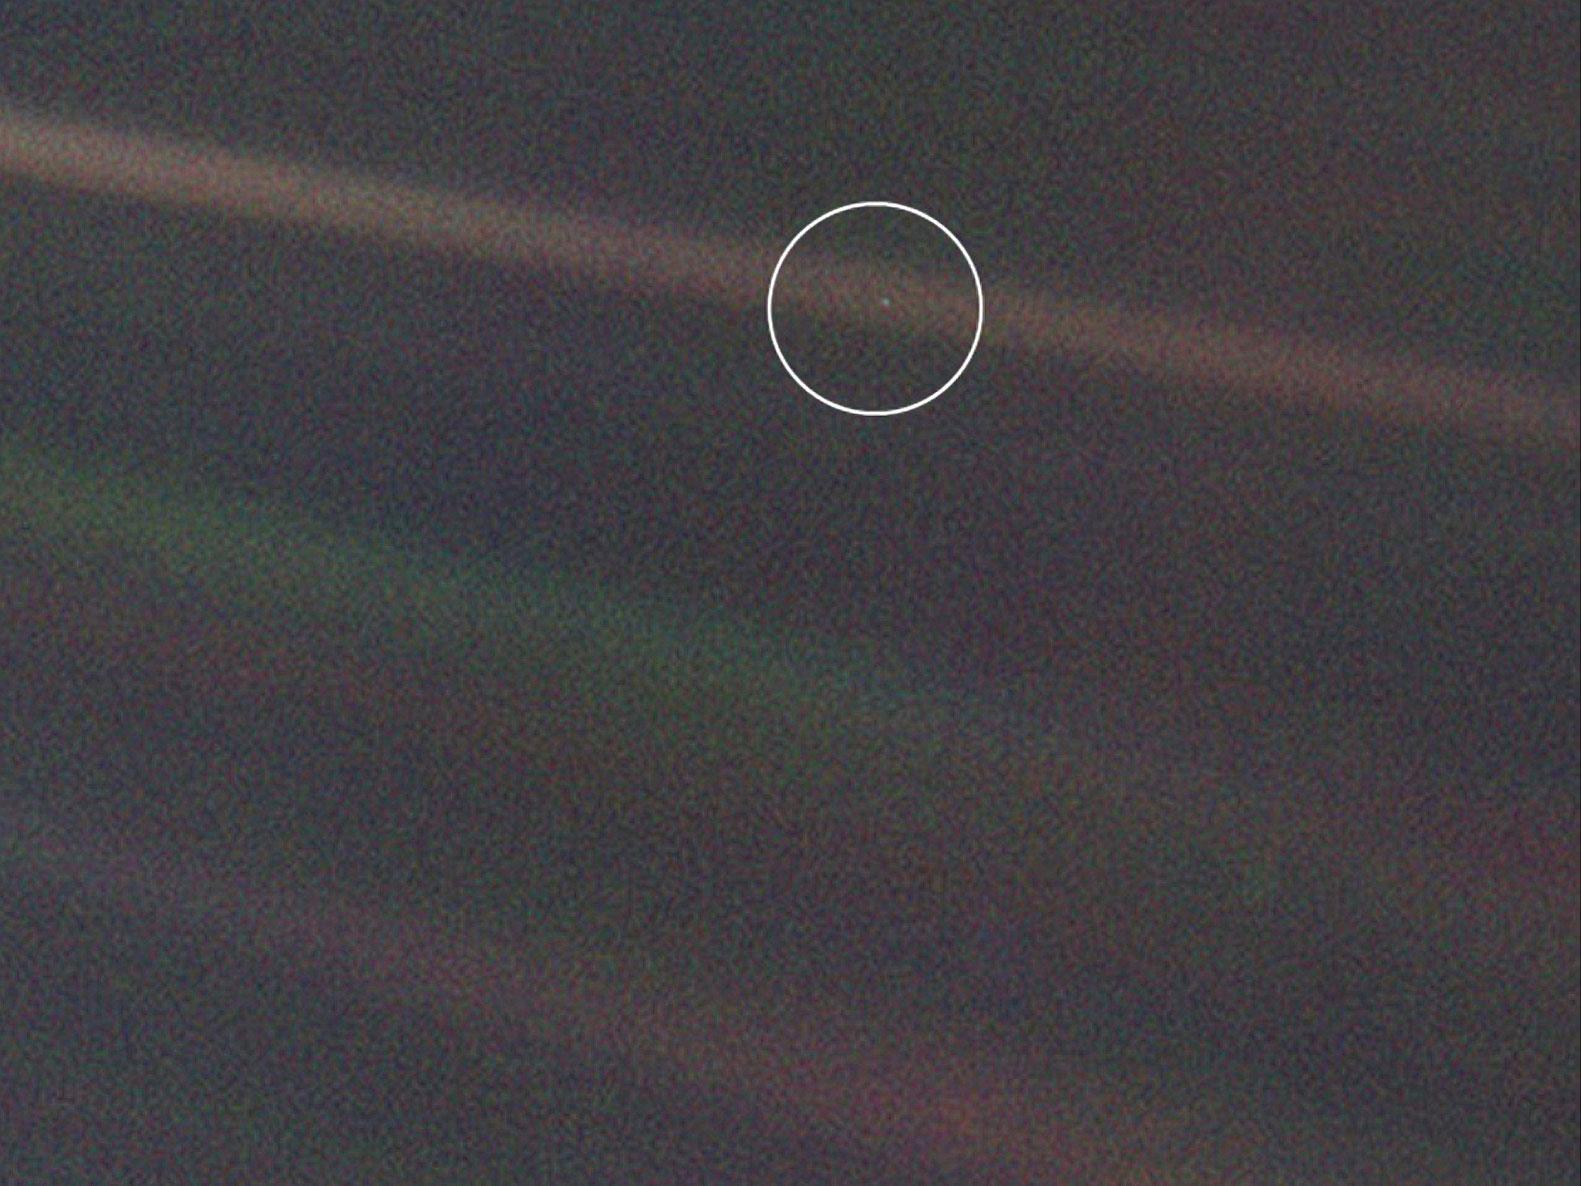
\includegraphics[width=\textwidth]{cover}

  \vspace*{\fill}

  \Huge{\textbf{\@title}}

  \vspace*{1cm}

  \Large\textit{\authors}

  \vspace*{\fill}

  \makeatother
\end{titlepage}

%\maketitle

%    Dedication.  If the dedication is longer than a line or two,
%    remove the centering instructions and the line break.
\cleardoublepage
\thispagestyle{empty}\mbox{}
\clearpage
\thispagestyle{empty}
\vspace*{13.5pc}
\begin{center}
  These Level Three notes are dedicated to\\[2pt] those who inspired me to learn physics.
\end{center}
\vspace*{\fill}
\begin{center}
  The cover photo shows the earth, as seen from the Voyager I spacecraft in 1990. The photograph was taken from a
  distance of around \SI{6e9}{\kilo\metre} away (forty times the distance from the earth to the sun).
\end{center}
\vspace*{6.75pc}
\cleardoublepage

%   Change page number to 6 if a dedication is present.
\setcounter{page}{6}

\tableofcontents

\chapter*{Introduction}
\begin{center}
  \emph{Or, a philosophical rant on the purpose of Level Three physics.}
\end{center}
Level 3 Physics is an extension of the material taught (learned?) at Level 2, and as such it
is a good idea to revise that material --- we will spend little to no time here doing so. Like
my Level 2 notes, this document does not include many exercises and is designed to be read in
conjunction with either past exams or some kind of problem book.

We cover the four content-heavy standards (mechanical systems, wave systems, electrical systems,
and modern physics) in some detail. I do expect a degree of mathematical maturity at least at the
level of M/E in the two level 2 mathematics external standards (algebra and calculus), and a concurrent
study of level 3 calculus is highly recommended. Exercises marked with a single asterisk* require
the usage of calculus. Some of the mathematical results required are summarised in the mathematical
review chapter beginning on page \pageref{chap:review}.

Any person wishing to go on to study physics at university should be aiming for M/E in all four of
the standards which we talk about, as well as the three external level 3 mathematics standards (the two
calculus standards and algebra). It is certainly possible to continue with an achieved this year, but
it will be very difficult and require a lot more work.

Some of the content that we cover this year is technically and conceptually difficult; I would urge
readers to not give up as it is often not until the chapter or section is completed that the `big
picture' can be seen. Unfortunately, physics is not only the purest and the most rewarding science;
it also has some of the hardest problems outside of mathematics. If you give up, you will have not
achieved anything more than wasting a year of your time.

\marginsymbol Throughout your study, you should try to understand not only the detail of the derivations and the results,
but the point of the whole exercise. You should always ask yourself the simple question, `what is the point
of this?'. In the electromagnetism standard, for example, it is up to you to build your own conceptual
understanding of the results:- there is a lot more theory than last year, and if you cannot provide your
own motivation (perhaps the beauty of the theory) then you will struggle.

On the other hand, despite the terse and unforgiving nature of the notes, I hope you enjoy forging your
own path into a slightly better understanding of the natural world!

\clearpage
\section*{What material is examinable?}
I have included a lot of extension and interest material (especially in the modern physics topic); however, I have made
the conscious decision to not explicitly mark it (except in a couple of cases). This is because context is very important
for understanding of physics, even at level three.

\emph{When I write practice scholarship exams, I pull freely from the interest material as well as the formal NCEA material. I
      am not so mean as to examine on the details, but I may (read: will) ask questions that use the extension material as a context.}

In other words, the answer to the title question is `your entire life until this point'. What will be on the test, then? Ink.

\section*{Special exercises}
I have decided to put in some field trips (\dsrailways) around Greater Wellington, and some experiments (\Radioactivity)
that you can perform on your own. Obviously these are not required, and your school may do some of them with you anyway.
However, they should be interesting!

\section*{Note on the chapter order}
I have decided to cover waves after mechanics and modern physics after electromagnetism since it is, to my mind,
a more natural progression than the actual order of the standards. Many schools choose to teach electromagnetism
last (for some reason), and so I have endeavored to avoid using too many ideas from electrodynamics in the modern
physics section. Beyond that, each part begins with a short introduction to the topic that it covers.

\vspace*{\fill}

\begin{aquote}{Norbert Wiener}
  The price of metaphor is eternal vigilance.
\end{aquote}

\chapter*{Mathematical Review}\label{chap:review}
\begin{aquote}{Silvanus P. Thompson}
  Considering how many fools can calculate, it is surprising that it should be thought either a difficult
  or a tedious task for any other fool to learn how to master the same tricks.
\end{aquote}

\emph{This chapter briefly reviews the mathematics that will be applied herein. It should not be used to learn
the skills, but merely to make sure that you are fluent in the basic computations and calculations required.}

\section*{Trigonometry}
The fundamental concept in trigonometry is the definition of the two basic trig functions (sine and cosine) based
on the unit circle. From this, we have the following:
\begin{multicols}{2}
  \noindent\begin{align*}
    \sin \theta &= \frac{\text{opposite}}{\text{hypotenuse}}\\
    \cos \theta &= \frac{\text{adjacent}}{\text{hypotenuse}}\\
    \tan \theta &= \frac{\sin \theta}{\cos \theta}
  \end{align*}
  \begin{align*}
    \csc \theta &= \frac{1}{\sin \theta}\\
    \sec \theta &= \frac{1}{\cos \theta}\\
    \cot \theta &= \frac{1}{\tan \theta}
  \end{align*}
\end{multicols}

\section*{Algebra}
If $ ax^2 + bx + c = 0 $ is a quadratic equation ($ a \neq 0 $), then
\begin{displaymath}
  x = \frac{-b \pm \sqrt{b^2 - 4ac}}{2a}.
\end{displaymath}

\section*{Calculus}
Let $ x $ be a value which changes over time. Then $ \frac{\Delta x}{\Delta t} $ is the average rate of change
of the quantity over that time period; if we let $ \Delta t \to 0 $, then we obtain the instantaneous rate of change
of $ x $, the \textbf{derivative of $ x $ with respect to $ t $}, denoted by $ \od{x}{t} $. The derivative of a function
$ f $ at a point $ x $ can also be denoted by $ f'(x) $.

Given the derivative $ f'(x) $, the \textbf{antiderivative} or \textbf{indefinite integral} of $ f' $ is
\begin{displaymath}
  \rint f'(x) \dif{x} = f(x) + C,
\end{displaymath}
where $ C $ is an arbitrary constant.

The area under the graph of a function $ f $ between the bounds $ x = a $ and $ x = b $ is the \textbf{definite integral},
and is denoted by
\begin{displaymath}
  \rint^b_a f'(x) \dif{x}.
\end{displaymath}

The \textbf{fundamental theorem of calculus} states that
\begin{displaymath}
  \rint^b_a f'(x) \dif{x} = f(b) - f(a).
\end{displaymath}

\section*{Tables of Derivatives}

\begin{center}
  \def\arraystretch{1.5}
  \begin{tabular}{|c|c|}\hline
    \textbf{Function} & \textbf{Derivative}\\\hline
    $ x^n $ & $ nx^{n - 1} $\\\hline
    $ e^x $ & $ e^x $\\\hline
    $ \ln \abs{x} $ & $ \frac{1}{x} $\\\hline
    $ \sin x $ & $ \cos x $\\\hline
    $ \cos x $ & $ -\sin x $\\\hline
    $ \tan x $ & $ \sec^2 x $\\\hline
    $ \csc x $ & $ -\csc x \cot x $\\\hline
    $ \sec x $ & $ \sec x \tan x $\\\hline
    $ \cot x $ & $ -\csc^2 x $\\\hline
  \end{tabular}
  \begin{tabular}{|c|c|c|c|}\hline
    \textbf{Function} & \textbf{Derivative} &
    \textbf{Function} & \textbf{Derivative}\\\hline
    $ \sin^{-1} x $ & $ \frac{1}{\sqrt{1 - x^2}} $ &
    $ \csc^{-1} x $ & $ -\frac{1}{x\sqrt{x^2 - 1}} $ \\\hline
    $ \cos^{-1} x $ & $ -\frac{1}{\sqrt{1 - x^2}} $ &
    $ \sec^{-1} x $ & $ \frac{1}{x\sqrt{x^2 - 1}} $\\\hline
    $ \tan^{-1} x $ & $ \frac{1}{1+x^2} $ &
    $ \cot^{-1} x $ & $ -\frac{1}{x^2 + 1}$\\\hline
  \end{tabular}
\end{center}

\begin{figure}
  \centering
  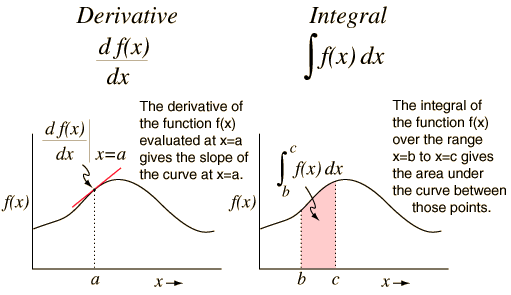
\includegraphics[width=\textwidth]{derint}
  \caption{The derivative and the integral.}\label{fig:lewin}
\end{figure}


%%%%%%%%%%%%%%%%%%%%
%%%%%%%%%%%%%%%%%%%%
%%%%%%%%%%%%%%%%%%%%
%%%%%%%%%%%%%%%%%%%%
%%%%%%%%%%%%%%%%%%%%
%%%%%%%%%%%%%%%%%%%%
%%%%%%%%%%%%%%%%%%%%
%%%%%%%%%%%%%%%%%%%%
%%%%%%%%%%%%%%%%%%%%
%%%%%%%%%%%%%%%%%%%%
%%%%%%%%%%%%%%%%%%%%
%%%%%%%%%%%%%%%%%%%%
%%%%%%%%%%%%%%%%%%%%
%%%%%%%%%%%%%%%%%%%%
%%%%%%%%%%%%%%%%%%%%
%%%%%%%%%%%%%%%%%%%%
%%%%%%%%%%%%%%%%%%%%
%%%%%%%%%%%%%%%%%%%%
%%%%%%%%%%%%%%%%%%%%


\swatchcolor{Emerald}
\partcover{mechcover}
\partintro{
  We begin our discussion of mechanics with a little revision from last year's study of linear mechanics, extending it
  to slightly more complex situations in 2D. We then introduce two new models:
  \begin{itemize}
    \item Angular motion (things moving in circles), and
    \item Simple harmonic motion (things moving backwards and forwards).
  \end{itemize}

  The punchline turns out to be that both of these models are, in fact, equivalent.
}
\part{Mechanical Systems}


\chapter{Linear Mechanics}
\begin{aquote}{Sir Isaac Newton}
  To explain all nature is too difficult a task for any one man or even for any one age. 'Tis much better to do a
  little with certainty, \& leave the rest for others that come after you, than to explain all things by conjecture
  without making sure of any thing.
\end{aquote}
\section{Force, momentum, energy, and work}
\emph{This section uses calculus to derive energy and work from Newton's law of force. If you were comfortable with the
calculations with energy and work done last year and are uncomforable with calculus, you can get away without reading this
section closely.}

The fundamental concepts of classical mechanics are those of force and momentum. Essentially, a force $ F $ is something
which can produce a change in motion; and momentum $ p = mv $ is the `quantity of motion' of a body. We can write down Newton's
second law $ F = ma $ in terms of force and momentum:
\begin{equation}
  F = \od{p}{t}
\end{equation}
This equation reads most naturally as `the change of momentum with respect to time is called force', but a better way to think
about this relationship is that `a force produces a corresponding change in momentum'.

Now, suppose that a force acts on an object while the object moves a particular distance at a constant speed (perhaps we are
providing a force against gravity). A natural question to ask is `how much force did we put into our system in order to move
that object', or `how much work did it take'? We wish to sum together all of the instantaneous forces which we apply over the
distance from $ x_0 $ to $ x_1 $; this is just an integral:
\begin{displaymath}
  \rint_{x_0}^{x_1} F \dif{x} = \rint_{x_0}^{x_1} \od{p}{t} \dif{x}
\end{displaymath}
Now we can evaluate the right-hand side via the chain rule and the definition of momentum:
\begin{displaymath}
  \rint_{x_0}^{x_1} \od{p}{t} \dif{x} = \rint_{x_0}^{x_1} m \od{v}{t} \dif{x} = \rint_{v_0}^{v_1} m \od{x}{t} \dif{v}
    = \rint_{v_0}^{v_1} mv \dif{v} = \frac{1}{2}mv_1^2 - \frac{1}{2}mv_0^2.
\end{displaymath}
and overall, we have the following identity:
\begin{displaymath}
  \rint_a^b F \dif{x} = \frac{1}{2}mv_0^2 - \frac{1}{2}mv_1^2
\end{displaymath}
We define the quantity on the left (the `total amount of force' we put in) to be \textbf{work} ($ W $), and the quantity on
the right to be the change in \textbf{kinetic energy} ($ \Delta E_k $) when the object is accelerated from $ v_0 $ to $ v_1 $.

If the force is constant, then $ W = F\Delta x $ and
\begin{equation}
  W = F \Delta x = \Delta E_k.
\end{equation}

Now consider Hooke's law, where the force is directly proportional to displacement. We have $ F = kx $ for some constant $ k $; then:
\begin{equation}\label{eqn:elenergy}
  W = \rint_{x_0}^{x_1} kx \dif{x} = \frac{1}{2}kx_1^2 - \frac{1}{2}kx_0^2 = \Delta U_\ell.
\end{equation}
Again, the quantity on the right is the change in `energy': this time, \textbf{elastic potential energy}.

\emph{Work and changes in energy are simply the `amount of force' that we need to put into a system to get something done.}

Some common types of energy include:
\begin{itemize}
  \item The energies associated with \textbf{position} (called \textbf{potential energies}):
    \begin{itemize}
      \item Gravitational potential energy.
      \item Electric potential energy.
      \item Chemical potential energy.
      \item Elastic potential energy.
    \end{itemize}
  \item The energies associated with \textbf{motion} (called \textbf{mechanical energies}):
    \begin{itemize}
      \item Linear kinetic energy.
      \item Rotational kinetic energy.
      \item Thermal energy.
    \end{itemize}
\end{itemize}
In each case, we can derive formulae for the energies by integrating the respective forces.

The units of energy and work are joules (J). We use the symbol $ E $ for mechanical energies, and $ U $ for potential energies.

Energy is always conserved in any system: we can only interact with a system through forces, and those forces are just transfers of
energy, so at no point is energy lost or gained. Energy can only be transformed from one form to another. \emph{Note that it is
not necessarily the case that \emph{mechanical} energy is conserved.}

\begin{exercise}
  For the following scenarios, fully describe the energy changes that occur.
  \begin{enumerate}
    \item Amanda is bungee-jumping in Rotorua. Her head just touches the water at the bottom of her jump.
    \item Bob eats an apple and walks to the compost bin to throw out the core.
    \item Carol presses a button to electrically detonate high explosives in the bottom of a mine.
    \item David stands perfectly still at the North Pole.
  \end{enumerate}
\end{exercise}

\begin{exercise}
  Energy is only conserved in \textit{closed systems}. Define the notion of closed system.
\end{exercise}

\begin{exercise}
  Two cars collide and come to a complete stop. Where did their energy go?
\end{exercise}

\begin{figure}
  \centering
  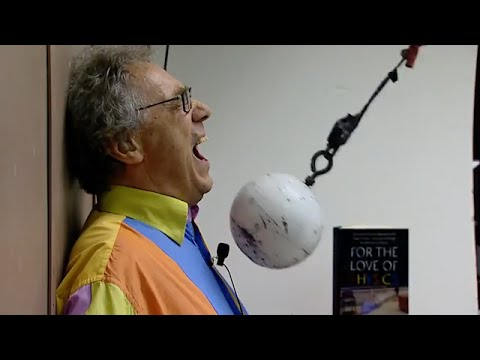
\includegraphics[width=0.6\textwidth]{lewin}
  \caption{Walter Lewin.}\label{fig:lewin}
\end{figure}

\begin{exercise}
  A famous physics lecturer (\cref{fig:lewin}) gives a demonstration that involves standing at one side of the lecture theatre
  and releasing a \SI{50}{\kilo\gram} steel ball that can swing freely like a pendulum. Explain why, when the
  ball swings back, it does not crush him.
\end{exercise}

You can even watch Walter Lewin performing this experiment in a lecture:
\goandwatch{https://www.youtube.com/watch?v=xXXF2C-vrQE}

\section{Centre of Mass}
\begin{figure}
  \centering
  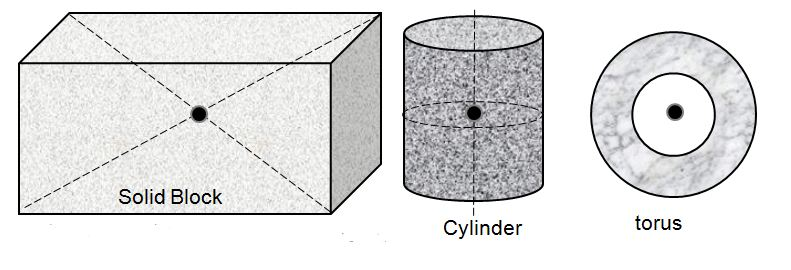
\includegraphics[width=0.6\textwidth]{centreofmass2}
  \caption{The centre of mass of several 3D objects.}\label{fig:centreofmass2}
\end{figure}
It is obvious `where' a force acts on a point-particle like an electron. However, if a force acts on a larger object --- like a car --- it is
not obvious how a force acts. The \textbf{centre of mass} is the point in a larger object through which any force appears to act, and it is
the `average centre' of the object taking into account the object's distribution of mass.

We more precisely define the centre of mass as the location at which the weighted position vectors of each point (vectors whose direction is
from the location towards the point, and whose length is multiplied by the mass of that point) add up to zero.

Note that, as in the torus depicted in \cref{fig:centreofmass2}, it is possible for the centre of mass to lie outside the object!

\begin{figure}
  \centering
  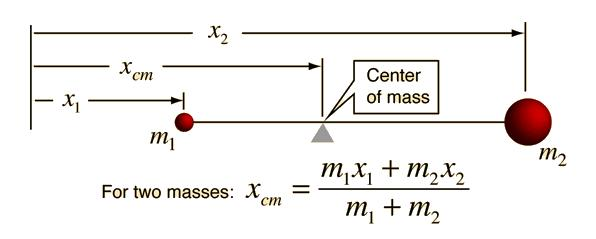
\includegraphics[width=0.7\textwidth]{centreofmass}
  \caption{The centre of mass of two particles.}\label{fig:centreofmass}
\end{figure}

If we have two particles (\cref{fig:centreofmass}), of mass $ m_1 $ and $ m_2 $, we wish to find at which point between them their centre
of mass lies. Let's choose a coordinate system so that both particles are on the $ x$-axis, with coordinates $ x_1 $ and $ x_2 $. Suppose
that the centre of mass is at $ x_{\cm} $; then the weighted position vectors are $ m_1 (x_1 - x_\cm) $ and $ m_2 (x_2 - x_\cm) $ ---
so $ m_1 (x_1 - x_\cm) + m_2 (x_2 - x_\cm) = 0 $, and (solving for $ x_\cm $) we have:
\begin{equation}
  x_\cm = \frac{m_1 x_1 + m_2 x_2}{m_1 + m_2}.
\end{equation}

In general, for $ n $ masses, we have:
\begin{equation}
  x_\cm = \frac{\sum_{i = 0}^n m_i x_i}{\sum_{i = 0}^n m_i}.
\end{equation}

\begin{exercise}
  Find the centre of mass of a three-particle system, where the particles are at $ (0, 0) $, $ (3, 0) $, and $ (-5, 0) $ and have respective masses
  of 1, 2, and 3 kilograms.
\end{exercise}

The centre of mass of a 2D system of discrete particles is simply at the intersection of the two 1D centres of mass:
\begin{equation}
  (x,y)_\cm = \left(\frac{\sum_{i = 0}^n m_i x_i}{\sum_{i = 0}^n m_i}, \frac{\sum_{i = 0}^n m_i y_i}{\sum_{i = 0}^n m_i} \right).
\end{equation}

\begin{exercise}
  Consider a three-particle system, where the particles are at $ (-2, 1) $, $ (4, 1) $, and $ (1, -1) $ and have respective masses
  of 2, 2, and 3 kilograms. Plot the particles and the centre-of-mass.
\end{exercise}

\begin{figure}
  \centering
  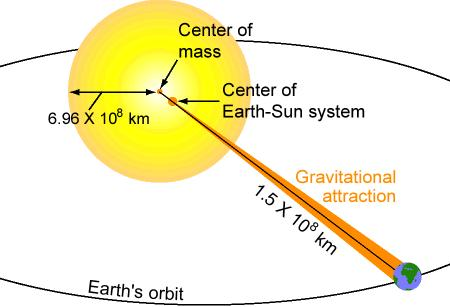
\includegraphics[width=0.5\textwidth]{sunsystem}
  \caption{The centre of mass of the sun/earth orbital system.}\label{fig:sunsystem}
\end{figure}

\begin{exercise}
  The moon, the earth, and the sun are orbiting each other around their common centre of mass. Using the following data, calculate
  the average distance from the earth's centre that their centre of mass lies.
  \begin{center}
    \def\arraystretch{1.5}
    \begin{tabular}{ll}\hline
      Mass of Earth & \SI{5.972e24}{\kilo\gram}\\\hline
      Mass of Moon & \SI{7.348e22}{\kilo\gram}\\\hline
      Mass of Sun & \SI{1.989e30}{\kilo\gram}\\\hline
      Average distance between Sun and Earth & \SI{149.6e8}{\kilo\metre}\\\hline
      Average distance between Moon and Earth & \SI{384500}{\kilo\metre}\\\hline
    \end{tabular}
  \end{center}
  [\emph{Hint: the moon is much closer to the earth than to the sun.}]
\end{exercise}

\begin{experiment}
  Cut out some irregular shapes from a sheet of cardboard, some with holes in them; find the centre of mass (balance point) of each one. Can
  you come up with a general experimental method that allows you to find the centre of mass of any 2D
  object?\footnote{~For the `standard' way of doing this, search for `plumb line centre of mass' on the
  internet --- but try to come up with your own method first!}
\end{experiment}

\section{Conservation of Momentum}
Momentum is a quantity that is always preserved --- in a closed system, $ p_i = p_f $. We need to be careful when working in two dimensions,
however, since momentum is a \emph{vector quantity}; it is not just the \emph{amount} of momentum that is conserved, but the \emph{direction}
as well.

\begin{exercise}
  A metal box of mass $ M $ is free to slide on a frictionless, horizontal surface. A metal ball of mass $ M/4 $ is fired with
  velocity $ V $ at the block, and bounces straight backwards off the block with one third of its original speed.
  \begin{enumerate}
    \item What is the final speed $ V_f $ of the block after the impact in terms of $ M $ and $ V $?
    \item Is kinetic energy conserved in this collision? If not, how much energy is lost?
  \end{enumerate}
\end{exercise}

\begin{exercise}
  A system of two particles linked with a rigid rod of negligible mass, instantaneously located at $ (-3,0) $ and $ (2, 0) $ and
  with respective masses of \SI{500}{\gram} and \SI{750}{\gram}, is moving at a constant speed of \SI{5}{\metre\per\second}.
  \begin{enumerate}
    \item How far from the \SI{500}{\gram} particle is the centre of mass of the system?
    \item What is the momentum of the system?
  \end{enumerate}
\end{exercise}

Since force is the time derivative of momentum, we can write
\begin{equation}
  \Delta p = \rint F \dif{t}.
\end{equation}

This change in momentum is called the \textbf{impulse}.

\begin{exercise}
  A rubber ball (of mass $ m $) and a sticky ball (of mass $ 2m $) are thrown at a wall with equal speeds $ v $. The
  rubber ball bounces off, while the sticky ball sticks to the wall. Which ball delivers a greater impulse to the wall?
\end{exercise}

\begin{exercise}
  A \SI{50}{\gram} ball moving at a speed $ v_0 $ hits and sticks to a \SI{1.0}{\kilo\gram} brick sitting at rest on
  a frictionless surface. Compute the speed of the brick-ball mass after the collision, and decide whether the collision
  was \textbf{elastic}.\footnote{~An elastic collision is one in which mechanical energy is conserved.}
\end{exercise}

\begin{exercise*}
  Suppose a particle has momentum \SI{30}{\kilo\gram \metre\per\second} at time $ t = 0 $, and is brought to a stop in
  a force field changing over time and described by $ F(t) = 4t - 3t^2 $. At what time $ t $ does the particle stop?
\end{exercise*}

\section{Circular Motion}
\begin{figure}
  \centering
  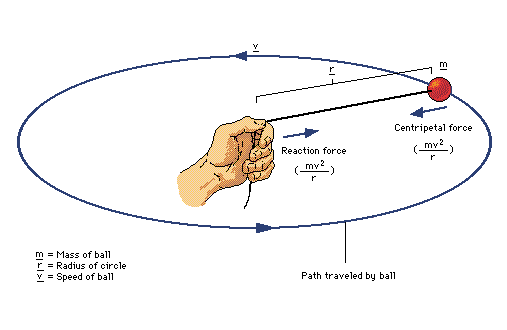
\includegraphics[width=0.9\textwidth]{centripetal}
  \caption{A force which causes circular motion is called a centripetal force. \capcite{https://i.pinimg.com/originals/74/d2/28/74d228e85a6a3f4fb700bcafa677539d.gif}\label{fig:centripetal}}
\end{figure}
If a particle is moving in a circle at a constant speed, then its velocity is changing and so it is accelerating. By
Newton's second law, there must be an unbalanced force acting on the particle (and it must be pointing perpendicular to
the instantaneous motion of the particle, towards the centre of the movement). This force is known as a \textbf{centripetal force}.

\begin{exercise}
  Explain the phenomenon of `centrifugal force' --- the apparent force that pushes a person to the outside of the
  turning circle when a car turns.
\end{exercise}

I put this video in the Level 2 notes, but it is well worth another watch.
\goandwatch{https://www.youtube.com/watch?v=zHpAifN_2Sw}

Suppose the particle is moving at a constant velocity $ v $ around a circle of radius $ r $. Then the \textbf{centripetal
acceleration} is given by
\begin{equation}
  a_c = \frac{v^2}{r},
\end{equation}
and the centripetal force acting (if the particle has mass $ m $) is:
\begin{equation}
  F_c = \frac{mv^2}{r},
\end{equation}

We can derive the centripetal acceleration in an intuitive way as follows. Consider an object of mass $ m $ moving at a constant speed $ v $ around a
circle of radius $ r $. The position of the object can be represented by a rotating vector (a \textbf{phasor}); the total distance covered by the end
of the vector after one cycle is $ 2 \pi r $. This is the total amount that the position of the particle changes in one cycle.

We can also represent the velocity of this object in the same way: as the particle moves around the circle, the velocity
vector of the particle makes a complete circle as well. Hence the total amount that the velocity of the particle changes
in one period is $ 2\pi v $.

It follows then that the constant acceleration of the particle is, as we claimed, $ a = \frac{\Delta v}{\Delta t} = \frac{2\pi v}{2\pi r / v} = \frac{v^2}{r} $.

\begin{exercise}
  A red ball of mass \SI{4}{\kilo\gram} is moving at a constant speed in a circle of radius \SI{4}{\metre}.
  \begin{enumerate}
    \item The frequency of the ball's motion is \SI{0.5}{\hertz}. What is the speed of the ball around the circle?
    \item Give the centripetal force acting on the ball to keep it in the circle.
  \end{enumerate}
\end{exercise}

\begin{exercise}
  A car of mass \SI{2000}{\kilo\gram} is moving around an unbanked bend of radius \SI{30}{\metre}. The maximum friction
  force between the wheels and road is \SI{320}{\newton}. What is the highest speed that the car can drive around the
  curve without skidding? What if the bend is banked at \SI{20}{\degree}?
\end{exercise}

In the next chapter, we will extend our understanding of rotational motion from constant rotational speed
to changing rotational speed. Before that, we will discuss Newton's law of gravity.

\section{Gravity}
\begin{figure}
  \centering
  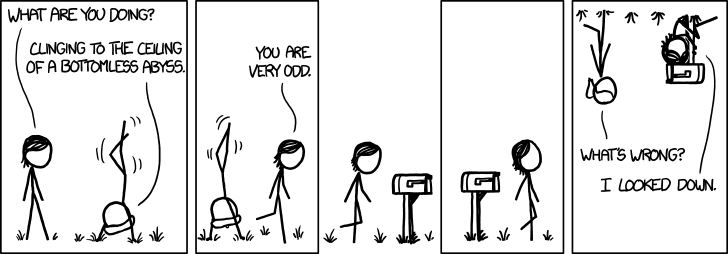
\includegraphics[width=0.8\textwidth]{sky}
  \caption{I dropped a bird and I didn't hear it hit bottom. \capcite{https://xkcd.com/1115/}\label{fig:sky}}
\end{figure}
\begin{figure}
  \centering
  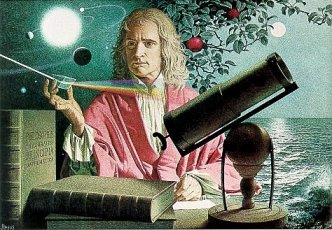
\includegraphics[width=0.7\textwidth]{newton}
  \caption{Sir Isaac Newton. \capcite{http://teachertech.rice.edu/Participants/louviere/Newton/newton5.jpg}\label{fig:newton}}
\end{figure}
The classical law of gravity was first described by Sir Isaac Newton (\cref{fig:newton}) in 1986. It states that the force of
gravity $ F_G $ between two particles is directly proportional to the masses $ m $ and $ M $ of the particles, and inversely
proportional to the square of the distance $ r $ between them:
\begin{equation}
  F_G = G\frac{mM}{r^2}.
\end{equation}
The constant $ G $ is \SI{6.674e-11}{\newton\metre\squared\per\kilo\gram\squared}.

\begin{exercise}
  Use dimensional analysis to confirm the units of $ G $.
\end{exercise}

We can use this law to derive the value of $ g $, the acceleration due to gravity on earth. Let $ m $ be the mass of the object, and $ M $ the
mass of the earth. We have $ mg = G\frac{mM}{r^2} $, so $ g = \frac{GM}{r^2} = \frac{\num{6.674e-11} \times \num{5.972e24}}{(\num{6371e3})^2} $
(since the distance between the centre of the earth and the centre of mass of the object is approximately the radius of the earth) and
so $ g \approx \SI{9.8195}{\metre\per\second\squared} $.\footnote{~A more accurate calculation or measurement gives the value
as \SI{9.807}{\metre\per\second\squared}, so even with our imprecise values for $ M $ and $ r $ we are not too far off.}

\begin{figure}
  \centering
  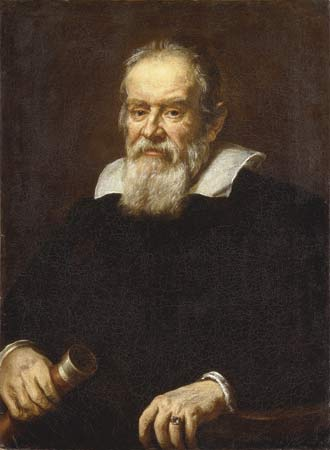
\includegraphics[width=0.4\textwidth]{galileo}
  \caption{Galileo Galilei. \capcite{https://media1.britannica.com/eb-media/58/95758-004-BD98B43B.jpg}\label{fig:galileo}}
\end{figure}

The interesting thing about this calculation is that it shows that all objects fall at the same rate due to gravity! While two objects with
different masses will feel different forces, their accelerations from zero will be the same and so will reach the ground at the same time. An
experiment to demonstrate this was first performed by Galileo Galilei (\cref{fig:galileo}) in the late 1500s, when he allegedly dropped two
spheres of different masses off the Leaning Tower of Pisa.

Apollo 15 astronaut David Scott repeated a similar experiment on the moon with a feather and a hammer.

\goandwatch{https://www.youtube.com/watch?v=5C5_dOEyAfk}

\begin{figure}
  \centering
  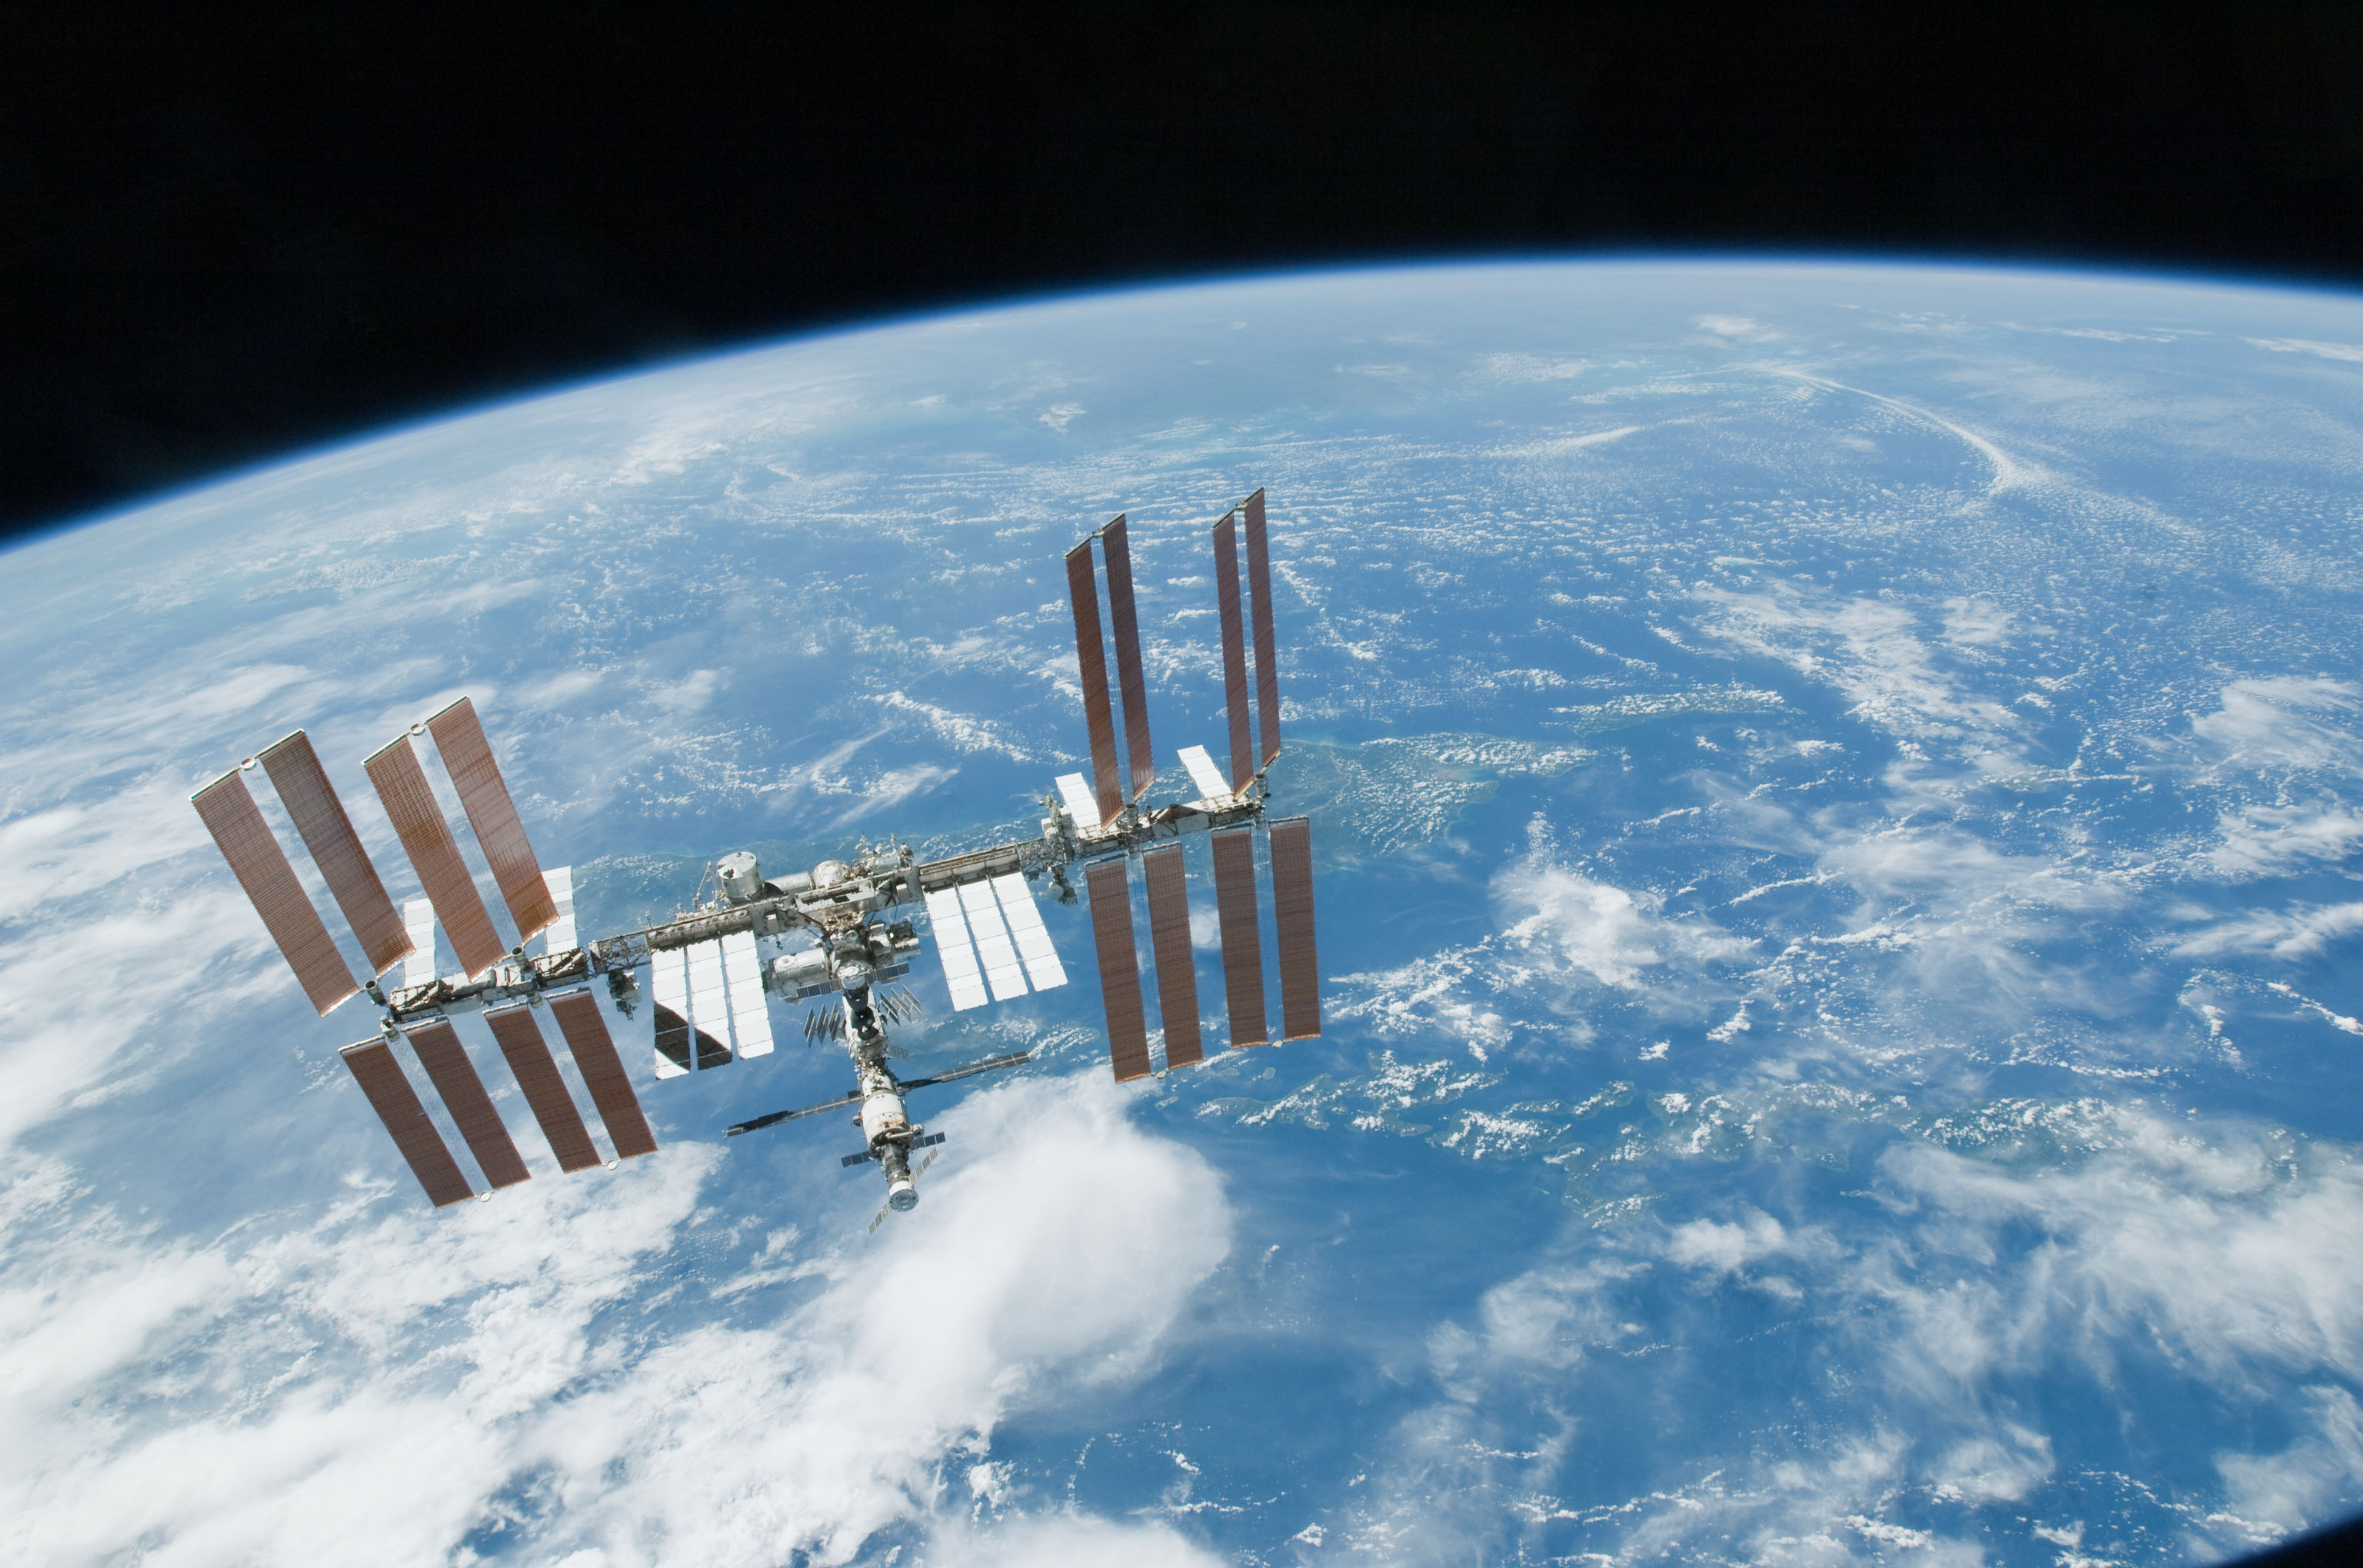
\includegraphics[width=0.6\textwidth]{iss}
  \caption{The International Space Station.\label{fig:iss}}
\end{figure}
\begin{exercise}
  Gravitational force calculations are important for calculations of escape velocities; hence, this question is literally rocket science.
  \begin{enumerate}
    \item The International Space Station (\cref{fig:iss}) orbits at a height of around \SI{404}{\kilo\metre} above the earth's surface. How
          fast must it be travelling?  [\emph{Hint: draw a force diagram.}]
    \item In general, show that the speed of a satellite in a circular orbit around some mass $ M $ at height $ r $ is exactly $ v = \sqrt{GM/r} $.
  \end{enumerate}
\end{exercise}

\begin{exercise}
  Mars has a mass of 0.107 Earths, and an average radius of \SI{3389.5}{\kilo\metre}. What is the acceleration due to Mars' gravity
  at its surface?
\end{exercise}

\begin{exercise}
  A satellite orbits the moon at a height of \SI{55}{\kilo\metre} above the surface. The radius of the moon is \SI{1.7e6}{\metre}, and the
  mass of the moon is \SI{7.3e22}{\kilo\gram}. What is the radius of the orbit of the satellite?
\end{exercise}

\begin{experiment}
  Devise and carry out an experiment to determine the value of the gravitational constant, $ G $.
\end{experiment}

\begin{exercise}
  This exercise is an application of the physics of this chapter to a real-life problem.

  \begin{enumerate}
    \item Suppose that we take an empty universe and add into it two masses, $ M $ and $ m $, at a distance $ r $ apart. What is the total
            potential energy (due to gravity) in this universe? [Hint: calculate the total work required to pull them apart.]
    \item Hence calculate the amount of kinetic energy gained by a meteor as it moves from space (\SI{100}{\kilo\metre} above the surface of Earth)
            to the ground.
    \item The original speed of a meteor as it enters the atmosphere ranges from \num{11} to \SI{72}{\kilo\metre\per\second}. Calculate the theoretical
            total kinetic energy of the meteor as it hits the ground.
    \item Let us arrange matters such that our meteor hits a giant block of solid diamond. The vapourisation energy of carbon
            is \SI{715}{\kilo\joule\per\mole}, and the molar volume of diamond is \SI{3.42}{\centi\metre\cubed\per\mole}. What
            volume of carbon is vapourised, and what is the radius of the crater (remember that the meteor explodes on impact, so the
            crater will be a hemisphere not a sphere)?
    \item Suggest a possible use for such a crater.
  \end{enumerate}
\end{exercise}

You can use part (1) of the above exercise to calculate escape speeds using energy conservation.\footnote{~Knight, ch. 13}

\chapter{Rotational Mechanics}
\begin{aquote}{Archimedes}
  Do not disturb my circles!
\end{aquote}
\section{Angular Motion}
\begin{figure}
  \centering
  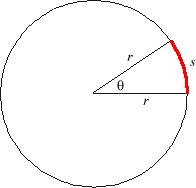
\includegraphics[width=0.3\textwidth]{radian}
  \caption{An angle in a circle cuts off a particular arc length.\label{fig:radians}}
\end{figure}
In this chapter, our goal is to extend our definitions of \textbf{position}, \textbf{speed}, and \textbf{acceleration} from a linear
setting to a rotational setting; in doing so, we will see that every concept of linear motion has an exact rotational counterpart.

The definition and use of \textbf{radians} as a unit of angle measure should be familiar to you; briefly, we define the
angle $ \theta $ to be the ratio between the arc length $ s $ and the radius $ r $ (\cref{fig:radians}).

\begin{exercise}
  Show that radians are unitless.
\end{exercise}

Now, consider a particle moving (perhaps at a non-constant speed) around a circle of fixed radius $ r $. At each time, we can measure
its angle $ \theta $ away from some zero-point on the circle; this is the \textbf{angular position} of the particle. We define the
\textbf{angular velocity} $ \omega $\footnote{~The Greek letter \textbf{omega}.} and the \textbf{angular acceleration} $ \alpha $
in an analagous way to those of their linear counterparts:
\begin{gather}
  \omega = \dod{\theta}{t}\\
  \alpha = \dod{\omega}{t} = \dod[2]{\theta}{t}
\end{gather}

\begin{figure}
  \centering
  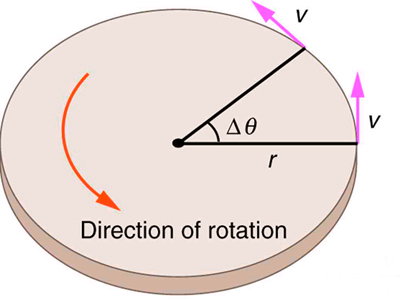
\includegraphics[width=0.7\textwidth]{angvelocity}
  \caption{The relationship between angular velocity of a rotating object, and the linear velocity of a point at its edge.\label{fig:angvelocity}}
\end{figure}

Suppose that the speed of the particle around the edge of the circle is $ v $ at some moment (\cref{fig:angvelocity}). Then we have $ \od{s}{t} = v $;
but since $ s = r\theta $, $ \od{s}{t} = r\od{\theta}{t} $ (by the chain rule) and:
\begin{equation}
  v = r\omega.
\end{equation}
Similarly, for the acceleration of the particle around the circle,
\begin{equation}
  a = r\alpha.
\end{equation}

\begin{exercise}
  Show that $ \SI{1}{\rpm} \equiv \SI{0.1047}{\radian\per\second} $.\footnote{~rpm: revolutions per minute.}
\end{exercise}

\begin{example}
  \SI{44}{\metre} of cable are pulled off a cable drum with a radius of \SI{0.2}{\metre}. It takes \SI{22}{\second} to unwind
  the cable at a steady speed.
  \begin{enumerate}
    \item Through what angular displacement does the drum turn?
    \item Through how many revolutions does the drum turn?
    \item What is the angular velocity of the drum?
    \item What is the linear speed of the cable being pulled from the drum?
  \end{enumerate}
\end{example}
\begin{solution}
  The circumference of the drum is $ 2\pi \times 0.2 = 1.2566 $. Hence the drum turns through $ 44/1.2566 = 35 $ revolutions,
  or $ 70\pi~\si{\radian} $. The angular velocity of the drum is therefore
  \begin{displaymath}
    \omega = \frac{\Delta \theta}{\Delta t} = \frac{70\pi}{22} = \SI{10}{\radian\per\second},
  \end{displaymath}
  and the linear speed of the wire is $ v = r\omega = 0.22 \times 10 = \SI{2.2}{\metre\per\second} $.
\end{solution}

The earth is rotating about an axis through the north and south poles. The surface of the earth has a linear velocity die to this
rotation; the equator, being the greatest distance from the centre (so having the largest possible radius of any part of the surface
of the planet), has the highest linear velocity (around \SI{1600}{\kilo\metre\per\hour}). Because of this, most major space launch
sites are located as close to the equator as possible so that the amount of `kick' from the earth's own rotation is greatest.

Now, suppose we want to find the relationship of the frequency of rotation to the angular velocity. There are $ 2\pi $ radians
in a circle, so $ \frac{1}{f} \omega = 2\pi $ (since $ 1/f $ is the time taken for one revolution), and we have
\begin{equation}
  \omega = 2\pi f.
\end{equation}

\begin{exercise}
  A helicopter blade is rotating at a speed of \SI{529.8}{\rpm}, and has a diameter of \SI{7.67}{\metre}. What is the angular
  velocity of the blade, and how fast is the tip of the blade moving?
\end{exercise}

\begin{figure}
  \centering
  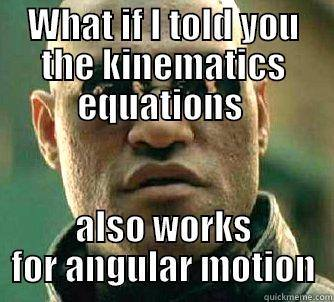
\includegraphics[width=0.7\textwidth]{kinematics}
  \caption{It's true.\label{fig:kinematics}}
\end{figure}

We have \textbf{rotational kinematic equations} for constant angular acceleration that are exactly analagous to those describing linear motion.
\begin{gather}
  \omega_f = \omega_i + \alpha t\\
  \theta = \frac{\omega_i + \omega_f}{2}\\
  \theta = \omega_i t + \frac{1}{2} \alpha t^2\\
  \omega_f^2 = \omega_i^2 + 2 \alpha \theta
\end{gather}

To derive these equations, we can use very simple Level 2 calculus (remembering that $ \alpha $ is constant). For example:
\begin{gather*}
  \alpha t = \rint_{t_i}^{t_f} \alpha \dif{t} = \rint_{t_i}^{t_f} \od{\omega}{t} \dif{t} = \omega_f - \omega_i \Rightarrow \omega_f = \omega_i + \alpha t\\
\end{gather*}

\begin{exercise*}
  Derive the other rotational kinematic equations.
\end{exercise*}

\begin{exercise}
  When switched off, an electric fan takes \SI{15}{\second} to come to a complete stop. During this time,
  30.5 revolutions are completed. Assuming that the angular deceleration was constant, what was its magnitude?
\end{exercise}

\begin{exercise}
  A car with \SI{80}{\centi\metre} diameter wheels starts from rest and accelerates uniformly to a velocity of \SI{20}{\metre\per\second}
  over \SI{9.0}{\second}. Find the angular acceleration and final angular velocity of one of its wheels.
\end{exercise}

\section{Torques}
\begin{figure}
  \centering
  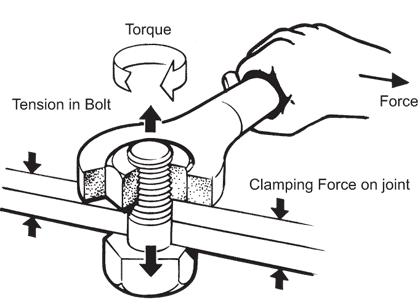
\includegraphics[width=0.7\textwidth]{torque}
  \caption{A force on a wrench producing a torque around an axis.\label{fig:torque}}
\end{figure}
The rotational counterpart of force is called \textbf{torque} (symbol $ \tau $). The size of the torque depends
on the size $ F $ of the force inducing the turning effect, and on the perpendicular distance $ r $ from the force
to the axis of rotation. In \cref{fig:torque} above, the torque produced is due to a force on a wrench. If the
force was moved further away but did not increase in magnitude, the torque induced would increase; we formally
define the torque by
\begin{equation}
  \tau = Fr.
\end{equation}

\textbf{Being able to take torque moments around an axis is an important skill that you should revise from last year.}

\begin{exercise}
  A force $ F $ is applied perpendicular to a wrench at a distance $ x $ from the head to produce a torque $ \tau $.
  If the distance from the head to the force is quadrupled, by what factor must the force be multiplied to produce the
  same torque?
\end{exercise}

\begin{exercise}
  The bicep muscle of a weight lifter exerts a vertical force of \SI{50}{\newton} on his lower arm, \SI{5.0}{\centi\metre} away from
  the elbow joint. If the muscle is parallel to the upper arm, and the arm is bent at a right angle, what torque does the bicep place
  on the lower arm about the elbow? What is the mass of the barbell the weight lifter can support in his hand \SI{25}{\centi\metre}
  away from the elbow with this torque?
\end{exercise}

\begin{trip}
  Visit the Zephyrometer at the corner of Cobham Drive and Evans Bay Parade. By estimating the mass of the counterweight, the length of
  the arm, and the angle of deflection by the wind, calculate the force exerted by the average Wellington southerly breeze.
\end{trip}

\section{Rotational Inertia and Momentum}
The quantity of \textbf{rotational inertia} (or \textbf{moment of inertia}) plays the same role for angular motion that mass does for
linear motion --- it is a measure of the resistance of the body to angular acceleration. We define it to be
\begin{equation}
  I = \sum mr^2,
\end{equation}
where we sum over each point mass in the system ($ r $ being the distance of the point from the axis of rotation). If
a mass is continuous, then the sum becomes an integral.

\begin{exercise}
  Find the units of $ I $.
\end{exercise}

\begin{figure}
  \centering
  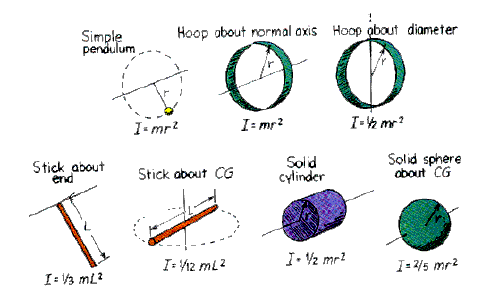
\includegraphics[width=0.8\textwidth]{inertiamoments}
  \caption{Some moments of inertia.\label{fig:inertias}}
\end{figure}

The rotational inertias of several common continuous shapes are given in the following table, and in \cref{fig:inertias}.
\begin{center}
  \def\arraystretch{1.5}
  \begin{tabular}{lll}\hline
    \textbf{Shape} & \textbf{Axis of rotation} & \textbf{Formula}\\\hline
    Hollow cylinder & Along centre & $ I = mr^2 $\\\hline
    Solid cylinder & Along centre & $ I = \frac{1}{2} mr^2 $\\\hline
    Solid cylinder & End point & $ I = \frac{1}{3} mr^2 $\\\hline
    Hollow sphere & Through centre & $ I = mr^2 $\\\hline
    Solid sphere & Through centre & $ I = \frac{2}{5} mr^2 $\\\hline
  \end{tabular}
\end{center}

\begin{example}
  We will derive the formula for the moment of inertia of a solid cylinder of length $ r $ around the end point. Note first
  that we wish to sum up all the little `pieces' of mass $ \dif{m} $; if we take a length of rod $ \dif{\rho} $, then the
  mass of that length is $ \dif{m} = (m/r) \dif{\rho} $. Hence:
  \begin{align*}
    I &= \rint_0^r \frac{m}{r} \rho^2 \dif{\rho}\\
      &= \frac{m}{3r} r^3 = \frac{1}{3} mr^2.
  \end{align*}
\end{example}

\begin{exercise*}
  Use integration to derive the other formulae in the table.
\end{exercise*}

\begin{exercise}
  Racing cyclists use wheels with very light tires and rims. Explain why it is an advantage to reduce the mass of
  the tires and rims rather than the spokes of the wheels.
\end{exercise}

\begin{exercise}
  Which has the larger speed after rolling down the same incline: a sphere, or a hoop (assuming that they have equal radius and mass)?
\end{exercise}

\begin{exercise}
  Suppose we have a thin disc of radius $ R $ and uniform mass $ m $. Let us drop onto it some liquid of density $ \rho $ such that
  the liquid covers the full disc evenly, with a depth $ d $. What is the ratio between the moment of inertia of the original disc
  and the moment of inertia of the disc-liquid system?
\end{exercise}

We can write down a version of Newton's second law for rotational motion (force is resistance to acceleration multiplied by acceleration),
\begin{equation}
  \tau = I \alpha,
\end{equation}
and by recalling that this should be the rate of change of the rotational analogue of momentum and integrating,
we find a formula for \textbf{angular momentum}:
\begin{equation}
  L = I\omega.
\end{equation}
In a closed system, angular momentum is always conserved.

\begin{figure}
  \centering
  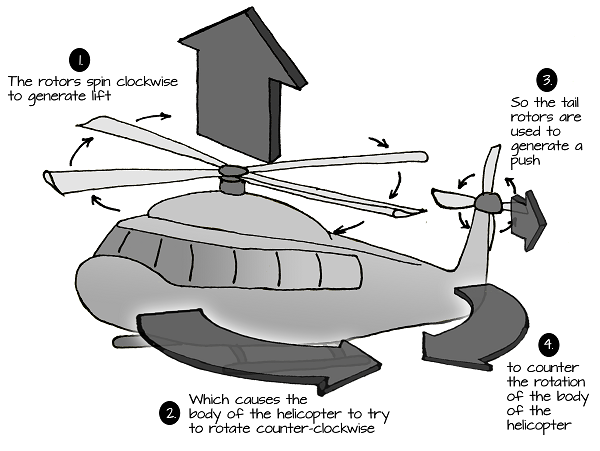
\includegraphics[width=0.7\textwidth]{helicopter}
  \caption{The rotational inertia of a helicopter/rotor system.\label{fig:helicopter}}
\end{figure}

An example of the importance of the conservation angular momentum is the helicopter. When the helicopter is on the ground, it has no angular
momentum. When the rotor begins to turn, there is a tendancy for the helicopter body to rotate in the opposite direction in order to maintain
a net angular momentum of zero; this tendancy must be countered by a tail rotor (\cref{fig:helicopter}).

\begin{exercise}
  A ballet dancer is spinning with arms outstretched. When she pulls her arms into her body, she spins faster.
  Explain this observation.
\end{exercise}

\begin{exercise}
  A helicopter rotor with three blades is rotating at a speed of \SI{529.8}{\rpm}, and has a diameter
  of \SI{7.67}{\metre}. Each blade has a mass of \SI{2.5}{\kilo\gram}. What is the total rotational momentum of the rotor?
\end{exercise}

\begin{exercise}
  A children's merry-go-round in a park consists of an essentially uniform, \SI{150}{\kilo\gram} solid disc rotating around
  a vertical axis. The radius of the disc is \SI{6.0}{\metre}, and a \SI{90}{\kilo\gram} teacher is stading on it at its
  outer edge when it is rotating at \SI{0.2}{\revolution\per\second}. How fast will the disc be spinning if the teacher walks \SI{4.0}{\metre}
  towards the centre along the radius?
\end{exercise}

If a particle of mass $ m $ travelling in a line with constant velocity $ v $ is `captured' into a circular path of radius $ r $,
then it will initially have an angular momentum of
\begin{equation}
  L = mvr = rp.
\end{equation}

\begin{figure}
  \centering
  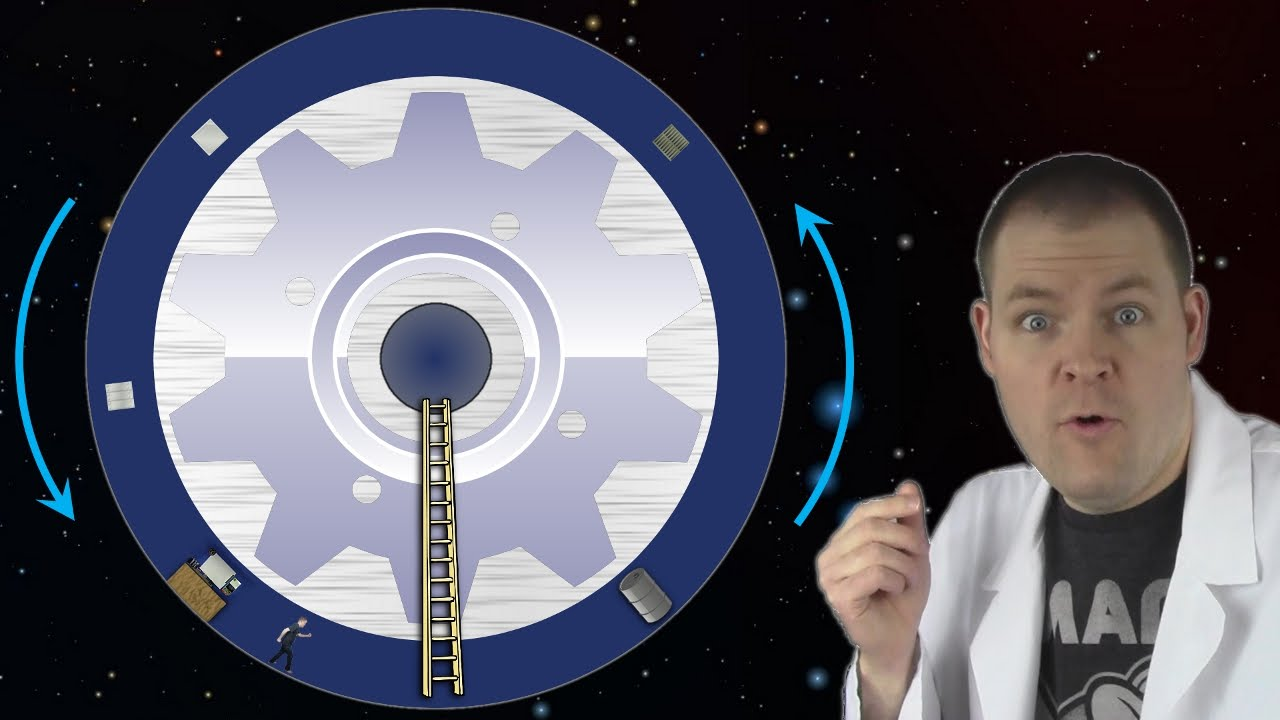
\includegraphics[width=0.7\textwidth]{spinning}
  \caption{A spaceship spinning anticlockwise.\label{fig:spinning}}
\end{figure}

\begin{exercise} [NZQA 2017]
  Sylvia and Sam's spaceship spins anticlockwise on its axis as it is moving through space (\cref{fig:spinning}). The astronauts can change
  the angular velocity of the spaceship by firing two small rockets that are mounted tangentially as shown. The rockets produce a clockwise
  torque. The rotational inertia of the spaceship is \SI{5.80e4}{\kilo\gram\metre\squared}.
  \begin{enumerate}
    \item Calculate the size of the torque required from each rocket to cause an angular acceleration of \SI{2.00e-2}{\per\second\squared}.
    \item The spaceship is rotating anticlockwise at \SI{0.580}{\per\second} when the rockets are fired. Calculate the angular speed of the
          spaceship after one rotation.
    \item Assume that the torque produced by the rockets is constant. Explain what happens to the size of the angular acceleration as the
          rockets gradually emit burnt fuel.
    \item Some time later, the spaceship is rotating freely at \SI{0.450}{\per\second} with the rockets turned off. The spaceship's photo-voltaic
          cells are then extended out from the spaceship, causing the rotational inertia to increase by \SI{2.74e3}{\kilo\gram\metre\squared}.
      \begin{enumerate}
        \item Explain why the period of rotation changes as the cells are extended.
        \item Calculate the period of rotation when the cells are fully extended.
      \end{enumerate}
  \end{enumerate}
\end{exercise}

\section{Rotational Kinetic Energy}
Our final rotational quantity that is analagous to a linear quantity is rotational kinetic energy. Recalling that $ E_k = \frac{1}{2} mv^2 $,
we would guess that the rotational quantity would be given by replacing $ m $ with $ I $ and $ v $ with $ \omega $. This turns out to be
correct:\footnote{~We can also derive this expression by integrating torque over a distance.}
\begin{equation}
  \ekr = \frac{1}{2} I \omega^2.
\end{equation}
We write $ \ekl $ for linear kinetic energy to avoid confusion.

\marginsymbol An interesting problem now presents itself: what is the total kinetic energy of a particle moving around in a circle? Surely if
we just add together the linear kinetic energy and rotational kinetic energy we would be `double-dipping' the velocity somehow?

\begin{exercise}
  Convince yourself that this is not the case (i.e. think of a scenario where an object could have rotational kinetic energy and not
  linear kinetic energy, and vice versa).
\end{exercise}

\begin{example}
  Suppose that a particle of mass $ m $ is moving at a speed $ v $ around a circle of radius $ r $. Then it has linear kinetic
  energy $ \ekl = \frac{1}{2} mv^2 $. Computing its rotational inertia and angular velocity, we obtain $ I = mr^2 $ and $ \omega = v/r $.
  Hence it has rotational kinetic energy $ \ekr = \frac{1}{2} = I \omega^2 = mr^2 (v/r)^2 = mv^2 $!
\end{example}

So, for a point particle, $ \frac{\ekr}{\ekl} = 1 $.

\begin{exercise}
  Consider a spinning uniform disc of mass $ m $ and radius $ R $, moving at a speed $ v $ along a surface due to its spin. Find $ \frac{\ekr}{\ekl} $.
\end{exercise}

\begin{exercise}
  Often, satellites need to be in geostationary orbit: sitting in the atmosphere at a fixed position above a spot on the earth's
  surface. Consider a satellite of mass \SI{1000}{\kilo\gram}.
  \begin{enumerate}
    \item Give a condition on the satellite's angular velocity for this to occur.
    \item Hence calculate the radius of the satellite's orbit.
    \item What is the rotational kinetic energy of the satellite at this point?
    \item How much work must be done to boost the satellite from a low-earth orbit at \SI{300}{\kilo\metre} to a geosynchronous orbit?
  \end{enumerate}
\end{exercise}

\section{Comparison of Linear and Rotational Motion}
\begin{center}
  \def\arraystretch{1.5}
  \begin{tabular}{ccc}
    \textbf{Linear} & \textbf{Concept} & \textbf{Angular}\\\hline
    $ x $ & Displacement & $ \theta $\\\hline
    $ v = \od{x}{t} $ & Velocity & $ \omega = \od{\theta}{t} $\\\hline
    $ a = \od[2]{x}{t} $ & Acceleration & $ \alpha = \od[2]{\theta}{t} $\\\hline
    $ m $ & Inertia & $ I = \sum mr^2 $\\\hline
    $ p = mv $ & Momentum & $ L = I\omega $\\\hline
    $ F = \od{p}{x} = ma $ & Force & $ \tau = \od{L}{\theta} = I\alpha $\\\hline
    $ \ekl = \rint F \dif{x} = \frac{1}{2}mv^2 $ & Mechanical Energy & $ \ekr = \rint \tau \dif{\theta} = \frac{1}{2} I\omega^2 $\\\hline
  \end{tabular}
\end{center}

\chapter{Oscillating Mechanics}
\begin{aquote}{Aristotle}
  Knowledge of the fact differs from knowledge of the reason for the fact.
\end{aquote}

\section{Simple Harmonic Motion}
\begin{figure}
  \centering
  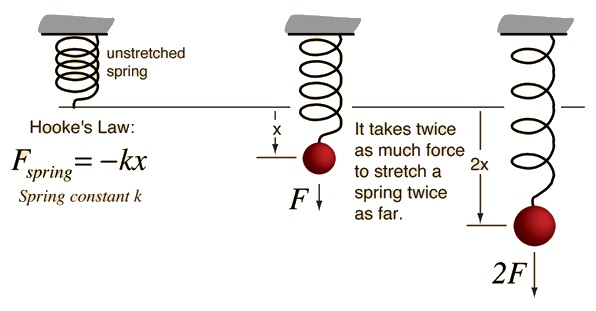
\includegraphics[width=0.7\textwidth]{hooke}
  \caption{Hooke's law is a good basic example of SHM.\label{fig:hooke}}
\end{figure}
There is exactly one force acting on a spring at all times: the restoring elastic force $ F $, which is proportional and opposite to
the displacement $ x $ of the spring (this is Hooke's Law, \cref{fig:hooke}):
\begin{equation}
  F = -kx.
\end{equation}

\marginsymbol Suppose that we want to find the path taken by the end of the spring. We can rewrite the force side of Hooke's Law to be
in terms of the displacement:
\begin{displaymath}
  -kx = F = \od{p}{t} = m \od{v}{t} = m\od[2]{x}{t}.
\end{displaymath}
This is a second-degree differential equation.

\begin{exercise*}
  Show that $ x = A \cos(\sqrt{k/m} \thinspace\cdot t) $ is a solution of the given differential equation.
\end{exercise*}

Now, recall from trigonometry that the general form of a cosine wave is $ x = A \cos(2\pi f t) $. Matching coefficients,
we find that $ 2\pi f = \omega = \sqrt{k/m} $ ($ \omega $ is known as the \textbf{angular frequency}); the frequency of
motion of the end of the spring is
\begin{equation}
  f = \frac{1}{2\pi} \sqrt{\frac{k}{m}}.
\end{equation}

In general, a system which satisfies the condition that the only force acting is proportional to displacement and opposed to
it undergoes motion modelled by a sine wave. This phenomenon is called \textbf{simple harmonic motion} (SHM).

In general, then, a system undergoing SHM with angular frequency $ \omega $ and amplitude $ A $ is modelled by
\begin{equation}
  x = A \cos (\omega t).
\end{equation}

By differentiation, the velocity and acceleration of the system are
\begin{gather}
  v = -\omega A \sin (\omega t), \text{ and}\\
  a = -\omega^2 A \cos (\omega t).
\end{gather}

It directly follows that (why?):
\begin{gather}
  v_\text{max} = \omega A, \text{ and}\\
  a_\text{max} = \omega^2 A.
\end{gather}

\begin{exercise}
  When is the acceleration of a mass undergoing simple harmonic motion greatest? What about the velocity?
\end{exercise}

You should now see that the acceleration is \textbf{in phase} with position, and velocity is exactly \textbf{out of phase}
with position. (What does this mean? Link it back to your experiences with wave motion last year.)

\begin{exercise}
  We showed in \cref{eqn:elenergy} that $ \Delta U_{\ell} = \frac{1}{2} kx^2 $, where $ k $ is the spring constant and $ x $ is the displacement
  of the mass on the spring. If a \SI{2}{\kilo\gram} stationary mass is attached to a spring with spring constant \SI{20}{\newton\per\metre} is
  hit with a hammer and immediately speeds up to \SI{60}{\centi\metre\per\second}, what is the amplitude of its motion?
\end{exercise}

\begin{exercise}
  A \SI{200}{\gram} block attacked to a horizontal spring is oscillating with amplitude \SI{2.0}{\centi\metre} and frequency \SI{2.0}{\hertz}.
  Just as it passes through the equilibrium point towards the right, a sharp blow directed to the left exerts a force of \SI{10}{\newton} for
  approximately \SI{1}{\milli\second}. What is the new amplitude and frequency of oscillation?
\end{exercise}

\section{Pendulums}
\begin{figure}
  \centering
  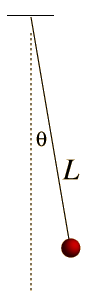
\includegraphics[height=0.25\textheight]{pendulum}
  \caption{Pendulums with small amplitudes can also be modelled by SHM.\label{fig:pendulum}}
\end{figure}
\marginsymbol If a pendulum only swings a small amount, then we can model it as simple harmonic motion. Consider the pendulum pictured
in \cref{fig:pendulum}, where the mass of the string is negligible and the mass of the weight at the end is $ m $. Then
the force of gravity is $ mg $, and the restoring force is $ F = -mg \tan \theta \approx mg \theta $. The displacement $ x $ of the
pendulum end from the central line is given by $ x = L \sin \theta \approx L \theta $; overall, we have that the restoring force is
\begin{displaymath}
  F = -\frac{mgx}{L}.
\end{displaymath}
We now have the same situation as above, with $ k = \frac{mg}{L} $. Hence, we have the following model:
\begin{displaymath}
  x = A \cos\left(\sqrt{\frac{k}{m}} \thinspace\cdot t\right) = A \cos\left(\sqrt{\frac{mg/L}{m}} \thinspace\cdot t\right)
    = A \cos\left(\sqrt{\frac{g}{L}} \thinspace\cdot t\right)
\end{displaymath}
and the frequency is given by
\begin{equation}
  f = \frac{1}{2\pi} \sqrt{\frac{g}{L}}.
\end{equation}

\begin{exercise}
  A pendulum swings in front of a metre ruler. The mass is released from the \SI{24}{\centi\metre} mark and
  takes \SI{0.40}{\second} to move to \SI{86}{\centi\metre} before swinging back.
  \begin{enumerate}
    \item What is the amplitude of the swing?
    \item What total distance along the ruler does the mass move in one complete cycle?
    \item What is the equilibrium position on the ruler?
    \item What is the frequency of the motion?
    \item At the \SI{86}{\centi\metre} mark:
      \begin{enumerate}
        \item Describe the size and direction of the \emph{acceleration} of the pendulum.
        \item Describe the size and direction of the \emph{velocity} of the pendulum.
      \end{enumerate}
    \item At what position will there be no resultant force on the pendulum?
  \end{enumerate}
\end{exercise}

\begin{experiment}
  Make a pendulum and try to figure out how high the maximum displacement of the pendulum
  has to be for SHM to no longer be an accurate predictor of frequency. (You will first need
  to come up with a viable definition of `accurate'.)
\end{experiment}

\begin{figure}
  \centering
  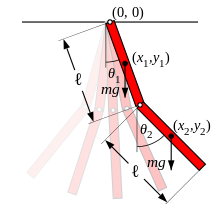
\includegraphics[width=0.4\textwidth]{multipend}
  \caption{A double pendulum.\label{fig:multipend}}
\end{figure}

The physical analysis of double- and triple-jointed pendulums (\cref{fig:multipend}) is much
more complicated (and in the triple-pendulum case almost impossible, due to the chaotic behaviour
that starts to occur).

\goandwatch{https://www.youtube.com/watch?v=dDU2JsgLpm4}

\section{Reference Circles and Phasors}
\begin{figure}
  \centering
  \begin{subfigure}{0.3\textwidth}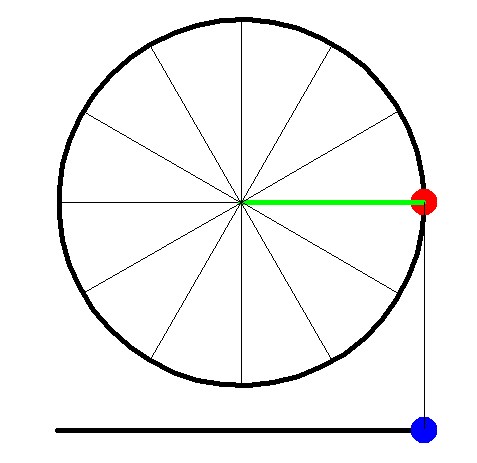
\includegraphics[width = \textwidth]{{shm_animation/frame_00_delay-0.1s}.png}\caption{$ t =  0 $}\end{subfigure}%
  \begin{subfigure}{0.3\textwidth}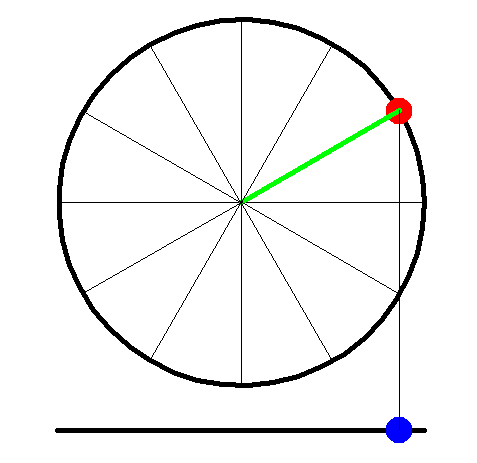
\includegraphics[width = \textwidth]{{shm_animation/frame_01_delay-0.1s}.png}\caption{$ t =  1 $}\end{subfigure}%
  \begin{subfigure}{0.3\textwidth}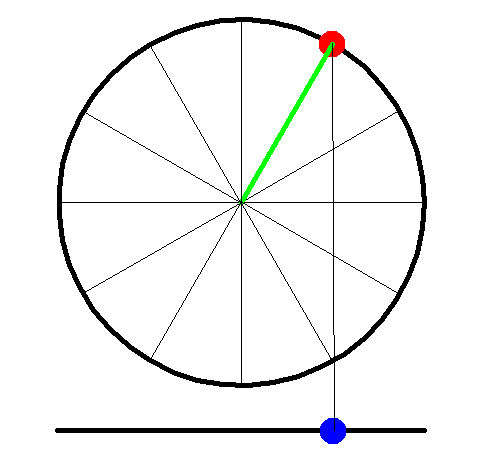
\includegraphics[width = \textwidth]{{shm_animation/frame_02_delay-0.1s}.png}\caption{$ t =  2 $}\end{subfigure}\\%
  \begin{subfigure}{0.3\textwidth}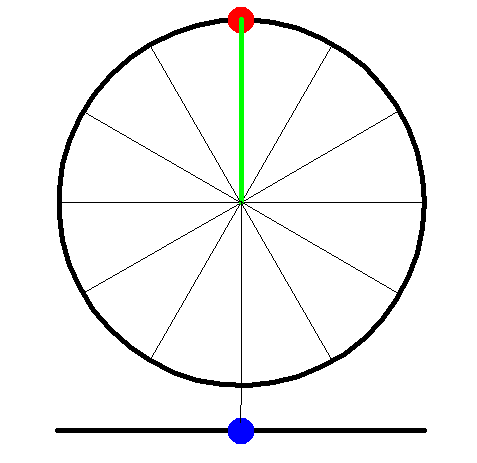
\includegraphics[width = \textwidth]{{shm_animation/frame_03_delay-0.1s}.png}\caption{$ t =  3 $}\end{subfigure}%
  \begin{subfigure}{0.3\textwidth}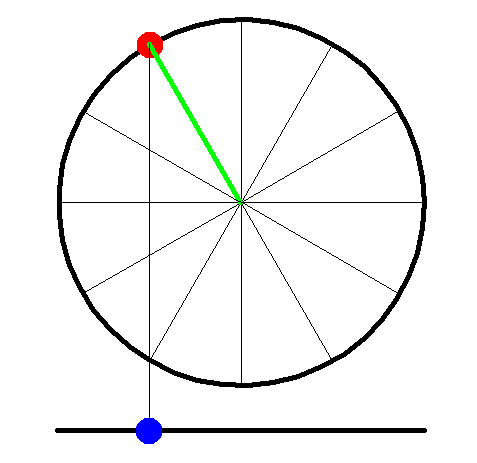
\includegraphics[width = \textwidth]{{shm_animation/frame_04_delay-0.1s}.png}\caption{$ t =  4 $}\end{subfigure}%
  \begin{subfigure}{0.3\textwidth}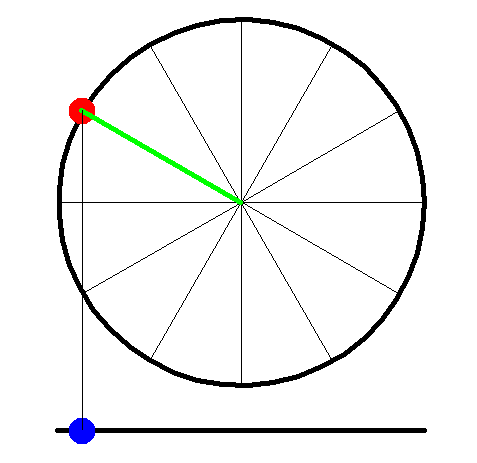
\includegraphics[width = \textwidth]{{shm_animation/frame_05_delay-0.1s}.png}\caption{$ t =  5 $}\end{subfigure}\\%
  \begin{subfigure}{0.3\textwidth}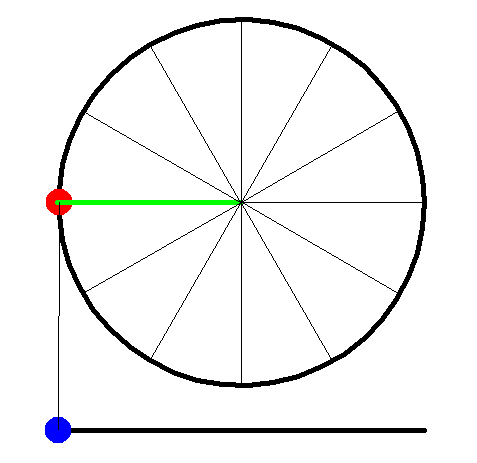
\includegraphics[width = \textwidth]{{shm_animation/frame_06_delay-0.1s}.png}\caption{$ t =  6 $}\end{subfigure}%
  \begin{subfigure}{0.3\textwidth}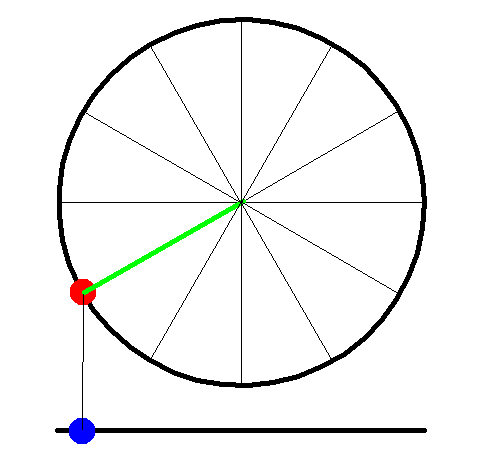
\includegraphics[width = \textwidth]{{shm_animation/frame_07_delay-0.1s}.png}\caption{$ t =  7 $}\end{subfigure}%
  \begin{subfigure}{0.3\textwidth}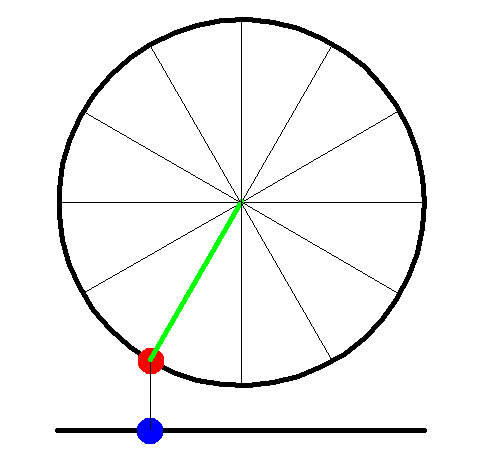
\includegraphics[width = \textwidth]{{shm_animation/frame_08_delay-0.1s}.png}\caption{$ t =  8 $}\end{subfigure}\\%
  \begin{subfigure}{0.3\textwidth}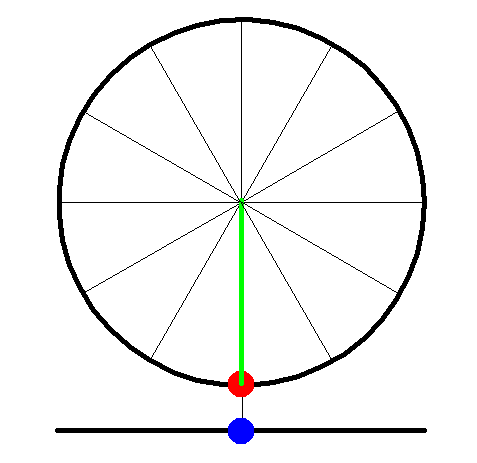
\includegraphics[width = \textwidth]{{shm_animation/frame_09_delay-0.1s}.png}\caption{$ t =  9 $}\end{subfigure}%
  \begin{subfigure}{0.3\textwidth}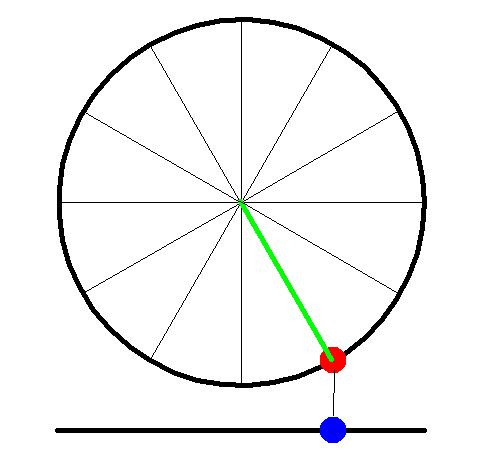
\includegraphics[width = \textwidth]{{shm_animation/frame_10_delay-0.1s}.png}\caption{$ t = 10 $}\end{subfigure}%
  \begin{subfigure}{0.3\textwidth}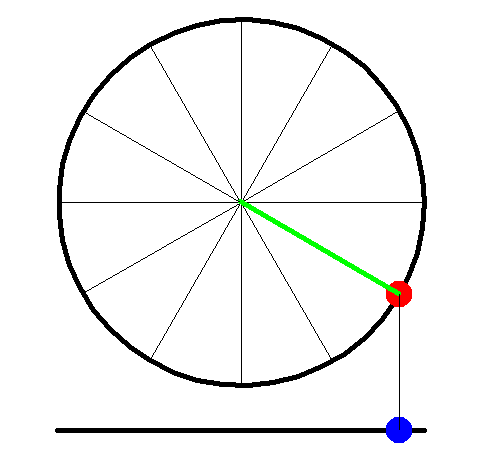
\includegraphics[width = \textwidth]{{shm_animation/frame_11_delay-0.1s}.png}\caption{$ t = 11 $}\end{subfigure}

  \caption{The shadow of uniform circular motion is SHM.\label{fig:shadow}}
\end{figure}

Another view of simple harmonic motion comes from the perspective of uniform harmonic motion. If a particle is moving around a circle
of radius $ r $ with angular velocity $ \omega $, then its shadow will move in simple harmonic motion with amplitude $ r $ (\cref{fig:shadow}).

\goandwatch{https://www.youtube.com/watch?v=d0p7vDIgqjU}

The period of the simple harmonic motion will obviously be $ \frac{2\pi}{\omega} $ and so the frequency will be $ \frac{\omega}{2\pi} = f $;
in other words, the angular frequency of the simple harmonic motion is simply the angular velocity of the particle around the associated
circle.

If we begin with simple harmonic motion of amplitude $ A $ and angular frequency $ \omega $ and then associate a circle with it of radius $ A $,
with a particle moving around the circle at an angular velocity $ \omega $, then that circle is known as the \textbf{reference circle}. The rotating
position vector of the particle is known as a \textbf{phasor}, as it shows the \textbf{phase} of the simple harmonic motion.

In this video, the phasor is the black rotating line; the black particle is undergoing SHM.
\goandwatch{https://www.youtube.com/watch?v=miUchhW257Y}

Obviously, since velocity and acceleration behave 'in the same way' as position in a SHM system, we can draw associated reference circles
and phasors for those too (with the same angular frequency but different amplitudes and phase).

\begin{exercise}
  A bungee jumper free falls for some distance before the cord becomes taut, but after this occurs she undergoes simple harmonic
  motion. For one particular jumper, her angular frequency is \SI{1.8}{\radian\per\second}. On the first descent of her jump, her
  head just touches the water below the bridge she jumped from; after she comes to rest, her head is \SI{3.1}{\metre} above the water.
  During her first bounce:
  \begin{enumerate}
    \item What is the amplitude of her motion?
    \item What is her acceleration at the bottom of the jump?
    \item What is her maximum velocity?
    \item Draw a velocity phasor representing the jumper \SI{0.76}{\second} after she reaches the bottom, and
          hence (or otherwise) calculate her speed at that time.
  \end{enumerate}
\end{exercise}

\textbf{\textcolor{red}{You should take the time to understand phasors now, or you will have an absolute nightmare when we discuss AC electricity later!}}

It is obvious that energy conservation still applies for simple harmonic motion.
\begin{exercise}
  Give an expression for the kinetic energy of a pendulum of mass $ m $ at a time $ t $ after it is released from maximum displacement $ A $.
  Hence find the gravitation potential energy of the pendulum mass three seconds after it is released.
\end{exercise}

The important thing here is that \emph{simple harmonic motion and angular motion are actually the same concept}. Given an oscillating system,
we can find a corresponding rotating system and vice versa.

\begin{exercise}
  A \SI{100}{\gram} mass on a \SI{1.0}{\metre} string is pulled \SI{8}{\degree} to one side and released. How long does it take for the
  mass to reach \SI{4}{\degree} on the other side?
\end{exercise}

\begin{exercise}
  [NZQA 2017] Astronauts need to be able to measure their mass regularly so that they can monitor their health. They can do this by being strapped
  on to a lightweight seat that is attached to a vertical spring. When Sylvia is displaced from equilibrium, she oscillates in simple harmonic motion
  with a period of \SI{8.00}{\second}. You may assume her motion is linear, with an amplitude of \SI{0.120}{\metre}.
  \begin{enumerate}
    \item Use a reference circle or other method to calculate the shortest time it takes for Sylvia to move up \SI{0.080}{\metre} from her
          equilibrium position.
    \item To start the oscillation, Sam applies a vertical force of \SI{4.40}{\newton} to Sylvia. This force causes Sylvia to move a distance
          of 0.120 m. Calculate Sylvia’s mass, describing any assumptions you make to simplify your calculation.
  \end{enumerate}
\end{exercise}

\section{Resonance, Damping, and Driving}
\begin{figure}
  \centering
  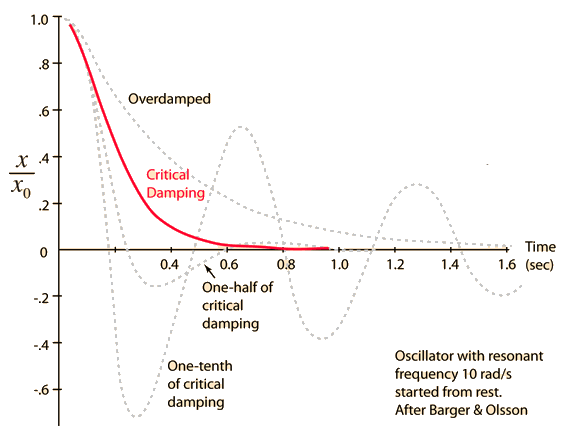
\includegraphics[width=\textwidth]{damping}
  \caption{Different damping scenarios.\label{fig:damping}}
\end{figure}
You will have noticed that pendulums have a \textbf{natural frequency} that they `want' to oscillate at --- it requires
constant attention to prevent them from returning to their more stable frequency. This frequency is the frequency we have
already calculated above: in the case of a spring, it is $ \omega = \sqrt{k/m} $, and in the case of a pendulum it is $ \omega = \sqrt{g/L} $.

In the real world, however, if a pendulum or other oscillating device is left to its own (ahem) devices, then its amplitude of oscillation
will slowly decrease due to the \textbf{damping effect} of friction. The amount of damping (that is, the strength of the damping force) that
causes the amplitude of oscillation to decrease to zero most quickly is called \textbf{critical damping}. If more damping force than this is
applied (the \textbf{overdamped} scenario), then no oscillation occurs and the system returns more and more slowly to equilibrium; if less
force is applied (the \textbf{underdamped} scenario), then the system will oscillate around the equilibrium several times before stopping there.
These phenomena are best seen in a diagram, like \cref{fig:damping}.

In order to counteract damping effects, most real-world systems are \textbf{driven}: an external force is provided to counteract the damping.
This is obviously most effective if the driving force is in phase with the natural frequency of the oscillator.

Fun fact: one of the reasons that aircraft floors are carpeted rather than hard is to dampen the vibration of the floor due to engine or
pump vibration. It is actually possible for the floor panels to resonate if some equipment vibrates at the right frequency, and this is
uncomforable for passengers! (One of the other reasons is that it distributes the load from small-heeled shoes; with just a bare aluminium
or composite floor, it is very possible that a high-heeled shoe could puncture the surface and cause a decompression!)


%%%%%%%%%%%%%%%%%%%%
%%%%%%%%%%%%%%%%%%%%
%%%%%%%%%%%%%%%%%%%%
%%%%%%%%%%%%%%%%%%%%
%%%%%%%%%%%%%%%%%%%%
%%%%%%%%%%%%%%%%%%%%
%%%%%%%%%%%%%%%%%%%%
%%%%%%%%%%%%%%%%%%%%
%%%%%%%%%%%%%%%%%%%%
%%%%%%%%%%%%%%%%%%%%
%%%%%%%%%%%%%%%%%%%%
%%%%%%%%%%%%%%%%%%%%
%%%%%%%%%%%%%%%%%%%%
%%%%%%%%%%%%%%%%%%%%
%%%%%%%%%%%%%%%%%%%%
%%%%%%%%%%%%%%%%%%%%
%%%%%%%%%%%%%%%%%%%%
%%%%%%%%%%%%%%%%%%%%
%%%%%%%%%%%%%%%%%%%%


\swatchcolor{MidnightBlue}
\partcover{wavecover}
\partintro{
  The waves standard this year is mainly an extension of the concepts from Level 2, with an increased focus
  on calculations. Rather than looking at the behaviour of light rays, we focus more on the interference patterns
  of waves with longer wavelengths like sound.

  All of this material should be reasonably straightforward as long as you don't overthink it.
}
\part{Wave Systems}
\chapter{Waves in One Dimension}
\begin{aquote}{Alan Turing}
  We do not wish to penalise the machine for its inability to shine in beauty competitions, nor to penalise a man for losing
  in a race against an aeroplane. The conditions of our game make these disabilities irrelevant.
\end{aquote}
\section{Definition of a Wave}
A \textbf{wave} is an oscillation (vibration) in a medium. The \textbf{amplitude} $ A $
of the wave is the maximum displacement of the medium from its still state; the
\textbf{period} $ T $ of the wave is the length of time taken for one point to complete
exactly one oscillation (i.e. the distance in time between maximum oscillations);
the \textbf{wavelength} $ \lambda $ of the wave is the distance in space at an instant in time
between adjacent points of maximum displacement.

We will assume in this section that waves are uniform (i.e. over a period of time, the parameters
of the wave do not change).

Suppose we wish to find the speed at which the wave appears to move through space.
We know that it will take time $ T $ for a point to change from being maximally displaced
to being minimally displaced and back again; in this time, the wave appears to have moved
forwards exactly one wavelength. Hence the apparent velocity of the wave is
\begin{displaymath}
  v = \od{x}{t} = \frac{\lambda}{T}.
\end{displaymath}
The quantity $ 1/T $ appears often enough that it is given its own symbol $ f $; it is
called the \textbf{frequency} of the wave and measures the amount of times a given point
oscillates up and down per second (or the amount of wavelengths that a wave appears
to move per second). Therefore the \textbf{fundamental wave equation} is
\begin{equation}
  v = f\lambda.
\end{equation}

Since waves vary in time \textit{and} space, we have two equations: one holding our position on
the wave constant, and one holding the time we view the wave constant.

Firstly, the displacement of a single point on a wave at time $ t $ is given by $ y = A\sin(\omega t + \phi) $,
where $ A $ is the amplitude, $ \phi $ is the \textbf{phase} (a measure of the initial position of the particle),
and $ \omega = 2\pi f $ is the \textbf{angular frequency} of the wave.

Secondly, the displacement of each point $ x $ metres along the wave at a given instant is given by $ y = A\sin(\frac{2\pi}{\lambda} t + \phi) $
(or setting $ \nu = 1/\lambda $ to be the \textbf{wavenumber}) $ y = A\sin(2\pi\nu t + \phi) $.

\begin{example}
  Consider a wave of frequency \SI{2}{\hertz} with an amplitude of \SI{2}{\metre}. Initially, a particle on
  this wave  is at a displacement of \SI{2}{\metre} in the positive $ y$-direction. We can therefore derive a description of the
  wave mathematically: $ A = 2 $, $ f = 2 $ so $ \omega = 4\pi $ and we have
  \begin{displaymath}
    y = 2 \sin(4\pi t + \phi).
  \end{displaymath}
  But at $ t = 0 $, $ y = 2 $; so $ 1 = \sin(\phi) $, and $ \phi = \pi/2 $. Hence
  \begin{displaymath}
    y = 2\sin\left(4\pi t + \frac{\pi}{2}\right)
  \end{displaymath}
  is a description of the given point over time.
\end{example}

\begin{exercise}
  The wavefronts of a wave appear to be travelling at a rate of \SI{3.0}{\metre\per\second}; a point which is a
  peak at $ t = \SI{2.0}{\second} $ next reaches maximum displacement again at $ t = \SI{5.0}{\second} $. What is
  the wavelength of the wave?
\end{exercise}

\begin{exercise}
  A particle on a wave oscillates at a frequency of \SI{10}{\hertz} with an amplitude of \SI{0.1}{\micro\metre}. Initially,
  the particle is at a displacement of zero metres from rest. What is the position of the particle after three seconds, and
  in which direction is it moving at that time (in the positive direction or in the negative direction along the $ y$-axis)?
\end{exercise}

\begin{exercise*}
  Find the instantaneous velocity of a given particle on a travelling wave at time $ t = \SI{5}{\second} $ given that its
  maximum displacement from the $ y$-axis is \SI{3}{\centi\metre}, it is initially at position $ y = \SI{2}{\centi\metre} $
  moving upwards (in the positive $ y$ direction), and its period is twenty seconds.
\end{exercise*}

\begin{figure}
  \centering
  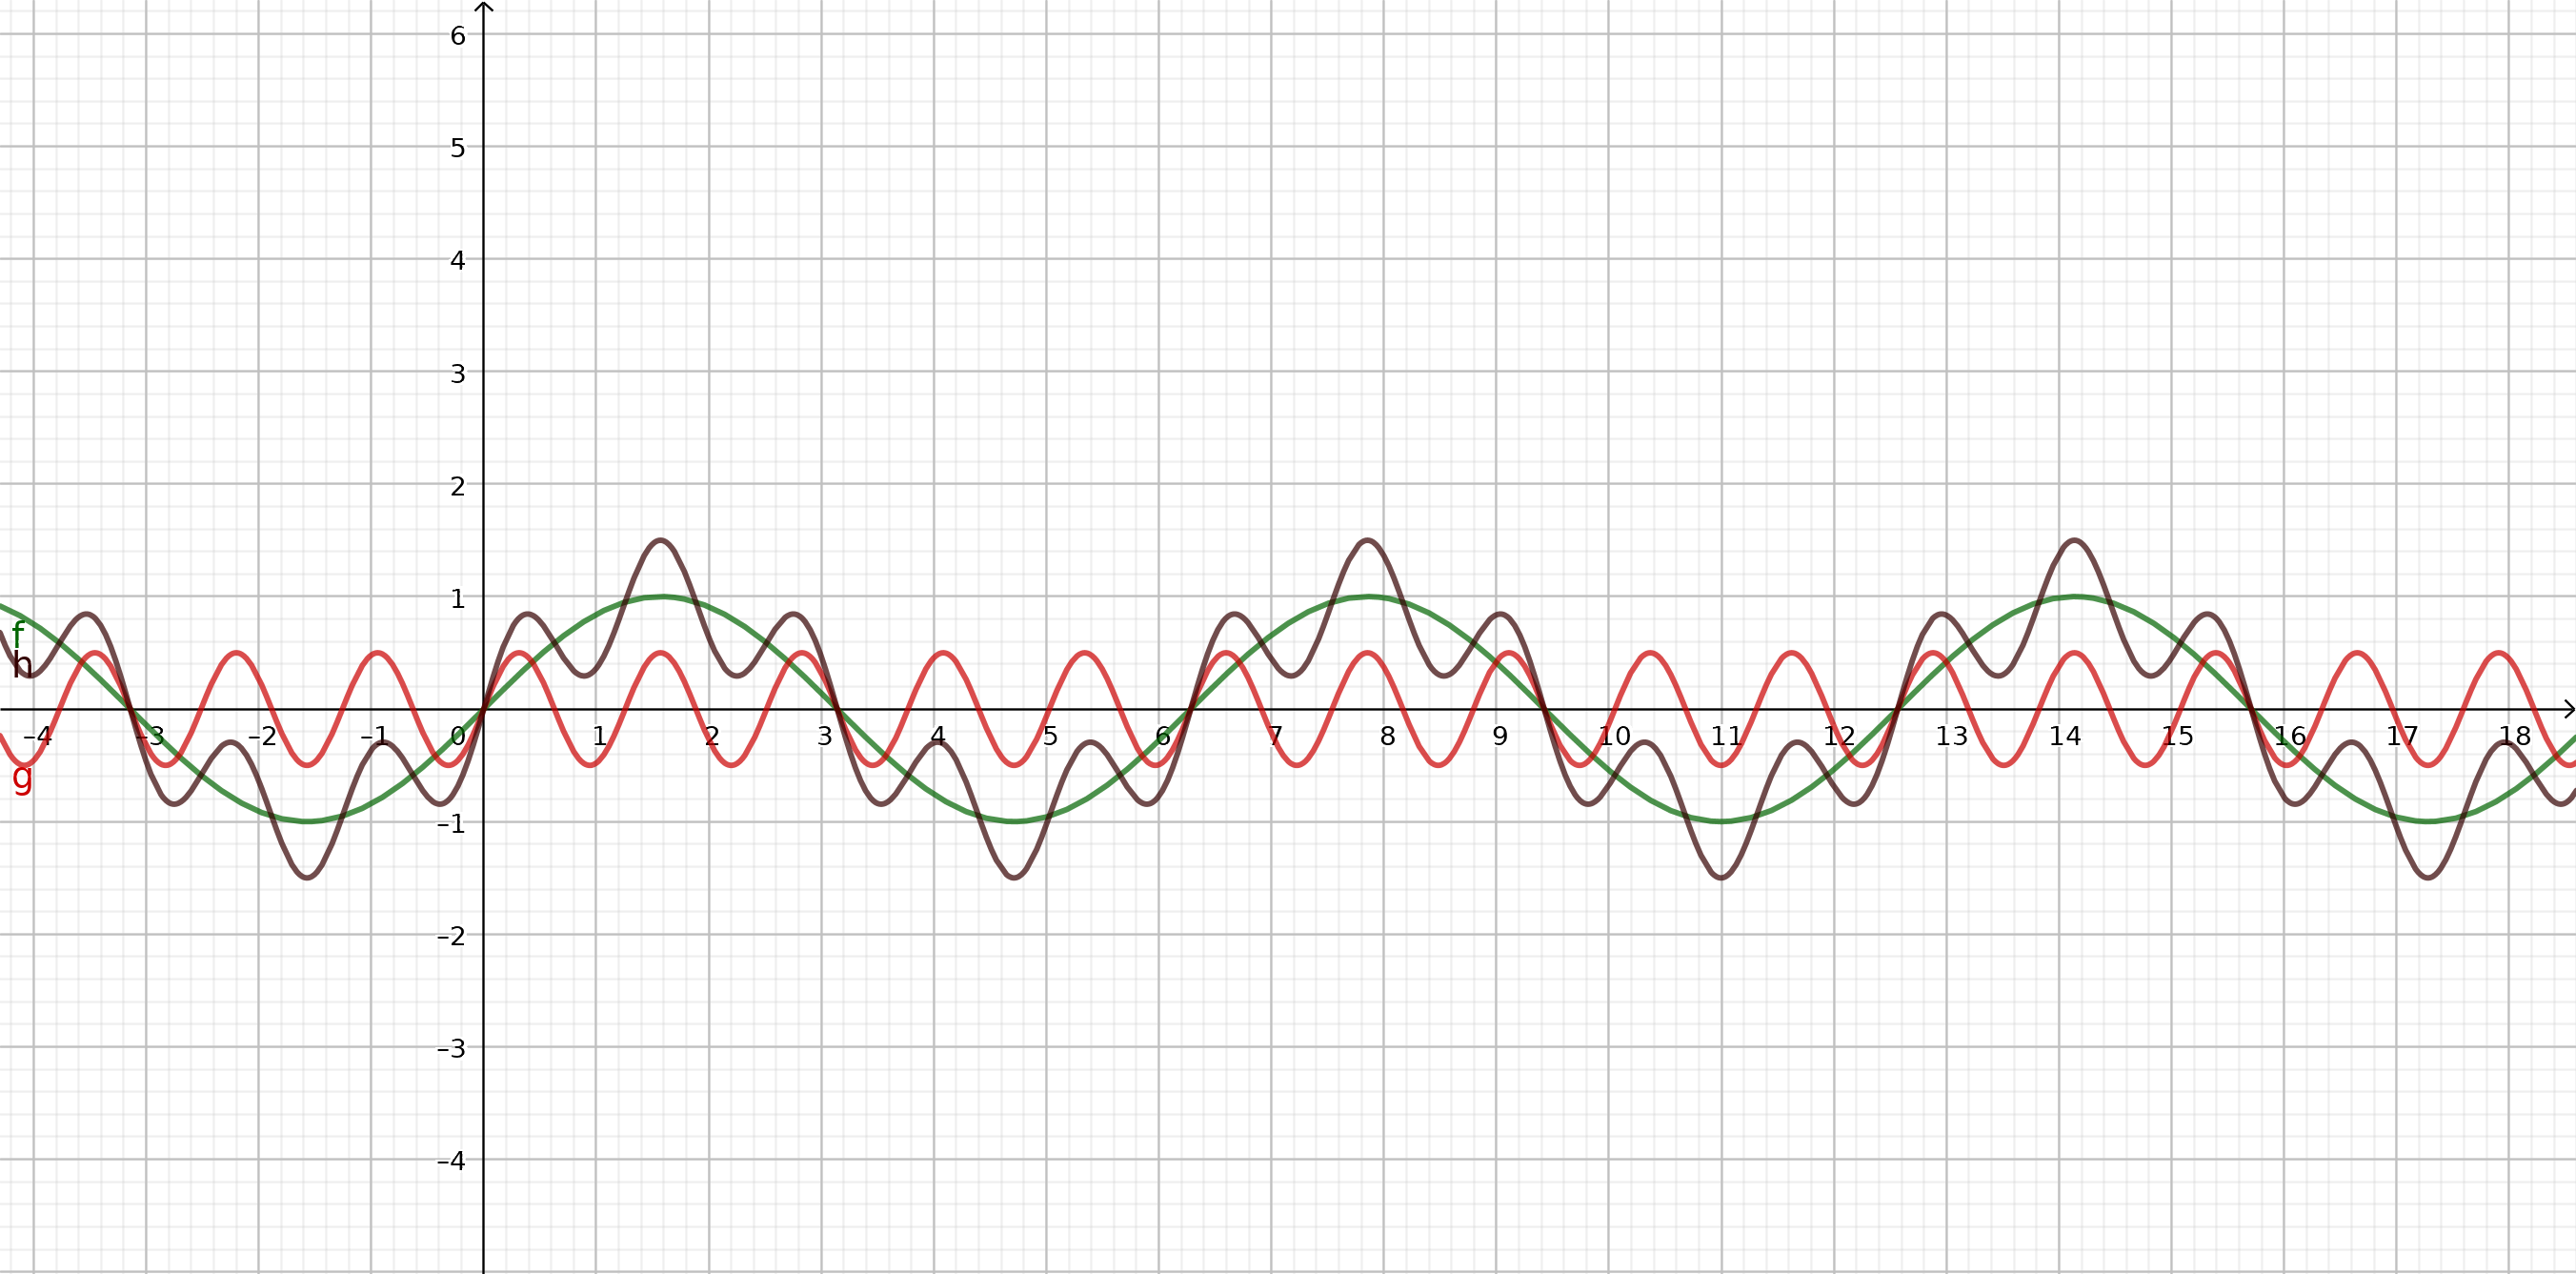
\includegraphics[width=\textwidth]{superposition}
  \caption{The superposition of two waves.}\label{fig:superposition}
\end{figure}
Recall from level two that waves superimpose additively --- that is, if two waves meet then their instantaneous amplitudes at that point
add together. In \cref{fig:superposition}, for example, the green and red waves \textbf{interfere} to produce the black wave.

\section{Standing Waves and Harmonics}
Consider a medium, like a length of string or a column of air, in which two identical waves move in opposite directions. The two
waves will interfere in such a way that no energy is transferred: it is all held stationary, and the wave oscillates up and down
in the medium but the wavefronts do not move. The points where the waves interfere destructively are called \textbf{nodes}, and
the points where maximum constructive interference occurs are \textit{antinodes}. In a standing wave, the wavelength is twice
the distance between adjacent nodes. (Why?)

\goandwatch{https://www.youtube.com/watch?v=no7ZPPqtZEg}

\begin{figure}
  \centering
  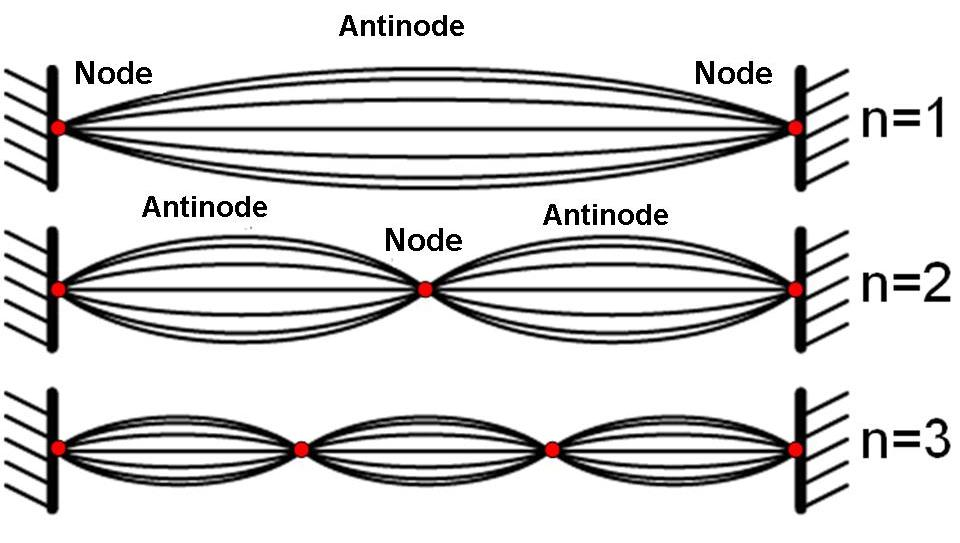
\includegraphics[width=0.7\textwidth]{standingwave}
  \caption{A standing wave on a string.}\label{fig:standingwave}
\end{figure}

Consider a standing wave on a string of length $ L $ where both ends are fixed. The two ends must be nodes, and so $ L $ is an half-integer
number of wavelengths. We write that $ L = \frac{n}{2} \lambda $, where $ n $ is a natural number (1, 2, 3, ...); see \cref{fig:standingwave}.
If $ n = 1 $, the standing wave is known as the \textbf{fundamental standing wave} or the \textbf{first harmonic}. In general, we can
talk about $ n$th harmonics of a medium, where the $ n$th harmonic is the standing wave with $ n $ antinodes.

\begin{exercise}
  Describe one difference between a standing wave and a travelling wave.
\end{exercise}

\begin{exercise}
  A standing wave on a string has three nodes (not including the endpoints). The length of the string is three metres. What
  is the wavelength of the wave?
\end{exercise}

For all values of $ n $, the wave velocity is constant (because it is a property of the medium and not the wave). This implies that only certain
frequencies of waves will produce a standing wave.

\begin{exercise}
  On a string fixed at both ends, a standing wave with one node (not including the endpoints) is induced. The wavelength of
  the wave is \SI{5.00}{\metre}. The speed of a wave in the string is known to be \SI{10}{\metre\per\second}. What is the frequency of the
  fundamental standing wave of the string?
\end{exercise}

\begin{experiment}
  Using a friend, measure the fundamental frequency of a skipping rope (or other type of rope). Use this to calculate the speed
  of a wave in the rope.
\end{experiment}

\begin{exercise}
  Draw the 3rd harmonic of a standing wave in a pipe open at both ends.
\end{exercise}

\begin{figure}
  \centering
  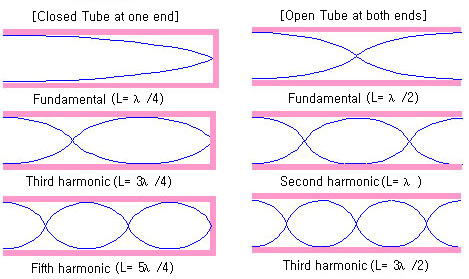
\includegraphics[width=0.7\textwidth]{standingwave2}
  \caption{Standing waves in a pipe.}\label{fig:openpipe}
\end{figure}

In more interesting situations, like a column of air in a pipe, on end of the wave could be an antinode rather than a node (e.g. when the end of
a pipe is open to the air). Refer to \cref{fig:openpipe} to see a diagram of this situation, as well as a situation where both ends of the pipe
are open.

\goandwatch{https://www.youtube.com/watch?v=nR-KXMXpttk}

\begin{exercise}
  A pipe closed at one end is caused to produce its fundamental sound wave of wavelength \SI{3.40}{\metre}. If the velocity of
  sound in air is \SI{340}{\metre\per\second}:
  \begin{enumerate}
    \item Draw a diagram.
    \item Calculate the length of the pipe.
    \item Find the fundamental frequency of the pipe.
    \item Explain why there is no second harmonic.
  \end{enumerate}
\end{exercise}

\begin{figure}
  \centering
  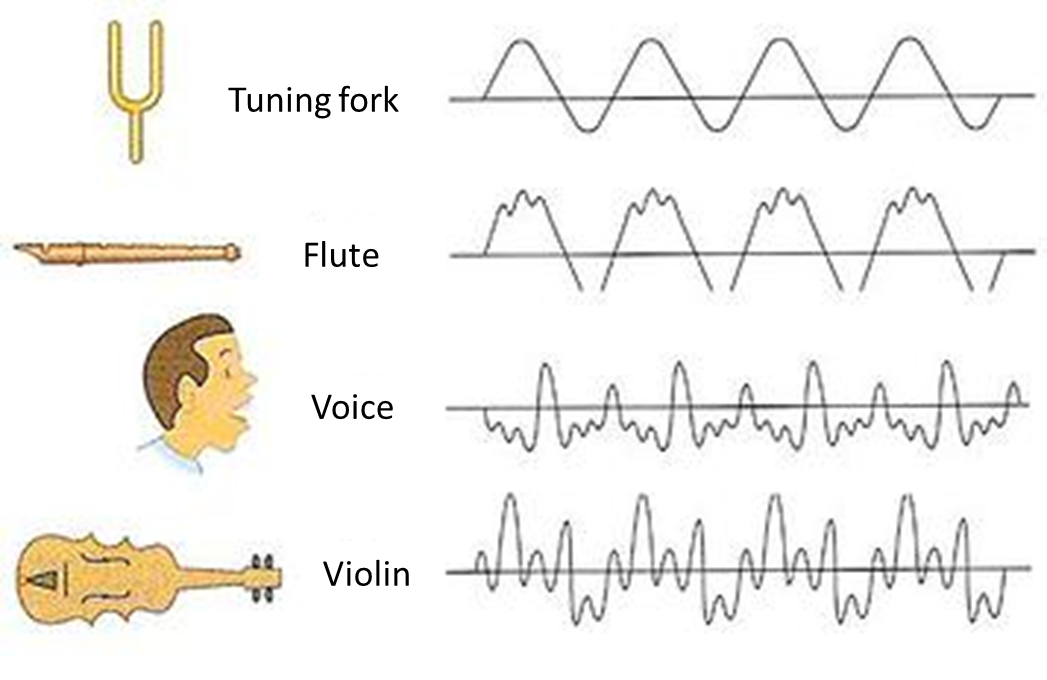
\includegraphics[width=0.6\textwidth]{timbre}
  \caption{These sound sources all have the same fundamental frequency, but different timbre.}\label{fig:timbre}
\end{figure}
Note that in real life, two instruments that are producing the same note still sound different (they have a different \textbf{timbre}). This is
because they produce different combinations of higher harmonics, and the superposition of these harmonics produces a different texture of sound.
For example, \cref{fig:timbre} compares four different sources that are producing the same note but have different sounds due to the different
component waves.


\chapter{Waves in Two Dimensions}
\begin{aquote}{Paul Dirac}
  If there is no complete agreement between the results of one's work and the experiment, one should not allow oneself to be too discouraged.
\end{aquote}
\section{Interference in Two Dimensions}
\begin{figure}
  \centering
  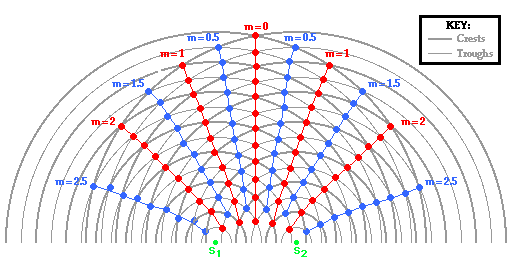
\includegraphics[width=0.7\textwidth]{pathdifference2}
  \caption{Interference in two dimensions.}\label{fig:int2d}
\end{figure}
In two dimensions, waves still interfere. If we have two coherent point sources, like in \cref{fig:int2d}, lines of still medium
will appear where the path difference is a half-integer multiple of the wavelength (the blue lines in the figure) due to total
destructive interference; these lines are \textbf{nodal lines}. Similarly, where the path difference is a full integer multiple
of the wavelength, total constructive interference will occur and we will obtain lines of maximal movement (\textbf{antinodal lines},
red in the figure).

\begin{figure}
  \centering
  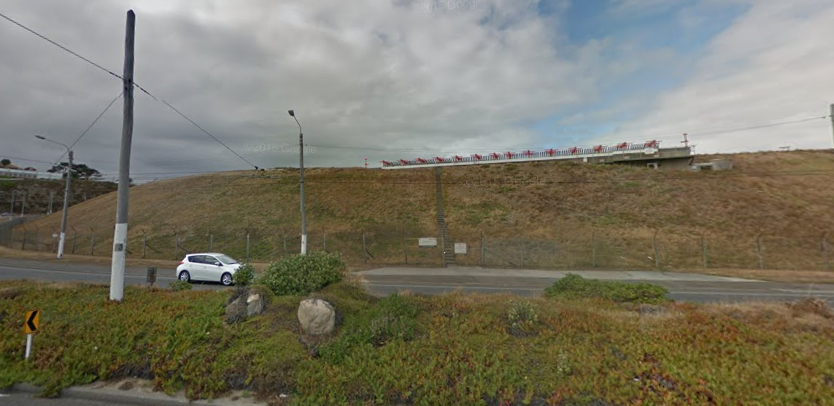
\includegraphics[width=0.7\textwidth]{localiser}
  \caption{The Wellington IFR system at the threshold of runway 16.}\label{fig:localiser}
\end{figure}
\begin{exercise}
  One variety of guidance system for airports involves two radio towers at the end of a runway, one on each side. By modelling
  each as a point source for electromagnetic waves, explain how the aircraft can track the centreline of the runway.
\end{exercise}

\begin{trip}
  More modern systems use a set of side-by-side transmitters, as in \cref{fig:localiser}. This allows the aircraft to determine whether
  it is not only on a correct heading, but also if it is descending at the correct rate. Visit as many other radio-related facilities around
  the airport as legally possible, and determine the role of each (and the physics behind them). As well as the two ends of the runway, there
  are publicly accessible facilities in Strathmore Park (at the end of bus routes 43/44) and at Hawkins Hill (a nice walk from the wind turbine,
  but my preferred route is from a gully on the south coast walkway to Red Rocks that travels over the hills to the south and passes via an old
  military observation post overlooking Cook Strait. Bring a packed lunch and plenty of water.)
\end{trip}

\begin{figure}
  \centering
  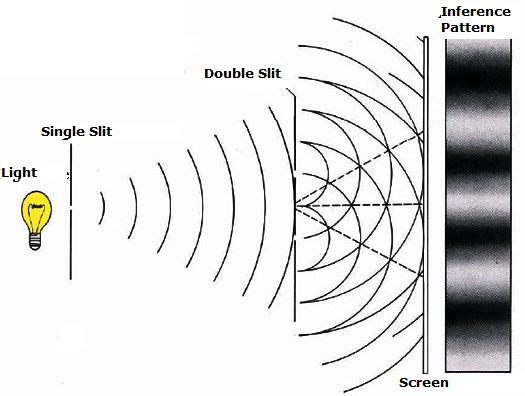
\includegraphics[width=0.5\textwidth]{doubleslit}
  \caption{Young's double slit experiment.}\label{fig:young}
\end{figure}

The result of Young's double slit experiment that we looked at last year (\cref{fig:young}) can be explained using interference --- simply cut \cref{fig:int2d}
with a line parallel to the line joining two slits. (In fact, this effect is seen with particles, like electrons, that are not classically wave-like. This
experiment is one of the first that suggested that classical theories, like those of Newton, would not predict the correct results when lengths become
too small. We explore this in more detail in Part Four.)

\begin{experiment}
  You can carry out Young's experiment yourself --- take a piece of overexposed film and scratch two slits very close to each other, and then shine a laser
  pointer through them onto a piece of paper.
\end{experiment}

\goandwatch{https://www.youtube.com/watch?v=A9tKncAdlHQ}

\begin{figure}
  \centering
  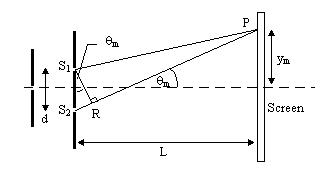
\includegraphics[width=0.5\textwidth]{young3}
  \caption{A diagram of double point-source interference.}\label{fig:young3}
\end{figure}

We can calculate the location of the nodal and antinodal lines as well; consider \cref{fig:young3}, where the two point sources
are $ S_1 $ and $ S_2 $. We want to calculate the position $ y_m $ of the $ m$th patch of constructive interference, as well
as the angle $ \theta_m $.

If $ L >> d $ ($ L $ is much bigger than $ d $), we can assume that $ PS_1 \approx PR $ and that $ \theta_m $ is small. Hence the path difference between the
two rays is the distance $ RS_2 $. Forming a right angled triangle, we have $ RS_2 = d \sin \theta_m $; but for small $ \theta_m $ as in our assumption),
we have $ \sin \theta_m \approx \theta_m $\footnote{~More formally, $ \lim_{x \to 0} \frac{\sin x}{x} = 1 $.} and so $ RS_2 = d\theta_m $. However, for
total constructive interference to occur, this path difference must be an integer multiple of the wavelength; so:
\begin{equation}
  m \lambda = d \theta_m.
\end{equation}

Now turning our attention to calculating $ y_m $, we consider the triangle with base $ L $ and height $ y_m $. Since $ d << L $, the angle of this
triangle at the slit end is approximately $ \theta_m $. We have, therefore, that $ y_m = L\tan \theta_m \approx L \theta_m $, and so:
\begin{equation}
  y_m = L \theta_m = m\frac{L\lambda}{d}.
\end{equation}

\begin{exercise}
  The two formulae given on the NZQA formula sheet are:
  \begin{gather*}
    d \sin \theta = n \lambda\\
    n\lambda = \frac{dx}{L}.
  \end{gather*}
  Compare these with the formulae we have derived, and decide the meanings of $ x $, $ n $, and so on.
\end{exercise}

\begin{exercise}
  Laser light with a wavelength of \SI{635}{\nano\metre} is passed through two slits separated by a distance of \SI{2}{\milli\metre}.
  A screen is placed two metres away from the slits. What is the distance between any two adjacent bright spots on the card?
\end{exercise}

\begin{figure}
  \centering
  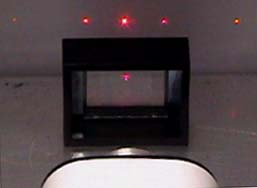
\includegraphics[width=0.5\textwidth]{diffgrating}
  \caption{A laser shining through a diffraction grating.}\label{fig:diffgrating}
\end{figure}
A more complicated situation is that of a \textbf{diffraction grating}, where there are many slits. An interference pattern is produced as
before, but now it covers a much wider area (since the slits are so thin); it has a much larger fringe spacing (due to the small distance
between the slits); and the bright fringes are much brigher (since there are so many slits). A typical pattern is shown in \cref{fig:diffgrating}.

The formula
\begin{displaymath}
  m \lambda = d \sin \theta_m
\end{displaymath}
still applies, but since the fringes are so widely spaced now our angle $ \theta_m $ is not small enough for us to use the small
angle approximation.

\begin{figure}
  \centering
  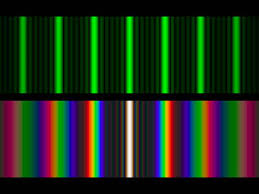
\includegraphics[width=0.5\textwidth]{whitediff}
  \caption{Above: green light shining through a diffraction grating. Below: white light shining through the same grating.}\label{fig:whitediff}
\end{figure}
If we shine white light through a diffraction grating, each frequency of the spectrum is diffracted through a different angle and
so a rainbow of fringes is produced. The difference between shining light of a single colour and white light through the same grating
is displayed in \cref{fig:whitediff}.

\section{Beats}
If two waves of slightly different frequency meet, a regular pulsing of the amplitude of the waves is observed; this phenomenon is
known as \textbf{beating}. The beat frequency $ \tilde{f} $ is related to the frequencies $ f_1 $ and $ f_2 $ of the component waves as follows:
\begin{equation}
  \tilde{f} = \abs{f_1 - f_2}.
\end{equation}

\begin{figure}
  \centering
  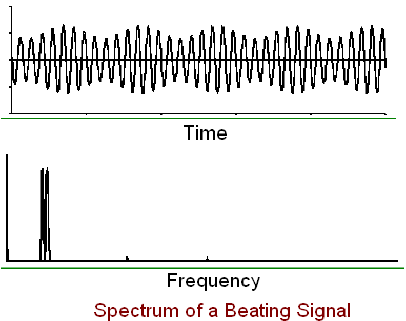
\includegraphics[width=0.5\textwidth]{beats}
  \caption{When two close frequencies sound together, the amplitude of the combined wave oscillates.}\label{fig:beats}
\end{figure}
Consider the situation in \cref{fig:beats}; at the bottom of the diagram, we see a frequency decomposition that tells
us that the wave at the top (which is displaying beats) is formed by the superposition of two waves of incredibly similar
frequency.

\goandwatch{https://www.youtube.com/watch?v=IQ1q8XvOW6g}

\begin{exercise}
  The Queen is listening to the radio in her palace. She has two speakers set up, equally distant from her, but they are
  slightly out of tune. The sound seems to be getting louder and softer periodically. Explain.
\end{exercise}

\begin{exercise}
  A vibrating steel wire on a guitar (of length \SI{0.470}{\metre}) emits a note of frequency $ f_1 $, and
  an open (at both ends) pipe of length \SI{0.530} produces a note of frequency $ f_2 $. The speed of sound in air
  is \SI{340}{\metre\per\second}, and the speed of a wave in the wire is \SI{300}{\metre\per\second}. Find the beat frequency
  produced by the interference of the two waves, if only the fundamental frequencies are produced.
\end{exercise}

Although beating is often annoying, it does have its practical applications. For example, if a tuning fork is known to be
a particular note then the frequency of the beats which it produces when placed next to an untuned instrument can guide
the tuning of that instrument.

\section{The Doppler Effect}
\begin{figure}
  \centering
  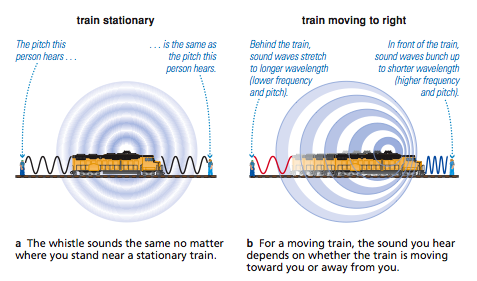
\includegraphics[width=\textwidth]{doppler}
  \caption{A diagram showing the Doppler effect.}\label{fig:doppler}
\end{figure}
\begin{figure}
  \centering
  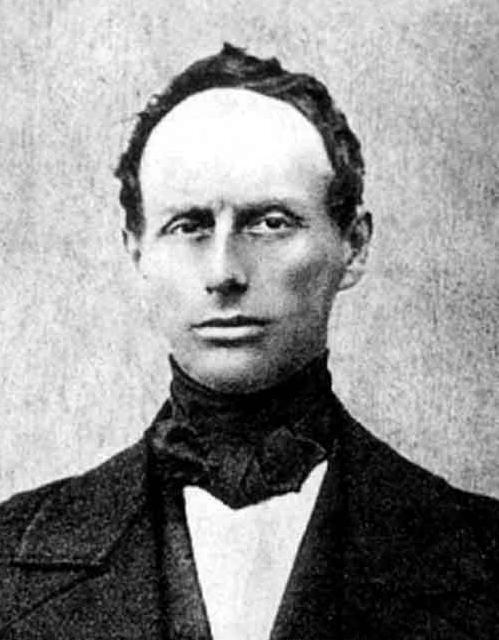
\includegraphics[width=0.5\textwidth]{doppler2}
  \caption{Christian Doppler.}\label{fig:doppler2}
\end{figure}
Consider a stationary observer next to a railway track. If a train sounds its horn while moving towards the observer,
the sound waves will be compressed due to the motion and the observed frequency will be higher than the emitted frequency.
Conversely, if the train is moving away then the waves will be stretched and the observed (apparent) frequency will be lower. This
phenomenon, pictured in \cref{fig:doppler}, is known as the \textbf{Doppler effect} (named for Austrian physicist Christian~Doppler, \cref{fig:doppler2}).

\begin{exercise}
  An ultrasound machine uses reflected sound waves to measure blood flow through a vessel in the body. Explain why we can
  treat the blood cells as wave sources, and hence describe how the machine measures the blood velocity.
\end{exercise}

\marginsymbol Suppose that the wave source, moving towards the observer at a speed of $ v_s $, is emitting waves with a frequency $ f $ and
wave speed $ v_w $. The source emits a wavefront every $ 1/f $ seconds, and in that time the source moves a distance $ v_s/f $. This
is the distance that the \textit{observed} wavelength is diminished by --- so the observed wavelength is $ \lambda - \frac{v_s}{f} = \frac{v_w - v_s}{f} $
and the observed frequency is:
\begin{equation}
  f' = f \frac{v_w}{v_w - v_s}.
\end{equation}
Similarly, if the source is moving away from the observer it can be shown that the observed wave frequency is:
\begin{equation}
  f' = f \frac{v_w}{v_w + v_s}.
\end{equation}

\begin{exercise}
  What if the source is stationary and the observer is moving?
\end{exercise}

\begin{exercise}
  Suppose that the source is moving towards the observer at the speed of sound while emitting a sound
  wave. What will be observed? Hence explain the phenomenon of \textit{sonic booms}.
\end{exercise}

\goandwatch{https://www.youtube.com/watch?v=XmDVvGNtgMg}

\begin{exercise}
  On the Physics Stack Exchange, the user Mark Eichenlaub writes the following about examples of the Doppler effect:
  \textit{I guess one can continue to concoct scenarios. I wonder whether, when you drop a cat off a cliff, you can hear the pitch of
  its screaming drop as it accelerates. (It's not all that cruel --- cats can usually survive a fall at terminal
  velocity.)}\footnote{~Mark Eichenlaub (https://physics.stackexchange.com/users/74/mark-eichenlaub), Doppler effect of sound waves, URL (version: 2014-08-11): https://physics.stackexchange.com/q/9834}

  Conduct an analysis of this scenario. The human ear can hear sounds between \SI{20}{\hertz} and \SI{20 000}{\hertz}, and a cat's scream
  has a frequency of \SI{3000}{\hertz}; at this frequency, a person can determine the difference between two tones if their frequencies
  differ by around 0.3\%. The terminal velocity of a cat is around \SI{97}{\kilo\metre\per\hour}.
\end{exercise}

\section{Waves in Drums}
By applying Newton's laws to a small section of string,\footnote{~See, for example, pages 452-455 of Knight.} it is possible to show that a
1D wave function satisfies the following \textbf{partial differential equation}
\begin{equation}
  \pd[2]{y}{x} = \frac{1}{v^2} \od[2]{y}{t},
\end{equation}
where $ \partial $ (read \textit{dabba}) is used in the derivatives to signify that $ y $ is a function of both time and space. The exact
details of the equation are not important; the main point of introducing it here is to show how we can extend our mathematical models of waves to
higher dimensions. It should be a relatively easy exercise for you to show that
\begin{equation}
  D(x, t) = A\sin(kx - \omega t + \phi_0)
\end{equation}
is a solution to the 1D equation, and that the sum of any two possible solutions is itself a solution.\footnote{~I believe, although I do not want
to check right now, that this exercise is somewhere in my calculus notes.}

Now, the form of these two equations suggest that we can simply `add another dimension' as follows to obtain the general wave equation in 2D:
\begin{equation}
  \pd[2]{z}{x} + \pd[2]{z}{y} = \frac{1}{v^2} \od[2]{z}{t},
\end{equation}
with corresponding solution
\begin{equation}
  D(x, y, t) = A\sin(kx + \ell y - \omega t + \phi_0).
\end{equation}

We can even go to a wave in three dimensions that oscillates in some fourth dimension (perhaps it is an oscillation in the electromagnetic
field rather than a mechanical oscillation) in the obvious way:
\begin{equation}
  \pd[2]{f}{x} + \pd[2]{f}{y} + \pd[2]{f}{z} = \frac{1}{v^2} \od[2]{f}{t}.
\end{equation}
It is my fond hope that you can guess a solution to this based on the hopefully obvious pattern.

\begin{figure}
  \centering
  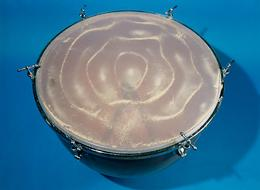
\includegraphics[width=0.5\textwidth]{2dstandingwave}
  \caption{A standing wave on a drum.}\label{fig:2dstandingwave}
\end{figure}
We have already seen too that it is possible to obtain complicated waveforms in 1D by superimposing simpler waveforms (for
example, \cref{fig:superposition}). In 2D, it is possible to obtain even more complicated waveforms; one example which extends
our analysis of wind and string instruments above is that of a drum (\cref{fig:2dstandingwave}). The physical analysis of waves
in a drum is very difficult, due to the chaotic nature of the interactions between the different waves that are created when the drum
is struck. Hitting the drum in a slightly different place may create a significantly different waveform.

\goandwatch{https://www.youtube.com/watch?v=v4ELxKKT5Rw}

%%%%%%%%%%%%%%%%%%%%
%%%%%%%%%%%%%%%%%%%%
%%%%%%%%%%%%%%%%%%%%
%%%%%%%%%%%%%%%%%%%%
%%%%%%%%%%%%%%%%%%%%
%%%%%%%%%%%%%%%%%%%%
%%%%%%%%%%%%%%%%%%%%
%%%%%%%%%%%%%%%%%%%%
%%%%%%%%%%%%%%%%%%%%
%%%%%%%%%%%%%%%%%%%%
%%%%%%%%%%%%%%%%%%%%
%%%%%%%%%%%%%%%%%%%%
%%%%%%%%%%%%%%%%%%%%
%%%%%%%%%%%%%%%%%%%%
%%%%%%%%%%%%%%%%%%%%
%%%%%%%%%%%%%%%%%%%%
%%%%%%%%%%%%%%%%%%%%
%%%%%%%%%%%%%%%%%%%%
%%%%%%%%%%%%%%%%%%%%


\swatchcolor{WildStrawberry}
\partcover{electriccover}
\partintro{
  We continue our study of electromagnetism by looking at the relationships between capacitance, induction,
  and oscillating currents. Circuit analysis (useful for engineering) is also discussed in a little more detail
  than last year. There are some striking links to mechanical systems that we also highlight.

  I think it is important to note that, in my opinion, this is the most difficult of the Level Three topics (and
  may be one of the most difficult of any Level Three paper in any subject). You should have a good grasp of the
  following topics in physics and mathematics:
  \begin{itemize}
    \item Everything in L2 related to electric and magnetic fields
    \item Simple harmonic motion
    \item Definite and indefinite integrals
    \item Differential equations
  \end{itemize}
}
\part{Electrical Systems}
\chapter{DC Circuit Analysis}
\begin{aquote}{Michael Faraday}
  Bacon in his instruction tells us that the scientific student ought not to be as the ant, who gathers merely, nor as the
  spider who spins from her own bowels, but rather as the bee who both gathers and produces. All this is true of the teaching
  afforded by any part of physical science. Electricity is often called wonderful, beautiful; but it is so only in common with
  the other forces of nature. The beauty of electricity or of any other force is not that the power is mysterious, and unexpected,
  touching every sense at unawares in turn, but that it is under law, and that the taught intellect can even now govern it
  largely. The human mind is placed above, and not beneath it, and it is in such a point of view that the mental education
  afforded by science is rendered super-eminent in dignity, in practical application and utility; for by enabling the mind
  to apply the natural power through law, it conveys the gifts of God to man.
\end{aquote}

\section{Kirchoff's Laws}
We begin with a little revision from Level 2. There are two fields (electric and magnetic), which both have associated forces
and therefore associated potential energies. The electric force causes all charges to interact and behaves like gravity (but with
a higher strength); the magnetic force only acts on moving charges.

We have the following law of electromagnetic force (the Lorentz force law):
\begin{equation}
  F = q(E + v \times B).
\end{equation}

\textbf{Current}, the flow of charge, is caused by an electric field in a wire. We define the numerical value of charge to be
\begin{equation}
  I = \od{Q}{t}.
\end{equation}
It can be thought of as the 'amount of electricity' flowing through a cross-section of wire at any instant; it is directly proportional
to the speed and number of electrons (or other charges) flowing.

The \textbf{voltage difference} between two points is the change in potential energy that a unit charge undergoes when moving
between those points. In other words,
\begin{equation}
  V = \frac{\Delta U}{q}.
\end{equation}
Since $ \Delta U = W = F \Delta x = Eq \Delta x $ in a uniform field $ E $ (where $ \Delta x $ is the displacement of the charge), we have
\begin{gather}
  V = E \Delta x \xmapsto{\Delta x \to 0} V = \rint E \dif{x}, \text{ and}\\
  E = -\od{V}{x}.
\end{gather}

In the real world, a conductor has some \textbf{resistance} to the flow of current. The current through a conductor is
directly proportional to the voltage across it by Ohm's law:
\begin{equation}
  I = \frac{\Delta V}{R}
\end{equation}

A conductor whose only purpose is to provide resistance is known as a \textbf{resistor}. If $ R_1 $, $ R_2 $, ... $ R_n $ are in series,
then the total resistance is the sum $ R^* = R_1 + R_2 + \cdots + R_n $; if they are in parallel, then $ R^* = (R_1^{-1} + R_2^{-1} + \cdots + R_n^{-1})^{-1} $.

Resistance causes energy to be dissipated into the environment; the rate of energy dissipation is known (as in mechanics) as power.
\begin{equation}
  P = IV = \frac{V^2}{R} = I^2 R.
\end{equation}

\begin{figure}
  \centering
  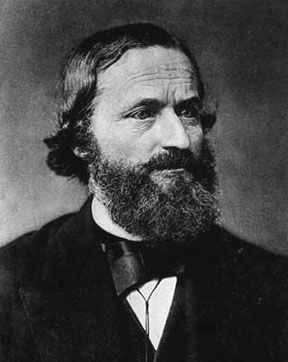
\includegraphics[width=0.5\textwidth]{kirchoff}
  \caption{Gustav Kirchoff.}\label{fig:kirchoff}
\end{figure}

The main laws governing circuits are called \textbf{Kirchoff's laws}, after German physicist Gustav Kirchoff (\cref{fig:kirchoff}). They
are two-fold, and follow from two of the three conservation laws:
\begin{itemize}
  \item (Loop law) Voltage differences around a closed loop add to zero (energy conservation).
  \item (Point law) Currents through a junction add to zero (charge conservation).
\end{itemize}

All \textbf{direct current (DC)} circuits (those where current flows uniformly over time) can be analysed with Kirchoff's laws.

\begin{figure}
  \centering
  \includegraphics[width=0.3\textwidth]{circuit}
  \caption{A circuit with resistors in it.}\label{fig:circuit}
\end{figure}

\begin{example}
  What power is dissipated by the \SI{2}{\ohm} resistor in \cref{fig:circuit}?
\end{example}

\begin{solution}
  We use Kirchoff's loop law to write the following system of equations down (letting $ I_1 $, $ I_2 $, and $ I_3 $ be the currents of the
  three branches from left to right):
  \begin{align*}
    0 &= 12 - 2I_2 - 4I_1\\
    0 &= 12 - 4I_3 + 15 - 4I_1\\
    0 &= 15 - 2I_2 - 4I_3
  \end{align*}

  Solving these simultaneously, we obtain
  \begin{displaymath}
    \begin{bmatrix}
      I_1 \\ I_2 \\ I_3
    \end{bmatrix}
    =
    \begin{bmatrix}
      4.25\\-2.5\\5.0
    \end{bmatrix}
  \end{displaymath}
  and so the power across the \SI{2}{\ohm} resistor is $ P = I_2^2 R = 2.5^2 \times 2 = \SI{12.5}{\watt} $.
\end{solution}

\section{Internal Resistance}
Batteries and other components have an \textbf{internal resistance}; that is, a resistance that is inherently part of the component
and cannot be separated out. This is why batteries and other components heat up during use.

In particular, we can model a battery as a cell together with a resistance:
\begin{center}
  \begin{circuitikz} \draw
    (0,0) to[battery1, l=$\varepsilon$] (2,0) to[R, l=$r$] (4,0);
; \end{circuitikz}
\end{center}

By Ohm's law, $ V_{\text{terminal}} = \varepsilon - Ir $, where $ \varepsilon $ is the \textbf{EMF} of the battery (voltage with no curent)
and $ r $ is the internal resistance.

\begin{figure}
  \centering
  \includegraphics[width=\textwidth]{bushchem}
  \caption{A bush chemist's battery setup.}\label{fig:bushchem}
\end{figure}

\begin{experiment}
  (For chemists.) Using your knowledge of L3 redox reactions, you can make a battery using the following standard electrode potentials:
  \begin{gather}
    \ce{Fe^{2+}(aq) + 2e^- <=> Fe(s)} \qquad E^\circ = \SI{-0.44}{\volt}\\
    \ce{C(s) + 4H^+ + 4e^- <=> CH_4 (g)} \qquad E^\circ = \SI{+0.13}{\volt}
  \end{gather}
  (You can use a non-galvanised nail as the iron source, and lemon juice for the hydronium source (and a graphite pencil works as the carbon electrode in the
  acid). Remember the salt bridge; you can use a coffee filter soaked in \ce{NaOH} solution for this. See \cref{fig:bushchem}.) The theoretical EMF
  of this battery is \SI{0.57}{\volt} (neglecting the formation of iron(III) ions that also occurs). Measure the actual terminal voltage of your battery
  when it is connected across a known resistance, and hence calculate its internal resistance.
\end{experiment}

\section{Capacitance}
\begin{figure}
  \centering
  \includegraphics[width=\textwidth]{ppcapacitor}
  \caption{A parallel-plate capacitor, without (left) and with (right) dielectric.}\label{fig:ppcapacitor}
\end{figure}
A \textbf{capacitor} is a component that stores charge; in some sense, it converts voltage into an electric field. We will begin by considering
a parallel-plate capacitor; that is, a capacitor that consists of two opposing metal plates with charge $ \pm Q $, of area $ A $ and separated
by a distance $ d $ (the left of \cref{fig:ppcapacitor}).

When a capacitor is fully charged:
\begin{itemize}
  \item Electron flow across it stops.
  \item Both plates have equal and opposite charge.
  \item The voltage difference between the plates is the supply voltage.
  \item There is a uniform electric field between the plates.
\end{itemize}

\goandwatch{https://www.youtube.com/watch?v=5qwCmyETAvA}

We find experimentally that the charge $ Q $ on each plate is directly proportional to the voltage difference between them. We
call the constant of proportionality $ C $, the \textbf{capacitance}. The units of capacitance are farads, F.
\begin{equation}\label{eq:capvoltage}
  Q = CV.
\end{equation}

We find that $ C \propto A $, and $ C \propto \frac{1}{d} $. We therefore have the following equation for capacitance of a
parallel-plate capacitor, where the constant of proportionality turns out to be $ \epsilon_0 = \SI{8.85e-12}{\coulomb\squared\per\newton\metre\squared} $
which, you may remember from last year, is called the \textbf{permittivity of free space}:
\begin{equation}
  C = \frac{\epsilon_0 A}{d}.
\end{equation}

\begin{figure}
  \centering
  \includegraphics[width=0.5\textwidth]{dielectric}
  \caption{The effect of a dielectric in a parallel-plate capacitor.}\label{fig:dielectric}
\end{figure}
If we place an insulating material (known as a \textbf{dielectric}) between the plates of the capacitor, the capacitance is observed to
increase. This is because the material is weakly polarised, producing its own electric field that slightly reduces the overall capacitor
electric field (\cref{fig:dielectric}). The capacitance is increased by a factor $ \epsilon_r $ that depends on the specific dielectric but not on the
capacitor that it is placed into: $ C_{\text{with dielectric}} = \epsilon_r C_{\text{without dielectric}} $, or
\begin{equation}
  C = \frac{\epsilon_0 \epsilon_r A}{d}.
\end{equation}

If $ n $ capacitors are placed in parallel, then they act like one large capacitor:
\begin{equation}
  C^* = C_1 + C_2 + \cdots + C_n.
\end{equation}
In series, they tend to reduce the total capacitance:
\begin{equation}
  C^* = (C_1^{-1} + C_2^{-1} + \cdots + C_n^{-1})^{-1}.
\end{equation}
Note that these are the opposite of those for resistors.

\marginsymbol Since there is a potential energy associated with an electric field, the separation of the charges on the opposite plates
of the capacitor means that there is energy stored in the capacitor. The work needed to move an element of charge $ \Delta Q $
from one plate to the other is just $ V \Delta Q $, so the total potential energy stored is $ \rint V \dif{Q} = \rint \frac{Q}{C} \dif{Q} $:
\begin{equation}
  E_C = \rint \frac{Q}{C} \dif{Q} = \frac{1}{2} \frac{Q^2}{C} = \frac{1}{2} QV = \frac{1}{2} CV^2.
\end{equation}

Capacitors resist changes in voltage because it takes time for their voltage to change. If the source voltage across the capacitor
is decreased, it will begin to release energy and so resists the decrease in voltage. Similarly, if the source voltage is increased,
it wil begin to `use up' the extra energy.

\section{Charging and Discharging Capacitors}
\begin{center}
  \begin{circuitikz} \draw
    (0,0) to[opening switch] (2,0) to[C, l=$C$] (2,2) -- (0,2) to[R, l=$R$] (0,0)
; \end{circuitikz}
\end{center}
\marginsymbol Now consider a circuit consisting only of a resistor $ R $ and capacitor $ C $ (an \textbf{RC circuit}). We have that $ V_R + V_C = 0 $;
if the current is $ I $ and the charge on the capacitor is $ Q $, we have $ -IR + \frac{Q}{C} = 0 $.
But the current through the resistor is entirely due to the discharge of the capacitor; so by definition,
we have $ I = -\od{Q}{t} $. Hence
\begin{displaymath}
  \od{Q}{t} R + \frac{Q}{C} = 0
\end{displaymath}
which can be solved via separation of variables:
\begin{align}
  \rint \frac{\dif{Q}}{Q} &= -\rint \frac{\dif{t}}{RC}\nonumber\\
  \ln Q &= -\frac{t}{RC} + C_0\nonumber\\
  Q &= Q_0 e^{-t/RC}.
\end{align}
Note that $ e^{-C_0} = Q_0 $ is the initial charge on the capacitor. We let $ \tau = RC $, and call this the
\textbf{time constant} of the circuit. The time constant is the time taken for the current to reduce to $ 1/e $
of its initial amount; the current is negligible after $ 5\tau $.

Since $ V \propto Q $, we also have
\begin{equation}
  V = V_0 e^{-t/RC}.
\end{equation}

We find an expression for the current by differentiating the charge with respect to time:
\begin{equation}
  I = -\od{Q}{t} = -\od{}{t} Q_0 e^{-t/RC} = \frac{Q_0}{RC} e^{-t/RC} = \frac{V_0}{R} e^{-t/RC} = I_0 e^{-t/RC}.
\end{equation}

The charge and current become negligible after $ t = 5\tau $.

We also have the following equations for charging a capacitor, derived in the same way as those for discharging:
\begin{align}
  Q &= Q_0 (1 - e^{-t/\tau})\\
  V &= V_0 (1 - e^{-t/\tau})\\
  I &= I_0 e^{(-t/\tau)}.
\end{align}

\begin{exercise*}
  Derive the equations for charging a capacitor.
\end{exercise*}

\begin{figure}
  \centering
  \includegraphics[width=\textwidth]{capcharge}
  \caption{The charge/discharge curve for a capacitor.}\label{fig:capcharge}
\end{figure}

See \cref{fig:capcharge} for typical graphs of the charge on a capacitor charging and discharging.

\begin{example}
  The flash on a camera stores energy in a \SI{120}{\micro\farad} resistor that is charged to \SI{220}{\volt}.
  When the flash is fired, the capacitor is quickly discharged through a bulb with \SI{5.0}{\ohm} of resistance.
  \begin{enumerate}
    \item Light from the flash is essentially finished after two time constants have elapsed. For how long does this
          flash illuminate the scene?
    \item At what rate is the lightbulb dissipating energy \SI{250}{\micro\second} after the flash is fired?
    \item What total energy is dissipated by the bulb?
  \end{enumerate}
\end{example}

\begin{solution}\ \\

  (1). We have $ \tau = RC = 5 \times \num{120e-6} = \num{6.0e-4} $ so the flash illuminates the scene
  for approximately $ 2\tau = \SI{0.0012}{\second} $.

  (2).
  \begin{align*}
    P = IV &= I_0 e^{-t/\tau} V_0 e^{-t/\tau}\\
          &= I_0 V_0 e^{-2t/\tau}\\
          &= \frac{V_0}{R} V_0 e^{-2t/\tau}\\
          &= \frac{220^2}{5} e^{-2 \times \num{250e-6}/\num{6e-4}}\\
          &= \SI{4.2e3}{\watt}.
  \end{align*}

  (3). The energy held by the capacitor is $ U = \frac{1}{2} CV_0^2 = 0.5 \times \num{120e-6} \times 220^2 = \SI{2.9}{\joule} $.
\end{solution}

\chapter{Electromagnetic Induction}
\begin{aquote}{James Maxwell}
  This velocity is so nearly that of light, that it seems we have strong reason to conclude that light itself (including radiant
  heat, and other radiations if any) is an electromagnetic disturbance in the form of waves propagated through the electromagnetic
  field according to electromagnetic laws.
\end{aquote}

\section{Basics of Induction}
\begin{figure}
  \centering
  \includegraphics[width=0.8\textwidth]{induction3}
  \caption{A loop of wire being pulled out of a magnetic field. (Diagram modified from 91173 2015)\label{fig:induction3}}
\end{figure}
Recall that \textbf{electromagnetic induction} is the conversion of mechanical energy to electromagnetic energy (i.e. a voltage difference). This
involves a conductor passing through changing magnetic field, which induces a current in in the conductor.

Consider the situation shown in \cref{fig:induction3}, where a wire loop is pulled with a velocity $ v $ out of a magnetic field of strength $ B $.
The voltage $ V $ induced in the loop is given by
\begin{equation}
  V = Bv\ell,
\end{equation}
and the induced current will be anti-clockwise (by the right-hand rule).

\begin{exercise}
  When the loop is entirely within the field and is moved, no current is observed. Explain.
\end{exercise}

Induction is governed by two laws: Lenz's law, and Faraday's law. Rather imprecisely, the two laws taken together state
that \textit{a current is induced in a conductor if and only if the magnetic field through the loop is changing; the direction
of the induced current is such that it produces a magnetic field that opposes the movement inducing the current}.

\section{Magnetic Flux}
\begin{figure}
  \centering
  \includegraphics[width=0.5\textwidth]{weber}
  \caption{Wilhelm Eduard Weber.}\label{fig:weber}
\end{figure}
Before we formally state Faraday's law, we need some kind of concept of the `amount of magnetic field' passing through a given
area. This quantity is known as \textbf{magnetic flux} ($ \Phi_B $), and measured in webers (Wb). The units are named after German
physicist Wilhelm Eduard Weber (\cref{fig:weber}).

\begin{figure}
  \centering
  \includegraphics[width=0.5\textwidth]{flux}
  \caption{Magnetic flux through a surface.}\label{fig:flux}
\end{figure}
If a surface of area $ A $ is perpendicular everywhere to some magnetic field $ B $ (like the situation in \cref{fig:flux}), then the flux
through the surface is given by
\begin{equation}
  \Phi_B = BA.
\end{equation}
More generally, if the field everywhere makes an angle $ \theta $ with the surface, then the flux is given by
\begin{equation}
  \Phi_B = BA \cos \theta.
\end{equation}

Flux is a scalar quantity.

\begin{exercise}
  A flat surface of area \SI{2}{\metre\squared} is parallel to a magnetic field of strength \SI{0.2}{\micro\tesla}. What is the
  magnetic flux passing through the surface?
\end{exercise}

\section{Faraday's Law and Lenz's Law}
We are now in a position to more formally state the laws of induction. Lenz's law tells us about the direction
of the induced current:
\begin{aquote}{Lenz's law}
  An induced current causes a force in opposition to the change creating it --- in other words,
  work must be done against some force in order to induce the current.
\end{aquote}

Faraday's law tells us about the size of the induced current:
\begin{aquote}{Faraday's law}
  The size of an induced voltage around a loop is the rate of change of the magnetic flux within the loop:
  \begin{equation}
    V = -\dod{\Phi_B}{t}
  \end{equation}
\end{aquote}

\begin{exercise}
  A $ \SI{10}{\centi\metre} $ radius circular loop has a total resistance of \SI{0.10}{\ohm}.
  A magnetic field perpendicular to the loop is changing at a constant rate of \SI{-0.3}{\micro\tesla\per\second}.
  What is the current in the loop?
\end{exercise}

\begin{example}
  A $ \SI{20}{\centi\metre} \times \SI{20}{\centi\metre} $ square loop has a total resistance of \SI{0.10}{\ohm}.
  A magnetic field perpendicular to the loop is described by $ B = 4t - 2t^2 $. Compute the current in the loop
  at $ t = 0 $, $ t = 1 $, and $ t = 2 $.
\end{example}

\begin{solution}
  \begin{align*}
    I(t) &= \frac{V(t)}{R} = \frac{1}{R} \abs{\dod{\Phi_B}{t}} = \frac{1}{R} \abs{\dod{}{t} A(4t - 2t^2)}\\
         &= \frac{A}{R} \abs{4 - 4t}\\
         &= \frac{0.04}{0.1} 4\abs{1 - t}\\
         &= 1.6\abs{1-t}.
  \end{align*}
  So $ I(0) = \SI{1.6}{\ampere} $, $ I(1) = \SI{0}{\ampere} $, and $ I(2) = \SI{1.6}{\ampere} $ (in the opposite direction).
\end{solution}

\section{Self-Inductance and the Inductor}
\begin{figure}
  \centering
  \includegraphics[width=\textwidth]{inductors}
  \caption{Various different inductors.}\label{fig:inductors}
\end{figure}
When a switch is closed, it takes time for the current in the circuit to build up from zero. Any coil in the circuit will
then have a changing current through it, and so the magnetic flux in the coil changes --- so, by Faraday's law, there is
an opposing voltage induced.

This phenomenon is known as \textbf{self-inductance}, and a component (like a coil) which produces an opposing voltage when
the current is changed is called an \textbf{inductor}. Since an inductor is often a long coil of wire, the internal resistance is
non-negligible.

This circuit shows the behaviour of a simple circuit when the current begins to increase due to a closing switch.
\begin{center}
  \begin{circuitikz} \draw
    (0,0) to[battery1, l_=$\leftarrow V$] (2,0) to[switch] (3,0) to[R] (3,2) to[L, l_={$\leftarrow$ Opposing voltage.}] (0,2) to[lamp] (0,0)
; \end{circuitikz}
\end{center}

After the inductor has fully `charged' and the switch is opened, the lamp will flash suddenly. This is because the change in current causes an
induced voltage in the coil \emph{in the same direction as the current was flowing}. This induced voltage can even exceed the supply voltage
if the current is changing fast enough. This does not violate Kirchoff's loop law, as there is no longer a closed loop containing the inductor.

We will restrict ourselves now to inductors that are solenoids. If $ \Phi_B $ is the magnetic flux through the core of the solenoid and $ I $ is
the current across it, we find that $ \Phi_B \propto I $. The constant of proportionality, $ L $ is called the \textbf{inductance}:
\begin{equation}
  \Phi_B = LI.
\end{equation}
(Note the similarity to \cref{eq:capvoltage} for capacitors.) The units of capacitance are the henry (H).

If the solenoid consists of $ N $ turns, and has a cross-sectional area of $ A $ and length $ \ell $, then it can be shown that
\begin{equation}\label{eq:physicalinductance}
  L = \frac{\mu_0 N^2 A}{\ell}.
\end{equation}

To compute the potential difference across the inductor, we use Faraday's law:
\begin{equation}\label{eq:inductvolts}
  \Delta V = -\od{\Phi_B}{t} = -\od{}{t} LI = -L \od{I}{t},
\end{equation}
where the negative sign is due to Lenz' law. This formalises the intuitive notion that the induced voltage
would be directly proportional to the rate of change of current.

The power dissipated by the inductor is therefore $ P = IV = LI \od{I}{t} $; recalling that $ P = \od{U}{t} $, we have:
\begin{equation}
  U_L = \rint LI \od{I}{t} \dif{t} = \rint LI \dif{I} = \frac{1}{2} LI^2.
\end{equation}

Compare the behaviour of capacitors and inductors:
\begin{center}
  \begin{tabular}{|c|c|}\hline
    \textbf{Capacitor} & \textbf{Inductor}\\\hline
    Stores energy in an electric field. & Stores energy in a magnetic field.\\
    Damps changes in voltage. & Damps changes in current.\\\hline
  \end{tabular}
\end{center}

We will, later on, answer the natural question: what would happen if you put the two in series?

\section{Inductors in a DC Circuit}
\begin{center}
  \begin{circuitikz} \draw
    (0,0) to[opening switch] (2,0) to[L, l=$L$] (2,2) -- (0,2) to[R, l=$R$] (0,0)
; \end{circuitikz}
\end{center}
Now, we consider a system consisting of an inductor and a resistor (an \textbf{LC circuit}). Suppose that there is a steady current flowing through
this circuit, so that the voltage across the inductor is zero. At some instant $ t = 0 $, let us arrange for the source of
this current to be removed from the circuit without disrupting the system. The inductor will immediately act to produce
a voltage that opposes this dramatic current slope; similarly to the analysis of resistor/capacitor circuits, we find that
\begin{equation}
  I = I_0 e^{-t/(L/R)}.
\end{equation}
let us further define $ \tau = L/R $ to be the time constant of this system, which acts in the same way as the time constant
of a capacitor.

\begin{exercise*}
  Carry out the analysis, in the same way as we did above for capacitors.
\end{exercise*}

For the case where we are charging the inductor, we have
\begin{gather}
  I = I_0 \left(1 - e^{-t/\tau}\right), \text{ and}\\
  V = V_0 e^{-t/\tau}.
\end{gather}

\marginsymbol
\begin{example}
  A 10 turn coil of wire has a diameter of \SI{1.0}{\centi\metre} and a resistance of \SI{0.20}{\ohm}. It is placed in a magnetic field
  of strength \SI{1.0}{\milli\tesla} in a maximum-flux orientation. The coil is connected to an uncharged \SI{1.0}{\micro\farad} capacitor,
  and the magnetic field is switched off. What is the subsequent voltage on the capacitor? (Hint: use $ I = \od{Q}{t} $.)
\end{example}

\begin{solution}
  Model the circuit as a loop consisting of an inductor, a resistor, and a capacitor. We want to find the total charge $Q$ left
  on the capacitor after the inductor finishes discharging, which is the integral $ Q = \rint^\infty_0 I \dif{t} $. This is
  an RC circuit and so the current across the capacitor is given by $ I = I_0 e^{-t/\tau} $, where $ \tau = RC $. However,
  this current also passes through the inductor; the current of the capacitor is given by the same equation, except $ \tau = L/R $.
  Hence $ L/R = RC $ and $ I_0 = \Phi_B/L = \Phi_B/R^2C $. Calculating:
  \begin{align*}
    Q = \rint^\infty_0 I \dif{t} &= \rint^\infty_0 \frac{\Phi_B}{R^2 C} e^{-t/RC} \dif{t}\\
                                 &= \lim_{\alpha \to \infty} \eval{-\frac{\Phi_B}{R} e^{-t/RC}}_{t = 0}^\alpha\\
                                 &= \lim_{\alpha \to \infty} \left[ \frac{\Phi_B}{R} - \frac{\Phi_B}{R} e^{-\alpha/RC} \right]\\
                                 &= \frac{\Phi_B}{R}.
  \end{align*}
  Thus:
  \begin{displaymath}
    \Delta V = \frac{Q}{C} = \frac{\Phi_B}{RC} = \frac{10 \times \pi(\num{0.5e-2})^2 \times \num{1e-3}}{0.2 \times \num{1e-6}} = \SI{3.93}{\volt}.
  \end{displaymath}
\end{solution}

\section{Resonance in a DC Circuit}
\begin{center}
  \begin{circuitikz} \draw
    (0,0) -- (2,0) to[L, l=$L$] (2,2) -- (0,2) to[C, l=$C$] (0,0)
; \end{circuitikz}
\end{center}
\marginsymbol Consider a circuit consisting entirely of an inductor and a capacitor (an \textbf{LC circuit}). As the capacitor
discharges, the current will decrease. This will induce a voltage across the capacitor to resist this decrease in current. By
using Kirchoff's loop law, we have $ V_L + V_C = 0 $. So $ \frac{Q}{C} - L\od{I}{t} = 0 $, and
\begin{displaymath}
  -\frac{Q}{LC} = \od[2]{Q}{t}
\end{displaymath}
(where the negative sign is due to the fact that $ \od{I}{t} $ is the rate of change of current through the inductor,
which is in the opposite direction to the rate of change of charge $ \od{Q}{t} $ on the capacitor). The solution to
this differential equation is
\begin{equation}
  Q = Q_0 \cos \omega t
\end{equation}
where $ \omega = \sqrt{1/LC} $ (check this). Since $ I = -\od{Q}{t} $, we also have
\begin{equation}
  I = -\od{}{t} Q_0 [\cos \omega t] = Q_0 \omega \sin \omega t.
\end{equation}

Hence an LC circuit oscillates with a natural frequency $ \omega $; in an analogy with the mechanical phenomenon of
SHM, $ Q $ corresponds to displacement and $ I $ corresponds to velocity (in some sense). If we add a resistance $ R $,
then this resistance acts as a damping force.

When the current oscillates in this way, it is called \textbf{alternating current}, or AC. We now turn our attention
to studying this kind of current in some detail, and will eventually come back to this similarity between an LC circuit
and resonance.

\goandwatch{https://www.youtube.com/watch?v=Mq-PF1vo9QA}

\begin{exercise}
  Design a practical circuit to measure one second of time accurately.
\end{exercise}

\chapter{AC Circuit Analysis}
\begin{aquote}{Heinrich Hertz}
  It's of no use whatsoever. This is just an experiment that proves Maestro Maxwell was right --- we just have these mysterious
  electromagnetic waves that we cannot see with the naked eye. But they are there.
\end{aquote}

\section{Alternating Current Generators}
\begin{figure}
  \centering
  \includegraphics[width=\textwidth]{acgenerator}
  \caption{An AC generator.}\label{fig:acgenerator}
\end{figure}
Suppose we have a coil of wire rotating in a uniform magnetic field, like \cref{fig:acgenerator}. The induced current will oscillate
from some maximum value $ I_\text{max} $, down to zero, and then reverse until it reaches $ -I_\text{max} $. This device, which tranforms
mechanical (kinetic) energy into an oscillating voltage, is an \textbf{AC generator} and larger versions are used in most power stations
worldwide (the only major power source which does not use such a generator is solar power).

\goandwatch{https://www.youtube.com/watch?v=MW1YUy3Yqpc}

In an ideal situation, the induced voltage at any instant $ t $ is given by
\begin{equation}
  V = V_\text{max} \sin \omega t,
\end{equation}
where $ \omega = 2\pi f = \frac{2\pi}{T} $ is the angular frequency of the system. Since $ I \propto V $, we also have
\begin{equation}
  I = I_\text{max} \sin \omega t.
\end{equation}

\begin{figure}
  \centering
  \begin{tikzpicture}
    \begin{axis}[
      axis lines = center,
      xlabel = $ t $,
      ylabel = $ P $,
      xtick = {0,180,360},
      xticklabels = {$0$, $T/2$, $T$},
      ytick = {0, 0.7071, 1},
      yticklabels = {$0$, rms, max},
      ymajorgrids,
      grid style={line width=.1pt, draw=gray!40}
    ]
      \addplot[domain = 0:360, color = YellowOrange, samples=100] {(sin(x))^2};
    \end{axis}
  \end{tikzpicture}
  \caption{The power output of an AC generator.\label{fig:acpower}}
\end{figure}

We can also think about the power output; since $ P = IV $, the power is given by
\begin{equation}
  P = I_\text{max} V_\text{max} \sin^2 \omega t.
\end{equation}
The power output is graphed in \cref{fig:acpower}.

Since the instantaneous power is oscillating around, it is usually more useful to think about the average power of
the circuit. In this case, the most useful `average' value is the \textbf{RMS (Root-Mean-Square) value}:
\begin{gather}
  I_\text{rms} = \frac{I_\text{max}}{\sqrt{2}}\\
  V_\text{rms} = \frac{V_\text{max}}{\sqrt{2}}
\end{gather}

\textbf{\textcolor{WildStrawberry}{From here, all AC quantities will be given as RMS values unless otherwise stated.}}

\begin{example}
  The voltage across a standard household outlet is \SI{240}{\volt} AC; since this value is RMS, we can calculate the
  peak voltage as $ 240 \times \sqrt{2} \approx \SI{340}{\volt} $.
\end{example}

The definition of the RMS average of a set $ S = \{x_1, x_2, \dots, x_n \} $ of values is given by
\begin{displaymath}
  S_\text{rms} = \sqrt{\frac{1}{n} \left( x_1^2 + x_2^2 + \cdots + x_n^2 \right)};
\end{displaymath}
since we are thinking about a (continuous) function, the sum becomes an integral: the RMS average of a function $ f $ over an
interval $ (a, b) $ is given by
\begin{displaymath}
  f_\text{rms} = \sqrt{\frac{1}{b - a} \rint^b_a [f(x)]^2 \dif{x}}.
\end{displaymath}

\begin{exercise*}
  Given the functions $ I(t) $ and $ V(t) $ defined above, confirm the RMS averages that I stated without proof. Compute
  the RMS value of power in terms of $ P_\text{max} $.
\end{exercise*}

Note that the voltage and current of a circuit with just resistances in it are \textbf{in phase}: the two (probably have different maximum
amplitudes but have the same period and the same initial phase.

\section{Capacitors in an AC Circuit}
Let us consider a circuit consisting of an AC voltage source and a capacitor.

\begin{figure}
  \centering
  \includegraphics[width=\textwidth]{accap}
  \caption{The phase difference between the capacitor voltage and current.}\label{fig:accap}
\end{figure}

\marginsymbol It turns out that there is a \SI{90}{\degree} phase difference between the current and the voltage; in a capacitor-only AC
circuit, the current leads the voltage by \SI{90}{\degree}. To see why, let us look at several instants of the situation shown in \cref{fig:accap}.

\begin{enumerate}[label=\alph*]
  \item The voltage is zero and the capacitor has no charge. The voltage across the capacitor climbs rapidly, leading to the charge on
        the plates of the capacitor increasing rapidly. Close to point b., the voltage is climbing less rapidly and so the current across
        the capacitor decreases.
  \item The voltage instantaneously stops changing, and so there is no current across the capacitor. The source voltage begins to drop again,
        and the capacitor reacts by `losing' some of its charge in the opposite direction as the original current.
  \item Here, the voltage is changing rapidly as it passes through zero. The absolute current is now at a maximum.
  \item The voltage reaches a minimum, and so (as at b.) the current stops since the capacitor is no longer reacting to the changing voltage.
\end{enumerate}

The larger the capacitance, the more charge can accumulate on the plates and so the current must be larger (since the circuit frequency $ \omega $
is unchanged). On the other hand, if we increase the frequency of the voltage source then less time is allowed for the same amount of charge
to accumulate and so in this case the current must be higher as well. This implies that $ I \propto C $ and $ I \propto \omega $, suggesting that
the quantity $ \frac{1}{\omega C} $ acts as an `effective resistance' of the capacitor in an AC circuit. We call this quantity the \textbf{capacitive
reactance}, and give it the symbol $ X_C $. We have the following two relationships:
\begin{gather}
  X_C = \frac{1}{\omega C}, \text{ and}\\
  V_C = I X_C.
\end{gather}
I hope that you can get an intuitive appreciation of this result.

\begin{exercise}
  If a \SI{0.1}{\farad} capacitor is connected to a \SI{15}{\volt} \SI{100}{\hertz} power supply, what is the RMS current through the circuit?
\end{exercise}

Note further that the capacitor current is the same as the current through the voltage source. We have already seen that if we chuck resistors
into an AC circuit then the phase relationships are unchanged, and that the voltage and current of a resistor are unchanged; so the voltage $ V_R $
across the resistive parts of the circuit leads the capacitive voltage $ V_C $ by \SI{90}{\degree}.

Recall from the mechanics topic that in oscillating situations like this we can associate a reference circle and phasor diagram; while it
is kind of unneccessary machinery there, in this particular situation the use of phasors is very useful \emph{as it highlights the phase
relationships between our quantities}!

Throughout this chapter, I will use \textbf{\textcolor{red}{red}} phasors for resistor phase, \textbf{\textcolor{blue}{blue}} phasors
for capacitor phase, and \textbf{\textcolor{OliveGreen}{green}} phasors for inductor phase (yes, it will be getting more complicated). \textbf{Black}
dotted phasors will be reserved for the AC supply. Phasors rotate \emph{anti-clockwise}.

\begin{center}
  \begin{tikzpicture}[scale=3]
    \expphasordeg{0,0}{1}{0}{red,->,ultra thick}
    \expphasordeg{0,0}{0.8}{-90}{blue,->,ultra thick}
    \expphasordeg{0,0}{1.2806}{-45}{black, ->, thick, dotted}

    \draw[fill] (0,0) circle [radius=0.025];
    \node[right] at (1,0) {$V_R$};
    \node[below] at (0,-0.8) {$V_C$};
    \node[below right] at (1,-0.8) {$V_S$};

    \draw[<-, very thick] (0.2,0) arc[x radius=0.2, y radius=0.2, start angle=5, end angle=-355];
%     \path[->, thick] (0.2,0) edge[bend right] (0.2,-0.0000001);
  \end{tikzpicture}
\end{center}

I feel that I should note, even though it is obvious, that the phasors in the diagram \emph{need not} (and usually \emph{will not}) have
the same length.

Now, suppose that we have resistors and capacitors in our little circuit (in series, because I'm not evil); at some instant, the resistors have a
voltage difference across them of $ V_R $ and the capacitors a voltage difference of $ V_C $. If we were looking at a DC circuit, by Kirchoff's loop
law the supply voltage would be $ V_S = V_R + V_C $. However, our voltages are now vectors (I promise that this will make perfect sense one day...),
and so we must use the Pythagorean theorem to add them --- the result,
\begin{equation}
  V_S = \sqrt{\mathstrut V_C^2 + V_R^2},
\end{equation}
is plotted on the phasor diagram above. The angle between $ V_S $ and $ V_R $ is the \textbf{phase difference} between the supply voltage
and the resistor voltage.

Now, we have $ V_R = IR $ and $ V_C = I X_C $, so
\begin{displaymath}
  V_S = \sqrt{I^2 X_C^2 + I^2 R^2} = I\sqrt{X_C^2 + R^2}.
\end{displaymath}
The effective resistance across the source which we have found is called the \textbf{impedance} of the RC circuit; we use the symbol $ Z $
for it, and it has the same units as resistance:
\begin{equation}
  Z = \sqrt{X_C^2 + R^2}.
\end{equation}

\begin{exercise}
  Obtain the same value for $ Z $ by adding together the vectors representing $ X_C $ and $ R $.
\end{exercise}

\begin{exercise}
  Find the impedance of the following circuit:
  \begin{center}
    \begin{circuitikz} \draw
      (0,0) -- (4,0) to[sV, l=$\omega$, a=6\pi<\hertz>] (4,2) to[R, l=$R$, a=10<\ohm>] (0,2) to[C, l=$C$, a=10<\nano\farad>] (0,0)
  ; \end{circuitikz}
  \end{center}
\end{exercise}

Intuitively, thinking of impedance as the `AC version' of resistance will not bring you too many problems this year.

\section{Inductors in an AC Circuit}
Let us now play the same game with an inductor. Consider the simple circuit shown in \cref{fig:acinductor}.

\begin{figure}
  \centering
  \includegraphics[width=\textwidth]{acinductor}
  \caption{The phase difference between the inductor voltage and current.}\label{fig:acinductor}
\end{figure}

In this case, there is also a \SI{90}{\degree} phase difference between the inductive current and the inductive voltage. However,
now the voltage leads the current. To see this, we apply Faraday's law (in the form of \cref{eq:inductvolts}) and use
Kirchoff's law:
\begin{displaymath}
  V - L \od{I}{t} = 0 \implies V = L \od{I}{t}.
\end{displaymath}

\marginsymbol As the voltage across the AC source increases from zero, the voltage across the inductor (caused by the changing magnetic flux through
the inductor core, in turn related to the changing current across the inductor) matches it. At any moment when the voltage is at a maximum
across the inductor, there must be be an increasing current with a large slope; when the voltage is zero then the current should stop changing
and thus be at a maximum; when the voltage is at a minimum (largest negative value), the current must be decreasing quickly. The only model
matching this is that the current acts like a negative cosine wave, while the voltage is a sine wave.

Again, the current through the inductor is the same as the current through any resistance, and so the resistor voltage $ V_R $ must be lagging
behind the inductor voltage $ V_L $ by \SI{90}{\degree}. This is depicted in the following phasor diagram.
\begin{center}
  \begin{tikzpicture}[scale=3]
    \expphasordeg{0,0}{1}{0}{red,->,ultra thick}
    \expphasordeg{0,0}{1}{90}{OliveGreen,->,ultra thick}
    \expphasordeg{0,0}{1.4142}{45}{black, ->, thick, dotted}

    \draw[fill] (0,0) circle [radius=0.025];
    \node[right] at (1,0) {$V_R$};
    \node[above] at (0,1) {$V_L$};
    \node[above right] at (1,1) {$V_S$};

    \draw[<-, very thick] (0.2,0) arc[x radius=0.2, y radius=0.2, start angle=5, end angle=-355];
  \end{tikzpicture}
\end{center}

Inductors also display some effective resistance characteristics like capacitors. If we increase the frequency of the source, there is `less
time' for the voltage to change; if we increase the inductance of the inductor, then we see the same phenomenon. In other words, the effective
resistance of the inductor seems likely to be
\begin{equation}
  X_L = \omega L,
\end{equation}
and this turns out to be correct. We call this quantity the \textbf{inductive reactance}, and it behaves like we would expect:
\begin{equation}
  V = I X_L.
\end{equation}

\begin{exercise}
  \marginsymbol Go back and look at the definitions of $ X_C $ from above, and $ X_L $ here, and convince yourself that they do, in fact,
  behave like resistance in the following ways:
  \begin{itemize}
    \item When reactance increases, the energy stored by the component increases (for a resistor, this would be energy dissipated).
    \item Higher reactance means overall lower current flow through the component.
  \end{itemize}
\end{exercise}

\begin{exercise}
  Show that, in an AC LR circuit, we have
  \begin{gather}
    V_S = \sqrt{V_L^2 + V_R^2}, \text{ and}\\
    Z = \sqrt{R^2 + X_L^2}.
  \end{gather}
\end{exercise}

\section{Resonance in an AC Circuit}
Consider now an LCR circuit, like the following.
\begin{center}
  \begin{circuitikz} \draw
    (0,0) to[L, l=$L$] (4,0) to[sV, l=$\omega$] (4,2) to[R, l=$R$] (0,2) to[C, l=$C$] (0,0)
; \end{circuitikz}
\end{center}

We have all three components to worry about, so our phasor diagram looks like this:
\begin{center}
  \begin{tikzpicture}[scale=3]
    \expphasordeg{0,0}{1}{0}{red,->,ultra thick}
    \expphasordeg{0,0}{1}{90}{OliveGreen,->,ultra thick}
    \expphasordeg{0,0}{0.8}{-90}{blue,->,ultra thick}
    \expphasordeg{0,0}{1.0198}{11.3099}{black,->,thick, dotted}

    \draw[fill] (0,0) circle [radius=0.025];
    \node[right] at (1,0) {$V_R$};
    \node[above] at (0,1) {$V_L$};
    \node[below] at (0,-0.8) {$V_C$};
    \node[above right] at (1,0.2) {$V_S$};

    \draw[<-, very thick] (0.2,0) arc[x radius=0.2, y radius=0.2, start angle=5, end angle=-355];
  \end{tikzpicture}
\end{center}

Again, the supply voltage is the vector sum of the voltages, so we have
\begin{equation}
  V_S = \sqrt{V_R^2 + (V_L - V_C)^2}.
\end{equation}

\begin{exercise}
  Show that the impedance of the circuit is given by
  \begin{equation}
    Z = \sqrt{R^2 + (X_C - X_L)^2}.
  \end{equation}
\end{exercise}

\begin{exercise}
  Suppose that we set up the LCR circuit depicted, with the following parameters:
  \begin{center}
    \begin{tabular}{|cc|}\hline
      $ f $ & \SI{50}{\hertz}\\\hline
      $ L $ & \SI{40}{\milli\henry}\\\hline
      $ R $ & \SI{12}{\ohm}\\\hline
      $ C $ & \SI{100}{\micro\farad}\\\hline
    \end{tabular}
  \end{center}
  Calculate the total reactance of the circuit, the impedance of the circuit, and the phase difference between
  the supply voltage and the current.
\end{exercise}

\begin{figure}
  \centering
  \includegraphics[width=0.5\textwidth]{resonance}
  \caption{The graph of current against frequency for three AC circuits with varying resistance.}\label{fig:resonance}
\end{figure}

Now, suppose that we set up the frequency $ f_0 $ of our circuit such that $ X_C = X_L $. Then we have
\begin{displaymath}
  \frac{1}{2\pi f_0 C} = 2\pi f_0 L
\end{displaymath}
and hence
\begin{equation}
  f_0 = \frac{1}{2\pi \sqrt{LC}}.
\end{equation}

At this frequency, the only factor limiting the current through the circuit is the resistance (why?). It follows
that this frequency will lead to the largest possible currents --- a graph of freqency versus current is shown
in \cref{fig:resonance}.

In this situation, the circuit is said to be \textbf{resonating} or \textbf{tuned}. The frequency $ f_0 $ is called
the \textbf{resonant}, or \textbf{natural}, frequency of the circuit.

\begin{exercise}
  Show that, at resonance, $ V_L = V_C $.
\end{exercise}

\begin{exercise}
  An LCR AC circuit is at resonance; the (RMS) current is measured to be \SI{20}{\milli\ampere}, and the (ideal) inductor
  has a voltage of \SI{20}{\volt} across it. Find the three other voltages ($ V_C $, $ V_R $, and $ V_S $) in the circuit.
  What do you notice about the relative magnitudes of the voltages?
\end{exercise}

In the last exercise, the supply voltage $ V_S $ was \emph{less than} the voltages across the capacitor and the inductor. This
can only occur at (or close to) resonance, and an application of this is given in the next section.

You should also have noticed by now the similarities between LCR circuits (in both AC and DC) and simple harmonic motion.
\begin{center}
  \def\arraystretch{1.5}
  \begin{tabularx}{\textwidth}{|X|X|X|X|}\hline
    & \textbf{LCR Circuit} & \textbf{Pendulum} & \textbf{Spring}\\\hline

    \textbf{Energy changes} & Between storage in the electric field of the capacitor, and the magnetic field of the inductor.
                            & Between kinetic energy and gravitational potential energy.
                            & Between kinetic energy and elastic potential energy.\\\hline
    \textbf{Damping forces} & Resistance in the circuit.
                            & Friction forces.
                            & Friction forces.\\\hline
    \textbf{Driving forces} & The AC supply.
                            & Mechanical forces.
                            & Mechanical forces.\\\hline
    \textbf{Natural\newline frequency} &\rule{0pt}{27pt} $\displaystyle f_0 = \frac{1}{2\pi} \sqrt{\frac{1}{LC}} $
                               & $\displaystyle f_0 = \frac{1}{2\pi} \sqrt{\frac{g}{L}} $
                               & $\displaystyle f_0 = \frac{1}{2\pi} \sqrt{\frac{k}{m}} $\\\hline
  \end{tabularx}
\end{center}

\section{Applications of AC}
\begin{figure}
  \centering
  \includegraphics[width=\textwidth]{westwind}
  \caption{West Wind dumps power onto \SI{110}{\kilo\volt} transmission lines.}\label{fig:resonance}
\end{figure}
\begin{figure}
  \centering
  \includegraphics[width=0.5\textwidth]{transformer2}
  \caption{A typical electronics cabinet on the roadside containing a transformer.}\label{fig:transformer2}
\end{figure}
Most long-distance electricity transmission in New Zealand is done with alternating current rather than direct current.\footnote{~The one
exception is the HVDC link (\SI{350}{\kilo\volt} DC) between Benmore and Haywards underneath the Cook Strait.} This is because, over long
distances, AC is more efficient.

The main way that energy is lost in transmission lines is through the resistance of the conductor. Since $ P = I^2 R $, the energy lost is
proportional to the square of the current. This means that, to minimise the energy loss, we must minimise the current passing through the
wire. However, we still want to be able to transfer large amounts of energy! The solution is to carry electricity at a high voltage (the
voltage between the Brooklyn wind turbine and the substations in Wilton and Central Park is between 110 and 220 \si{\kilo\volt}, and the
voltage on the major transmission line from the Waikato hydro dams to Auckland is \SI{400}{\kilo\volt}), but a low current. Since it is
not practical to deliver tens of thousands of volts to a household socket (the standard wall voltage in New Zealand is \SI{240}{\volt}),
we need an easy way to `step up' and `step down' voltages. This is most easily done with a component known as a \textbf{transformer}, that
only works with AC.

\begin{trip}
  Go and visit the Brooklyn wind turbine and read the information signs at the visitor centre. For bonus points, visit the radar dome
  on top of Hawkin's Hill and revise the waves topic.
\end{trip}

\begin{figure}
  \centering
  \includegraphics[width=\textwidth]{transformer}
  \caption{A simple transformer.}\label{fig:transformer}
\end{figure}

A transformer, like that pictured in \cref{fig:transformer}, consists of two solenoids that share a common core. The changing current
through the \textbf{primary coil} induces a changing magnetic flux in the iron that in turn induces a current in the opposite \textbf{secondary coil}.
This phenomenon is known as \textbf{mutual inductance}.

Now, recall that for a solenoid $ V = -N \od{\Phi_B}{t} $; since the rate of change of flux is the same through each coil, we have
\begin{equation}
  \frac{V_S}{V_P} = \frac{N_S}{N_P}.
\end{equation}

In the real world, transformers are incredibly efficient (up to 99\% efficiency). In order to achieve this efficiency, a number of
design decisions are made:
\begin{itemize}
  \item An iron core is used, since iron has specific properties (related to the particular way the electron shells in iron are filled)
        that mean that magnetic fields within iron are particularly strong.\footnote{~This property is known as \textbf{ferromagnetism}.}
  \item Layers of plastic lamination are used to separate the core into slices, to prevent \textbf{eddy currents} forming.\footnote{~You should have
        studied eddy currents last year in relation to Lenz's law.}
  \item The wire used in the coils is of an extremely low resistance.
\end{itemize}

\goandwatch{https://www.youtube.com/watch?v=vh_aCAHThTQ}

\goandwatch{https://www.youtube.com/watch?v=otu-KV3iH_I}

For an ideal transformer, we have that the power in is equal to the power out; hence we have
\begin{equation}
  V_P I_P = V_S I_S.
\end{equation}

\begin{exercise}
  A particular transformer has a 97\% efficiency. It is used to step down a \SI{240}{\volt} wall socket to
  power a \SI{30}{\volt} appliance that draws an RMS current of \SI{5}{\ampere}. What is the rms current of the
  wall socket?
\end{exercise}

Another application of alternating current is in radio tuners. Consider the following schematic:
\begin{center}
  \begin{circuitikz}
    \draw (0,0) -- (2,0) to[vC, l=$ C $] (2, -3) -- (0, -3) to[L, l=$ L $] (0,0);
    \draw (1,-3) node[ground]{};
    \draw (1, 0) node[antenna]{};
    \draw (2,0) -- (3,0) node[ocirc]{};
    \draw (2,-3) -- (3,-3) node[ocirc]{};
  \end{circuitikz}
\end{center}
The symbol {\ctikzset{bipoles/length=0.4cm}\begin{circuitikz} \draw node[antenna]{}; \end{circuitikz}} is just an antenna (a long length of wire);
the other symbols in the schematic should be familiar (and the output of the radio will be across the two open terminals).

Essentially, the radio is tuned by changing the variable capacitance $ C $ such that the resonant frequency of the tuner circuit matches the
frequency of the radio station that is wanted. If the frequency of the signal matches the resonant frequncy of the circuit, the current will
be driven by this and so will increase. Other frequencies will also be picked up by the antenna, but will not contribute to the resonance of
the circuit and so are not amplified.


%%%%%%%%%%%%%%%%%%%%
%%%%%%%%%%%%%%%%%%%%
%%%%%%%%%%%%%%%%%%%%
%%%%%%%%%%%%%%%%%%%%
%%%%%%%%%%%%%%%%%%%%
%%%%%%%%%%%%%%%%%%%%
%%%%%%%%%%%%%%%%%%%%
%%%%%%%%%%%%%%%%%%%%
%%%%%%%%%%%%%%%%%%%%
%%%%%%%%%%%%%%%%%%%%
%%%%%%%%%%%%%%%%%%%%
%%%%%%%%%%%%%%%%%%%%
%%%%%%%%%%%%%%%%%%%%
%%%%%%%%%%%%%%%%%%%%
%%%%%%%%%%%%%%%%%%%%
%%%%%%%%%%%%%%%%%%%%
%%%%%%%%%%%%%%%%%%%%
%%%%%%%%%%%%%%%%%%%%
%%%%%%%%%%%%%%%%%%%%


\swatchcolor{Plum}
\partcover{moderncover}
\partintro{
  In this topic, we discuss the very small and the very large. Many schools only discuss parts of this standard,
  but it is well worth reading through everything as it is the first time we really enter the 20th century of
  physics.

  We begin with atomic physics and subatomic particles; we then shift gears and talk about relativity, the theory
  introduced by Albert Einstein in the early 1900s that provides a better model for mechanics at high speeds and
  over long distances. Finally, we briefly look at quantum mechanics.
}
\part{Modern Physics}

\bookmarksetup{level=1, keeplevel}
\chapter*{A Word on Pseudoscience}
\begin{aquote}{Gerard 't Hooft\footnotemark}
  You may consider the option of connecting your work with mystery topics such as telepathy and consciousness. Make outrageous claims
  of having solved long standing problems. Of course, you expect that you will become famous, but unfortunately, only a few really good
  theoretical physicists have equations and effects named after them. This is because colleagues recognize their importance and since
  they want to give names to equations and effects anyway, they bestow the discoverers with that honor.  The bad theoretical physicist,
  in anticipation, names his own equations and effects, and even his entire theories, after himself right away.
\end{aquote}\footnotetext{~From \emph{How to become a bad theoretical physicist}, \url{http://www.staff.science.uu.nl/~hooft101/theoristbad.html}}

\begin{figure}
  \centering
  \includegraphics[width=0.9\textwidth]{moon_landing}
  \caption{Most pseudoscience is less sophisticated than moon landing conspiracy theories.}\label{fig:moon_landing}
\end{figure}


Before we start talking about more modern and ``cool'' physics, I feel obliged to take a step
back and remind you that \emph{physics is a science}; that is, physical theories must:
\begin{itemize}
  \item Be based on empirical evidence. Empirical evidence is evidence based on, concerned with, or verifiable by observation or
        experience rather than theory or pure logic.
  \item Make testable, useful predictions.
  \item Be falsifiable --- i.e. it is possible to conceive of an experiment which could prove it wrong.
\end{itemize}

In particular, the following is a non-exhaustive list of pseudoscientific theories (i.e. points of view which do not meet the criteria
above for being scientific theories but are still paraded around as if they were scientific):
\begin{itemize}
  \item `Dianetics' (fails all three criteria, and in addition is championed by that great source of reliable science, the cult of scientology)
  \item `Simulation theory' (does not make testable predictions)
  \item Most things you find on the internet talking about `quantum consciousness' (fails all three criteria)
  \item Intelligent design (not based on empirical evidence, and not falsifiable)
  \item Cryptozoology (not based on empirical evidence)
  \item Ufology (not based on empirical evidence)
  \item The `2012 phenomenon' (not based on empirical evidence, especially as the year is now 2017 and the universe is still in existance)
  \item Homeopathy (not based on empirical evidence)
\end{itemize}
I have intentionally named these examples without description, as I believe that it is really a waste of space to discuss them. Unfortunately,
pseudoscientific theories are becoming easier to find (by means of the internet), and most of them just want your money --- by all means research
them on your own, but there are better things to spend your time on.

When researching the topics we are about to discuss on your own, take care that you:
\begin{enumerate}
  \item Ensure that the resources you use reference actual, repeatable experiments that have been (or could conceivably be) performed; and
  \item Are not `too good to be true'.
\end{enumerate}

Some reputable physics sources on YouTube include the Fermilab channel (popular videos by physicist Don Lincoln), the Royal Society channel, and
lectures by physicists like Brian Cox.

\begin{figure}
  \centering
  \includegraphics[width=0.7\textwidth]{pseudoscience}
  \caption{Psst... do you have a moment to talk about the space yeti?}\label{fig:pseudoscience}
\end{figure}

\chapter{Atomic Physics}
\begin{aquote}{Richard Feynman}
  Energy is a very subtle concept. It is very, very difficult to get right.
\end{aquote}

\section{Historical Models of the Atom}
\begin{figure}
  \centering
  \begin{subfigure}{0.4\textwidth}
    \includegraphics[width = \textwidth]{einstein}
    \caption{Albert Einstein. \label{fig:einstein}}
  \end{subfigure}\hfill%
  \begin{subfigure}{0.4\textwidth}
    \includegraphics[width = \textwidth]{perrin}
    \caption{Jean Perrin. \label{fig:perrin}}
  \end{subfigure}%
  \caption{The two physicists who used Brownian motion to verify the atomic hypothesis.}
\end{figure}

The word \textit{atom} comes from the Greek \textgreek{ατομος} `atomos', meaning indivisible. The first model of the atom, as
an indisible bit of matter, was described by the Greek philosphers Leucippus and Democritus in the 5th century BCE. Until the
19th century, scientists were unable to test the various competing models of matter; in the early 1800s, chemist John Dalton
used atomic theory as the explanation of the fact that chemicals always react in ratios of whole numbers, and by the start of
the 20th century the idea of small units of matter was generally accepted within the scientific community as a result of work
done by Albert Einstein (a German-born physicist, \cref{fig:einstein}, who undertook a study of the random motions of particles
floating on water and theorised that they were due to the movement of small units of matter) and Jean Perrin (a French
physicist, \cref{fig:perrin}, who won the Nobel Prize in Physics in 1926 for his verification of Einstein's predictions).

\begin{figure}
  \centering
  \includegraphics[width=0.5\textwidth]{thomson}
  \caption{J.J. Thomson. \label{fig:thomson}}
\end{figure}
\begin{figure}
  \centering
  \includegraphics[width=\textwidth]{crt}
  \caption{Thomson's experiment to detect electrons. \label{fig:crt}}
\end{figure}
\begin{figure}
  \centering
  \includegraphics[width=0.4\textwidth]{pudding}
  \caption{The plum pudding model of the atom. \label{fig:pudding}}
\end{figure}
In 1897, J.J. Thompson (an English experimental physicist, \cref{fig:thomson}) deflected cathode rays --- generated by applying a
voltage across two electrodes in a vacuum tube --- using a magnet (\cref{fig:crt}), and so showed that they were made up of small
negatively charged particles about 1800 times lighter than the hydrogen atom. We now call these particles \textbf{electrons}. This
was the first scientific observation of quantities of matter smaller than the atom. Thomson conjectured, based on his experiments,
that an atom was made up of electrons distributed throughout a uniform custard of positive charge. This model of the atom (\cref{fig:pudding})
is known as the \textbf{plum pudding} model.

\begin{figure}
  \centering
  \begin{subfigure}{0.4\textwidth}
    \includegraphics[height = 0.3\textheight]{geiger}
    \caption{Hans Geiger. \label{fig:geiger}}
  \end{subfigure}\hfill%
  \begin{subfigure}{0.4\textwidth}
    \includegraphics[height = 0.3\textheight]{marsden}
    \caption{Ernest Marsden. \label{fig:marsden}}
  \end{subfigure}%
  \caption{The two physicists who performed an experiment that discovered the existence of the atomic nucleus. \label{fig:geigerandmarsden}}
\end{figure}
\begin{figure}
  \centering
  \includegraphics[width=0.4\textwidth]{ruthmodel}
  \caption{The Rutherford model of the atom. \label{fig:ruthmodel}}
\end{figure}
In 1909, New Zealander Ernest Rutherford directed Hans Geiger and Ernest Marsden (\cref{fig:geigerandmarsden}) in an experiment
that involved firing helium nuclei ($\alpha$-particles) at gold foil to observe the scattering patterns. Based on Thomson's model,
it was expected that most of the particles would pass straight through with little deflection. However, it was observed that some
particles ricocheted backwards, which was impossible according to the plum pudding model, and suggested that the positive charge
of the atom is concentrated in a small \textbf{nucleus} at the centre of the atom, surrounded by electrons. This model is known
as the \textbf{Rutherford} model of the atom (\cref{fig:ruthmodel}).

By 1913, the Rutherford model was found to be inadequate as it did not explain why the electrons, who are continually accelerating (due
to their orbit) and so are burning energy, do not `fall in' towards the nucleus. It also did not explain why atoms only absorb or emit
radiation of specific frequencies.

\begin{figure}
  \centering
  \includegraphics[width=0.4\textwidth]{bohr}
  \caption{Niels Bohr. \label{fig:bohr}}
\end{figure}
\begin{figure}
  \centering
  \includegraphics[width=0.5\textwidth]{bohratom}
  \caption{Bohr's model of the atom, with quantised electrons. \label{fig:bohratom}}
\end{figure}
\marginsymbol To fix these problems, the German physicist Niels Bohr (\cref{fig:bohr}), together with Rutherford, postulated that the orbits of
electrons are \textbf{quantised}: that is, electrons can only have certain discrete energies when orbiting the nucleus and so will
form `electron shells'. This model is known as the \textbf{Bohr} model of the atom (\cref{fig:bohratom}).

The Bohr model has since been superceeded by a quantum-mechanical view of the atom, which intuitively consists of a `probability
cloud' around the nucleus that predicts where it is most likely to find the electrons at each point in time (\cref{fig:allmodels}).
However, since the Bohr model is more intuitive and is correct in most of its predictions that we are interested in for this first
section, it is the one that we will focus on.

\begin{figure}
  \centering
  \includegraphics[width=\textwidth]{allmodels}
  \caption{All the historical models of the atom, up to the present. \label{fig:allmodels}}
\end{figure}

\section{The Photoelectric Effect}
\begin{figure}
  \centering
  \includegraphics[width=0.5\textwidth]{hertz}
  \caption{Heinrich Hertz. \label{fig:hertz}}
\end{figure}
Heinrich Hertz (\cref{fig:hertz}), a German physicist, observed an interesting phenomenon in 1887: when light strikes a metal surface, electrons
are emitted. This is known as the \textbf{photoelectric effect}.

When UV light falls on a sheet of metal, its energy is absorbed and some is transferred to electrons which are ejected as fast-moving particles
(\textbf{photoelectrons}). A certain amount of energy must be transferred to an electron before it can be emitted; this amount is dependent on
the type of metal and is known as the \textbf{work function} $ \phi $ of the metal. This energy is quite small in absolute terms, and can easily
be provided by electromagnetic waves. However, some observations surrounding the photoelectric effect cannot be explained by treating light as a
wave, and seem to suggest that light in fact acts as a particle!

\begin{center}
  \def\arraystretch{1.5}
  \begin{tabular}{|p{0.4\linewidth}|p{0.4\linewidth}|}
    \hline
    \textbf{Predicted by the wave theory} & \textbf{Observed phenomena}\\\hline
    A brighter light would cause electrons to have greater kinetic energy when released. &
    Brighter light caused \textbf{more} electrons of the \textbf{same} kinetic energy to be released.\\\hline
    If a dim light were used, electrons would need to accumulate energy to overcome the work function and so would not be emitted instantaneously. &
    When UV light was used, even the faintest light caused instant electron emission.\\\hline
    The frequency of light would not cause any change in observations. &
    A higher frequency of light caused electrons to have a higher kinetic energy. Below a certain frequency,
    no electrons were emitted.\\\hline
  \end{tabular}
\end{center}

On the other hand, from experiments like Young's double-slit experiment, we know that light can sometimes act as a wave (\cref{fig:young})! In order
to reconcile these two viewpoints of light, we need to extend our ideas of quantisation from the energies of the atom to the energies of light.

\begin{figure}
  \centering
  \includegraphics[width=0.5\textwidth]{planck}
  \caption{Max Planck. \label{fig:planck}}
\end{figure}
Albert Einstein proposed in 1905, building off the ideas of Max Planck (\cref{fig:planck}), that electromagnetic radiation comes in packets (\textbf{quanta}) of
fixed size known as \textbf{photons}; the energy of an individual photon is directly proportional to the frequency of light, with a constant
of proportionality $ h \approx \SI{6.63e-34}{\joule\second} $ known as \textbf{Plank's constant}. In other words, the energy of a photon is given by:
\begin{equation}
  E = hf.
\end{equation}
It is interesting that here in the microscopic world a particle's energy is related to the \emph{frequency} rather than its associated wave amplitude.

If we apply this to the photoelectric effect, we can calculate that the energy of emitted photoelectrons
when light of frequency $ f $ is incident on a metal with work function $ \phi $ is given by
\begin{equation}
  E = hf - \phi.
\end{equation}

This allows us to calculate the \textbf{critical frequency} of the metal --- the frequency $ f_0 $ which
is at the threshold of electron emission. If the frequency of incident light is less than $ f_0 $, no
light is emitted.
\begin{equation}
  0 = hf_0 - \phi \implies f_0 = \frac{\phi}{h}
\end{equation}

We can easily see the effects of the photoelectric effect by examining a photoelectric cell.
Recall that voltage is simply $ V = \frac{E}{q} $, and so $ E = qV $. Hence, if an electron
of charge $ e = \SI{1.6e-19}{\coulomb} $ is emitted from the cell then the cell must
lose an energy $ eV $; since energy is conserved, this energy must have gone to the emitted
electron.

\begin{exercise}
  Useful data: $ c \approx \SI{2.99e8}{\metre\per\second} $, $ h \approx \SI{6.63e-34}{\joule\second} $,
  $ e \approx \SI{1.6e-19}{\coulomb} $, $ \SI{1}{\electronvolt} \approx \SI{1.6e-19}{\joule} $.
  \begin{enumerate}
    \item The frequency of a photon of red light is \SI{4.57e14}{\hertz}. Calculate the energy of the photon.
    \item Calculate the energy of a photon of blue light with a wavelength of \SI{4.0e-7}{\metre\per\second}.
    \item Consider the following properties of light; which are better explained by a wave theory of light, and
              which by a particle theory?
      \begin{enumerate}
        \item Reflection
        \item Diffraction
        \item Interference
        \item The photoelectric effect
      \end{enumerate}
    \item A metal plate has a work function of $ \phi = \SI{5}{\electronvolt} $. If EM radiation
              with a wavelength of $ \lambda = \SI{2e-7}{m} $ falls on the plate, what is the energy
              of the emitted photons?
    \item In an experiment, blue light of frequency \SI{7e14}{\hertz} shines on a photoelectric
              cell and produces a cutoff voltage of \SI{1.63}{\volt}.
      \begin{enumerate}
        \item What is the energy of a photon of blue light?
        \item What is the maximum kinetic energy of the ejected electrons?
        \item What is the work function of the metal?
        \item What is the threshold frequency of the metal?
      \end{enumerate}
    \item What does the maximum kinetic energy of photoelectrons emitted from a itemicular
              metal depend on?
  \end{enumerate}
\end{exercise}

\section{Atomic Spectra}
Another phenomenon that cannot be explained using classical physics and requires quantisation is the existence of \textbf{atomic spectra}.
When an electric current is passed through a low-pressure gas, light is given out; this phenomenon is used in neon lights. The light that
is emitted is of interest to us because it is only emitted in a few specific frequencies, dependent on the gas.

\begin{figure}
  \centering
  \includegraphics[width=\textwidth]{hydrogen-light}
  \caption{Hydrogen gas emits violet light when excited by an electric current. \label{fig:neonlight}}
\end{figure}
\begin{figure}
  \centering
  \includegraphics[width=0.6\textwidth]{hydrogen1}
  \caption{The emission spectrum of hydrogen. \label{fig:hydrogen1}}
\end{figure}

If a high voltage is passed through low-pressure hydrogen, the tube glows with a pale violet light, as seen in \cref{fig:neonlight}. We can
then pass this light through a diffraction grating to split out its component frequencies. This produces the emission spectra shown here in \cref{fig:hydrogen1}.

\begin{figure}
  \centering
  \includegraphics[width=0.5\textwidth]{balmer}
  \caption{Johann Balmer. \label{fig:balmer}}
\end{figure}

One of the big mysteries of physics in the early 1900s was this spectrum diagram, as there was no known way to derive it theoretically. In 1885,
Swiss physicist Johann Balmer (\cref{fig:balmer}) constructed a formula to describe the series of wavelengths that can be seen in the visible spectrum;
we give it in terms of $ \nu = \lambda^{-1} $,\footnote{~The Greek letter nu.} the \textbf{wavenumber} of the emitted light.
\begin{equation}
  \nu = R\left( \frac{1}{2^2} - \frac{1}{L^2} \right),
\end{equation}
where $ L $ is the number of each emission line starting from 3, and $ R \approx \SI{1.097e7}{\per\metre} $. It is important to stress that this
formula has \emph{no theoretical grounding}: it is just a simple formula that fits the available data.\footnote{~It turns out that we can derive it using
quantum mechanics, but this was unavailable to Balmer.} It can be extended to deal with the other invisible spectra emitted by hydrogen:
\begin{displaymath}
  \nu = R\left( \frac{1}{S^2} - \frac{1}{L^2} \right)
\end{displaymath}
Here, $ S $ is the \textbf{series number}. For visible light, the series number is $ S = 2 $, and this denotes the
so-called \textbf{Balmer series} of spectra. The value of $ L $ starts at $ S + 1 $ for each series.

\begin{center}
  \def\arraystretch{1.5}
  \begin{tabular}{|c|c|c|c|}\hline
    \textbf{Series name} & \textbf{Location} & $ S $ & $ L $\\\hline
    Lyman & UV & 1 & 2, 3, ...\\
    Balmer & Visible & 2 & 3, 4, ...\\
    Paschen & IR & 3 & 4, 5, ...\\
    Brackett & IR & 4 & 5, 6, ...\\
    Pfund & IR & 5 & 6, 7, ...\\\hline
  \end{tabular}
\end{center}

This behaviour is intimately related to the behaviour of electrons in the atom. Recall that, according to the
Bohr model of the atom, electrons can only remain in stable orbits with certain fixed energies, known as \textbf{energy levels},
and that electrons move from one orbital to another by either emitting or absorbing a particular amount of energy fom light.
This particular energy is simply a line in the emission spectrum.

Suppose a photon of wavelength $ \lambda $ is emitted by an electron moving from one energy level to another in a hydrogen
atom. We can use the formula above to perform some calculations. Since $ f = \frac{c}{\lambda} $, we have that
\begin{displaymath}
  f = cR \left( \frac{1}{S^2} - \frac{1}{L^2} \right),
\end{displaymath}
and so
\begin{displaymath}
  E = hf = hcR \left( \frac{1}{S^2} - \frac{1}{L^2} \right);
\end{displaymath}
thus we have the result that
\begin{equation}
  E = \frac{hcR}{S^2} - \frac{hcR}{L^2}.
\end{equation}

\marginsymbol This also implies that electrons in a hydrogen atom only exist at energy levels given by
\begin{equation}
  E = -\frac{hcR}{n^2},
\end{equation}
where $ n $ is a positive integer.

The energy levels are negative, since electrons are bound to the nucleus. If the energy of an electron becomes positive,
then it can leave the nucleus. As $ n \to\infty $, $ E \to 0 $. Hence as we move the electrons away from the nucleus, their
binding energy decreases. We can calculate the frequency or wavelength of light required to free a particular electron by finding
out how much energy we need to add to increase the energy of the electron to zero.

\begin{figure}
  \centering
  \includegraphics[width=0.6\textwidth]{hydrogen2}
  \caption{The spectral series of the Hydrogen atom. \label{fig:hydrogen2}}
\end{figure}

A diagram of the energy levels is seen in \cref{fig:hydrogen2}, and it shows that we can
explain the emission spectrum of the hydrogen atom using the Bohr model of the atom. When
an electron drops from a higher energy level to a lower energy level, a photon of light
is released; and as light is absorbed by an electron, it climbs to a higher energy level.

The wavelength of emitted (or absorbed) light when an electron moves is given by
\begin{equation}
  \frac{1}{\lambda} = R\left( \frac{1}{S^2} - \frac{1}{L^2} \right),
\end{equation}
where $ L $ is the higher energy level and $ S $ is the lower level.

\goandwatch{https://www.youtube.com/watch?v=wiINTUZoAiw}

\begin{exercise}
  Useful data: $ c \approx \SI{2.99e8}{\metre\per\second} $, $ h \approx \SI{6.63e-34}{\joule\second} $,
  $ e \approx \SI{1.6e-19}{\coulomb} $, $ \SI{1}{\electronvolt} \approx \SI{1.6e-19}{\joule} $, $ R \approx \SI{1.097e7}{\per\metre} $.
  \begin{enumerate}
    \item Calculate the wavelength and frequency of the first line in the Balmer series.
    \item Calculate the wavelength and frequency of the second line in the Pfund series.
    \item Calculate the limiting (shortest possible) wavelength at the end of the Paschen series.
    \item Find the energy value of the lowest electron energy level in a hydrogen atom.
    \item An electron falls from the third to the second energy level in a hydrogen atom. Calculate:
      \begin{enumerate}
        \item The loss of energy of the electron
        \item The energy of the emitted photon
        \item The frequency of the emitted photon
      \end{enumerate}
    \item
      \begin{enumerate}
        \item If the frequency of the photon emitted by an electron of a itemicular jump is \SI{6.91e14}{\hertz},
              find the energy of the photon.
        \item Determine the wavelength of the photon.
      \end{enumerate}
    \item In the hydrogen atom, when an electron drops from energy level 4 (\SI{-1.36e-19}{\joule}) to
              energy level 2 (\SI{-5.44e-19}{\joule}), a photon with wavelength $ \lambda = \SI{4.88e-9}{\metre} $ is emitted.
      \begin{enumerate}
        \item Calculate the energy of the photon.
        \item Calculate the frequency of the photon.
        \item Calculate the value of Planck's constant.
      \end{enumerate}
  \end{enumerate}
\end{exercise}

\section{Nuclear Reactions}
We now move from looking at the electrons orbiting an atom to the behaviour of the nucleus itself. A nucleus is what is known as
a \textbf{bound system}, because energy must be supplied in order to break the bonds between the nucleons. This is similar to the
way that electrons orbiting the nucleus are in negative energy levels --- we supply the ionization energy to free the electrons
from the bound system.

The energy which must be supplied to the nucleus to break it apart is known as the \textbf{binding energy}, and is on the order of
tens or hundreds of \si{\mega\electronvolt}. This amount is high enough that its mass equivalence is non-negligible; mass is a form
of energy, and the energy stored in an amount of matter is given by
\begin{equation}
  E = mc^2
\end{equation}
if the matter is at rest with respect to the observer.

Consider some nucleus $ ^w_n X $ with a mass $ M $. Experimentally, it is found that $ nm_{\text{proton}} + (w - n)m_{\text{neutron}} > M $;
in other words, the energy stored in the mass of the whole is less than the sum of the parts! The binding energy of the nucleus in this case is
\begin{equation}
  E_B = (nm_{\text{proton}} + (w - n)m_{\text{neutron}} - M)c^2.
\end{equation}
This is the energy which must be supplied to break apart the nucleus into its components.\footnote{~You may note that this energy does not take into
account the mass of the orbiting electrons; we do not consider this here since $ m_\text{electron} << m_\text{proton} $.}

Note that this binding energy will increase as $ n $ increases, simply because there are more bonds in the nucleus. In order to more effectively
compare different atoms, we use the \textbf{binding energy per nucleon},
\begin{equation}
  E_\beta = \frac{E_B}{w}.
\end{equation}

\begin{example}
  Consider lead, $ ^{207}_{82}\mathrm{Pb} $. The atomic rest mass of lead is
  \begin{displaymath}
    M = \SI{206.975871}{\amu} \times \SI{1.661e-27}{\kilo\gram\per\amu} = \SI{3.437869e-25}{\kilo\gram},
  \end{displaymath}
  but the sum of the masses of the individual nucleons is just
  \begin{displaymath}
    wm_\text{proton} = 207\times\SI{1.67e-27}{\kilo\gram} = \SI{3.4569e-25}{\kilo\gram}.
  \end{displaymath}

  Hence the mass deficit is
  \begin{displaymath}
    \SI{3.4569e-25}{\kilo\gram} - \SI{3.437869e-25}{\kilo\gram} = \SI{1.9031e-27}{\kilo\gram},
  \end{displaymath}
  and the binding energy of lead is
  \begin{displaymath}
    \SI{1.9031e-27}{\kilo\gram} \times \left( \SI{2.99e8}{\metre\per\second} \right)^2 = \SI{1.701390e-10}{\joule} = \SI{1.063369}{\giga\electronvolt}.
  \end{displaymath}

  The binding energy per nucleon is \SI{5.137}{\mega\electronvolt}.
\end{example}

\begin{figure}
  \centering
  \includegraphics[width=\textwidth]{bindinges}
  \caption{The binding energy per nucleon for atoms of different masses. \label{fig:bindinges}}
\end{figure}

\marginsymbol Consider \cref{fig:bindinges}, which plots binding energy per nucleon against atomic mass number. This curve has a number of interesting features.

\begin{itemize}
  \item There are pronounced peaks at $ w = 4, 12, \text{ and } 16 $. These represent more tightly bound
        nuclei, and are due to filled \textbf{nuclear shells} (similar to electron shells).
  \item The binding energy per nucleon becomes roughly constant at around \SI{8}{\mega\electronvolt}, which
        suggests the binding force is only short-range (adding more nucleons around the outside affects the ones
        inside only slightly).
  \item There is a global maximum at around $ w = 60 $, which shows that larger nuclei become more stable by
        breaking up, while smaller nuclei become more stable by fusing together.
\end{itemize}

This explains why the sun, which consists of mostly small atoms like hydrogen and helium, produces energy via
fusion, while a nuclear reactor, which works with large nuclei like that of $ ^{235}_{92} \mathrm{U} $, produces
energy via fission.

As well as looking at the ways to combine and split nuclei, it is also interesting to observe that nuclei can sometimes
undergo spontaneous nuclear reactions called \textbf{nuclear decay}. The major types of decay are listed here.

\subsection*{Alpha decay}
\begin{displaymath}
  ^w_n X \rightarrow ^{w - 4}_{n - 2} Y + \alpha + \text{ energy}
\end{displaymath}
where $ \alpha = ^4_2\mathrm{He}^{2+} $ --- a helium nucleus.

\subsection*{Beta-minus (electron) decay}
\begin{displaymath}
  ^w_n X \rightarrow ^{w}_{n + 1} Y + \beta^- + \text{ energy}
\end{displaymath}
where $ \beta^- = e^- $ --- an electron.

\subsection*{Beta-plus (positron) decay}
\begin{displaymath}
  ^w_n X \rightarrow ^{w}_{n - 1} Y + \beta^+ + \text{ energy}
\end{displaymath}
where $ \beta^- = e^+ $ --- a positron, or anti-electron.

\subsection*{Gamma decay}
The release of a photon ($\gamma$) when a nucleon jumps from a higher to a lower energy state.

\begin{figure}
  \centering
  \includegraphics[width=0.8\textwidth]{penetration}
  \caption{The relative penetrations of the three types of decay products. \label{fig:penetration}}
\end{figure}
Alpha decay releases the least amount of energy, while gamma decay releases the most. The relative strengths of the three types of
decay products ($ \alpha $, $ \beta $, and $ \gamma $) are shown in \cref{fig:penetration}.

\begin{exercise}
  Useful data: $ c \approx \SI{2.99e8}{\metre\per\second} $, $ h \approx \SI{6.63e-34}{\joule\second} $,
  $ e \approx \SI{1.6e-19}{\coulomb} $, $ \SI{1}{\electronvolt} \approx \SI{1.6e-19}{\joule} $, $ \SI{1}{\amu} \approx \SI{1.661e-27}{\kilo\gram} $,
  $ m_\text{proton} = \SI{1.007283}{\amu} $, $ m_\text{neutron} = \SI{1.008665}{\amu} $.

  \begin{enumerate}
    \item Show that $ \SI{1}{\amu} \equiv \SI{931.49}{\mega\electronvolt} $.
    \item Consider two nuclei, one of weight \SI{200}{\amu} and one of weight \SI{60}{\amu}.
      \begin{enumerate}
        \item Which has the higher binding energy? Explain.
        \item Which is more tightly bound? Explain.
      \end{enumerate}
    \item Calculate the binding energy of $ ^{56}_{30}\mathrm{Fe} $, if $ m(^{56}_{30}\mathrm{Fe}) = \SI{55.9349}{\amu} $.
    \item Calculate, in \si{\mega\electronvolt}, the binding energy per nucleon of $ ^3\mathrm{H} $ and of $ ^2\mathrm{H} $.
              Which is more tightly bound?
    \item
      \begin{enumerate}
        \item Younger stars contain a lot of hydrogen gas. How do they generate so much energy?
        \item Older stars are richer in helium than hydrogen. Why do they produce less energy than younger stars?
      \end{enumerate}
    \item Consider $ ^{15}_{8}\mathrm{O} $. If this particle decays via positron emission, what daughter
              particle will be produced and what will the maximum kinetic energy of the released positron be?
    \item The uranium isotope $ ^{238}\mathrm{U} $ undergoes $ \alpha$-decay to $ ^{234}\mathrm{Th} $. What
              is the kinetic energy of the released alpha particle, in \si{\mega\electronvolt}?
    \item Hayden Leete is trying to convert a wooden table into electricity to fuel a nuclear missile. Given
              that the table is \SI{50}{\kg}, and that wood is approximately 50\% water and 50\% carbon by mass,
              how much energy would be released if the table's nuclei were totally split?
    \item The following reaction takes place within a conventional nuclear weapon.
              \begin{displaymath}
                ^{235}_{92}\mathrm{U} + ^1_0\mathrm{n} \rightarrow ^{89}_{36}\mathrm{Kr} + ^{144}_{56}\mathrm{Ba} + 2\left(^{1}_0\mathrm{n}\right)
              \end{displaymath}
              How much energy is released in this reaction?


    \item A $ ^{66}_{28}\mathrm{Ni} $ nucleus with a mass of \SI{65.9291}{\amu} decays by $ \beta^- $ emission.
      \begin{enumerate}
        \item Identify the nucleus that results from this decay.
        \item If the daughter nucleus has a mass of \SI{65.9289}{\amu}, what is the maximum kinetic energy of the emitted $ \beta^- $ particle?
        \item Why would the emitted particle have less than this kinetic energy?
      \end{enumerate}
    \item
      \begin{enumerate}
        \item Consider the following nuclear process, in which a proton is removed from an oxygen nucleus.
              \begin{displaymath}
                ^{16}_8\mathrm{O} + \text{ energy } \rightarrow ^{15}_{7}\mathrm{N} + ^1_1\mathrm{p}
              \end{displaymath}
              Find the energy required for this process to occur.
        \item Now, consider a process in which a neutron is removed.
              \begin{displaymath}
                ^{16}_8\mathrm{O} + \text{ energy } \rightarrow ^{15}_{8}\mathrm{O} + ^1_0\mathrm{n}
              \end{displaymath}
              Find the energy required for this process to occur.
        \item Which particle is more tightly bound to the oxygen nucleus? Explain your answer.
      \end{enumerate}
  \end{enumerate}
\end{exercise}

\section{Quarks and the Particle Zoo}
\emph{In this section, we unfortunately need to be a little handwavy. However, we will finish by relating work done as late as 2015 at the LHC; so it is
certainly worth it!}

So far, we know about the following subatomic particles:
\begin{center}
  \def\arraystretch{1.5}
  \begin{tabular}{|c|c|}\hline
    \textbf{Symbol} & \textbf{Name}\\\hline
    $ e^- $ & Electron\\\hline
    $ e^+ $ & Positron (anti-electron)\\\hline
    $ p $ & Proton\\\hline
    $ n $ & Neutron\\\hline
    $ \gamma $ & Photon\\\hline
  \end{tabular}
\end{center}

\begin{figure}
  \centering
  \begin{subfigure}{0.4\textwidth}
    \includegraphics[height=0.2\textheight]{anderson}
    \caption{Carl Anderson. \label{fig:anderson}}
  \end{subfigure}\hfill%
  \begin{subfigure}{0.4\textwidth}
    \centering
    \includegraphics[height=0.2\textheight]{positron}
    \caption{The first photograph of a positron. \label{fig:positron}}
  \end{subfigure}
  \caption{The positron was first discovered in 1932 using a cloud chamber.}
\end{figure}

\begin{figure}
  \centering
  \includegraphics[width=0.5\textwidth]{dirac}
  \caption{Paul Dirac. \label{fig:dirac}}
\end{figure}

In the early to mid 20th century, physicists started to develop experimental techniques to allow the probing of the very small. \textbf{Cosmic rays},
high energy radiation that originates from outside the solar system, can sometimes form showers of particles in the upper atmosphere that early particle
physicists studied using \textbf{cloud chambers}. In 1932, American physicist Carl Anderson (\cref{fig:anderson}) used a cloud chamber to take the
first photograph of a \textbf{positron} --- in \cref{fig:positron}, the particle traces the curved vertical path (and passes through a lead sheet, the horizontal
line through the centre of the image). The positron, a positive particle with the same charge magnitude and mass as the electron, was first predicted
by Paul Dirac (\cref{fig:dirac}) in 1928.

\begin{figure}
  \centering
  \begin{minipage}{0.45\textwidth}
    \centering
    \includegraphics[height=0.2\textheight]{neddermeyer}
    \caption{Seth Neddermeyer. \label{fig:neddermeyer}}
  \end{minipage}\hfill
  \begin{minipage}{0.45\textwidth}
    \centering
    \includegraphics[height=0.2\textheight]{yukawa}
    \caption{Hideki Yukawa. \label{fig:yukawa}}
  \end{minipage}
\end{figure}
At Caltech in 1936, Anderson and Seth Neddermeyer (\cref{fig:neddermeyer}) discovered (again by studying cosmic radiation) particles with the same
electric charge as an electron, but different mass (greater than an electron, but less than a proton). This particle is now called the \textbf{muon},
and is given the symbol $ \mu^- $. Eventually, its antiparticle $ \mu^+ $ was also discovered.

\begin{figure}
\end{figure}
At the time, it was thought that the muon was a particle that had been predicted by Japanese physicist Hideki Yukawa (\cref{fig:yukawa}); however, the
muon turned out to have the wrong properties (muons do not interact via the \textbf{nuclear force} that binds together the nucleus, while Yukawa's particle
does). Yukawa's particle, now called the \textbf{pi meson} or \textbf{pion}, was finally discovered in 1947. At the time, all particles with masses between
the electron and proton were classed as \textbf{mesons} (from the Greek \textgreek{μεσος} `mesos', meaning intermediate). Other mesons, including
the \textbf{D meson}, the \textbf{Kaon}, and the \textbf{J/Psi meson} were also discovered between 1940 and 1980.

The huge amount of other particles being discovered, with no underlying predictions or theory, caused Enrico Fermi to famously exclaim that
\begin{aquote}{Enrico Fermi}
  If I could remember the names of all those particles, I’d be a botanist.
\end{aquote}


\begin{figure}
  \centering
  \begin{subfigure}{0.4\textwidth}
    \includegraphics[height=0.2\textheight]{gell-mann}
    \caption{Murray Gell-Mann. \label{fig:gell-mann}}
  \end{subfigure}\hfill%
  \begin{subfigure}{0.4\textwidth}
    \centering
    \includegraphics[height=0.2\textheight]{zweig}
    \caption{George Zweig. \label{fig:zweig}}
  \end{subfigure}
  \caption{The originators of the quark model. \label{fig:gmz}}
\end{figure}
In 1964,  Murray Gell-Mann and George Zweig (\cref{fig:gmz}) postulated that mesons, and the larger discovered particles like the proton and neutron,
were in fact made of \emph{even smaller particles}, known as \textbf{quarks}.\footnote{~Pronounced `kwork', named for a line in James Joyce's
book \textit{Finnegan's Wake}: `Three quarks for Muster Mark! / Sure he hasn't got much of a bark / And sure any he has it's all beside the mark.'} Originally,
there were three quarks postulated (named \textbf{up}, \textbf{down}, and \textbf{strange}); today there are six known \textbf{flavours} of quark
(the other three are known as \textbf{charm}, \textbf{top}, and \textbf{bottom}). The experimental discovery of the quark occured in 1968 at the SLAC
linear accelerator.

Quarks only exist in groups of at least two below a temperature of around two trillion kelvin, and have electric charges of $ \pm 1/3 $ or $ \pm 2/3 $. The
force which holds the quarks together is the nuclear force, and so quarks also carry a charge associated with that force (known as \textbf{colour}).

\begin{figure}
  \centering
  \includegraphics[width=0.5\textwidth]{quarks}
  \caption{The proton and neutron are made up of three quarks each. \label{fig:quarks}}
\end{figure}

The modern definition of a meson is a particle that is made up of one quark and one antiquark, while  a \textbf{baryon} is a particle
that is made up of three quarks. Together, mesons and baryons make up the class of particles known as \textbf{hadrons}. In 2015, the LHCb
experiment in Switzerland reported results consistent with the discovery of two forms of \textbf{pentaquark}: particles made up of
five quarks.\footnote{The pentaquarks go by the attractive names of $ \mathrm{P}_\mathrm{c}^+(4380) $ and $ \mathrm{P}_\mathrm{c}^+(4450) $.}

Particles like the electron and muon are currently thought to be \textbf{elementary}: to not be made up of smaller particles. They
are classified as \textbf{leptons}. Quarks and leptons, the currently known elementary particles, are called \textbf{fermions}.

Together, the hadrons and leptons (as well as some other force-carrying particles known as \textbf{bosons}) make up the modern \textbf{standard
model of particle physics} that is incredibly consistent with experiments. This allows us to draw up a `periodic table' of particle
physics, which we include as \cref{fig:standardmodel}.

Femilab physicist Don Lincoln as released a series of videos on modern physics that, while cringeworthy, are well worth the watch. This is
his video on the standard model.
\goandwatch{https://www.youtube.com/watch?v=XYcw8nV_GTs}


\textbf{How to learn more: } UoA \texttt{PHYSICS 356}

\begin{figure}
  \centering
  \includegraphics[width=\textwidth]{standardmodel}
  \caption{The standard model of particle physics. \label{fig:standardmodel}}
\end{figure}

\begin{figure}
  \centering
  \includegraphics[width=\textwidth]{forces}
  \caption{There is, unfortunately, not enough time to talk about the four fundamental forces. \label{fig:forces}}
\end{figure}

\chapter{Quantum Mechanics}
\begin{aquote}{Stephen Hawking}
  My goal is simple. It is a complete understanding of the universe, why it is as it is and why it exists at all.
\end{aquote}
\emph{This chapter is optional, but recommended interest reading. We discuss quantum mechanics in a very vague way that hopefully
      encourages you to take the time to do some additional reading on your own.}

\section{Electrons}
\begin{figure}
  \centering
  \includegraphics[width=\textwidth]{electroninterference}
  \caption{Electrons also exhibit interference. \label{fig:electroninterference}}
\end{figure}
\begin{figure}
  \centering
  \includegraphics[width=0.5\textwidth]{debroglie}
  \caption{Louis de Broglie. \label{fig:debroglie}}
\end{figure}
If we perform Young's double slit experiment but with beams of electrons rather than light, the same interference pattern is
observed (\cref{fig:electroninterference}). This is disconcerting, as we usually think of electrons as being particles! In 1924,
Louis de Broglie (\cref{fig:debroglie}) proposed that all matter exhibits wave-like properties; if a particle has momentum $ p $
then its \textbf{de Broglie wavelength} is given by
\begin{equation}
  \lambda = \frac{h}{p},
\end{equation}
where $ h $ is the Planck constant.

\begin{figure}
  \centering
  \includegraphics[width=0.5\textwidth]{c60}
  \caption{Buckminsterfullerene, $ \mathrm{C}_{60} $. \label{fig:c60}}
\end{figure}
De Broglie's hypothesis has been confirmed by all experiments devised so far, including a 1999 experiment which observed interference
effects using $ \mathrm{C}_{60} $ `buckyballs' (\cref{fig:c60}).

This so-called \textbf{wave-particle duality} is a central part of the modern theory of \textbf{quantum mechanics}, along with the
ideas that we have already discussed of quantisation of energy.

\section{The Uncertainty Principle}
\begin{figure}
  \centering
  \includegraphics[width=0.5\textwidth]{heisenberg}
  \caption{Werner Heisenberg. \label{fig:heisenberg}}
\end{figure}
With the de Broglie relation, and our notion of wave-particle duality, it is possible to begin to explore some of the ramifications of quantum
mechanics. Our first port of call, the \textbf{uncertainty principle}, was introduced first in 1927 by Werner Heisenberg (\cref{fig:heisenberg}).
Roughly speaking, it states that the more precisely the position of a particle is known, the less precisely its momentum can be known (and vice
versa). In order to gain an intuitive feeling that this result may be true, consider the wave representing some particle.

First, suppose that we know the momentum of our particle exactly. Then we know its de Broglie wavelength $ \lambda = h/p $ exactly, and so its wave function
must look like a sine wave with wavelength $ \lambda $. Since such a wave stretches to infinity, and is uniform, we cannot know anything at all about
the position of our particle.

\begin{figure}
  \centering
  \includegraphics[width=0.7\textwidth]{uncertainty1}
  \caption{A wave packet is created from a superposition of waves. \label{fig:uncertainty1}}
\end{figure}
On the other hand, suppose that our particle is known to be in some area of length $ \Delta x $. Then the wave function of our particle must be a superposition
of waves of different wavelengths (there is no other way to make a sine wave look like a \textbf{wave packet}; see \cref{fig:uncertainty1}), and so we must have a
large uncertainty in the particle's position.

\begin{figure}
  \centering
  \includegraphics[width=0.7\textwidth]{uncertainty2}
  \caption{Intuitively, the uncertainty principle comes from the wave view of matter. \label{fig:uncertainty2}}
\end{figure}

It can be shown, through a bit of extra work that we won't go into here (although it's not difficult), that if $ \Delta x $ is the uncertainty in
a particle's position and if $ \Delta p $ is the uncertainty in its momentum then
\begin{equation}
  \Delta x \Delta p > \frac{\hbar}{2},
\end{equation}
where $ \hbar = h/2\pi $.

A physical explanation for this in the quantum world is that any observation of position necessarily involves changing the particle's momentum,
and any observation of momentum necessarily involves changing its position, so one cannot measure both at once to a high degree of accuracy.

\begin{example}
  Consider the electron in a hydrogen atom. The radius of a hydrogen atom is \SI{53e-12}{\metre}; we know that the electron is confined within
  this radius, and so $ \Delta x < \SI{53e-12}{\metre} $. It follows that our uncertainty in the momentum of the electron can never be less
  than $ \frac{\hbar}{2\times \num{53e-12}} = \SI{9.9547e-25}{\kilo\gram\metre\per\second} $, and (since we know that its mass is \SI{9.109e-31}{\kilo\gram})
  our uncertainty in its velocity can never be less than \SI{1.09e6}{\metre\per\second}.
\end{example}

\section{Schr\"odinger's Equation}
\begin{figure}
  \centering
  \includegraphics[width=0.5\textwidth]{schrodinger}
  \caption{Edwin Schr\"odinger. \label{fig:schrodinger}}
\end{figure}
We have already alluded to the fact that every particle (and in fact every quantum system) has a \textbf{wave function} associated with it. All quantum
wave functions are solutions of \textbf{Schr\"odinger's equation}, first derived by Edwin Schr\"odinger (\cref{fig:schrodinger}) in 1925. Rather than
being an algebraic equation like those of Newtonian physics, Schr\"odinger's equation is a partial differential equation.

Suppose that we restrict ourselves to one dimension; let the mass of our particle be $ m $, let it have a total energy $ E $, and let the potential energy
of the particle at some point $ x $ be $ U(x) $. Then the wave function $ \Psi $ associated with our particle satisfies
\begin{equation}
  \od[2]{\Psi}{x} = -\frac{2m}{\hbar^2} (E - U(x)) \Psi(x).
\end{equation}

What exactly is the physical significance of this wave function? It turns out that
\begin{equation}
\rint_a^b [\Psi(x)]^2 \dif{x}
\end{equation}
is the \emph{probability} of finding the particle within the interval $ a < x < b $ at that instant.

The key takeaway from this is that, while Newtonian mechanics is deterministic (the state of a system at time zero can be used to exactly predict
the state of the system at any later time), quantum mechanics is probabilistic (the state of a system at time zero can only be used to predict how
likely a particular outcome is at a later time).

\section{Quantum Tunnelling}
\begin{figure}
  \centering
  \includegraphics[width=0.5\textwidth]{tunnelling}
  \caption{In a quantum system, there is a non-zero probability of finding a particle on the other side of a finite energy barrier. \label{fig:tunnelling}}
\end{figure}
An interesting phenomenon that can occur in quantum mechanics that cannot occur in classical mechanics is \textbf{tunnelling}. It turns out that
it is possible for a particle in a quantum system to `tunnel' through a potential energy barrier that it would not be able to pass classically.

This is because, if you carry out a mathematical analysis, you find that the wavefunction of the particle \emph{decays exponentially} when entering
an energy barrier rather than dropping to zero (\cref{fig:tunnelling}).

Rather than spending time here trying to derive this result, we will discuss a few of the applications of quantum tunnelling.

\begin{figure}
  \centering
  \includegraphics[width=\textwidth]{stem}
  \caption{A visualisation of a scanning tunnelling electron microscope. \label{fig:stem}}
\end{figure}
\begin{itemize}
  \item A scanning tunnelling electron microscope (\cref{fig:stem}) allows the imaging of individual atoms by measuring the current of electrons
        quantum tunnelling between the surface being imaged and the tip of the microscope.
  \item Radioactive decay occurs because there is a non-zero chance of particles quantum tunnelling out of the nucleus of the atom.
  \item Tunnelling is used to program flash memory chips.
  \item Tunnelling sets the lower limit of the size of a computer chip as it causes current leakage.
  \item DNA can mutate spontaneously due to proton tunnelling in the hydrogen bonds of the molecule.
\end{itemize}

\chapter{Relativity}
\begin{aquote}{Douglas Adams}
  The History of every major Galactic Civilization tends to pass through three distinct and recognizable phases, those of
  Survival, Inquiry and Sophistication, otherwise known as the How, Why, and Where phases. For instance, the first phase is
  characterized by the question `How can we eat?', the second by the question `Why do we eat?', and the third by the question
  `Where shall we have lunch?'.
\end{aquote}

\section{Simultaneity}
\begin{figure}
  \centering
  \includegraphics[width=0.6\textwidth]{relativity}
  \caption{Relativity. \capcite{http://www.lukesurl.com/wp-content/uploads/2008/07/specialrelativitycol.gif} \label{fig:relativity}}
\end{figure}
From talking about the very small with particle physics, we move to talking about the very large with relativity.

In 1865, James Maxwell published his classical theory of electromagnetism that unified the previously separate fields of electricity, magnetism,
and light. One of the main outcomes of the theory is a prediction of the speed of light,
\begin{equation}
  c = \frac{1}{\sqrt{\epsilon_0 \mu_0}},
\end{equation}
that depends only on physical constants. However, it is not clear which reference frame this value of $ c $ is with respect to.

One early theory was that light propagated in some medium, the so-called \textbf{ether}, and that $ c $ is with respect to this
stationary medium. However, experiments such as the Michelson-Morley experiment (which measured the speed of light in two perpendicular
directions and found them to be the same, so the earth could not be moving relative to the medium of light) conclusively disproved
this hypothesis.

Albert Einstein in 1905 published a paper entitled \emph{On the Electrodynamics of Moving Bodies} in which he argued that since
the laws of physics are identical in any \textbf{inertial} (non-accelerating) reference frame it follows that the theoretical
value of $ c $ is with respect to \emph{any observer}, no matter their motion. This deduction has been experimentally tested,
and has been found to be correct; it is the basis of the \textbf{special theory of relativity}.\footnote{~The word `special' refers
to the restriction of the theory to inertial reference frames rather than all reference frames.}

Practical consequence: if you move at \SI{2.8e8}{\metre\per\second} towards a beam of light, it will still approach you at the same
speed of \SI{3e8}{\metre\per\second} than it would if you were stationary. For the next few pages, we will explore the physical
ramifications of this fact, which contradicts classical Newtonian physics.

\goandwatch{https://www.youtube.com/watch?v=A2JCoIGyGxc}

\begin{exercise}
  For each of the following, decide whether or not the two people are in the same reference frame. Identify any inertial frames.
  \begin{itemize}
    \item Anna is sitting in Wellington and Alexandra is sitting in Nelson.
    \item Bill stays on the earth, while Ben travels to a distant star on a spaceship and returns.
    \item Cassandra is flying from Wellington to Melbourne, while Charlie is flying from Melbourne to Wellington.
  \end{itemize}
\end{exercise}

\begin{figure}
  \centering
  \includegraphics[width=0.6\textwidth]{simultaneous}
  \caption{A railway carriage is moving to the right at a speed $ v $. Observer A deduces that at time $ t_0 $ (above), the
           two lights flash. What does observer B see? \label{fig:simultaneous}}
\end{figure}

\marginsymbol Consider the situation depicted in \cref{fig:simultaneous}, where the carriage is moving at a speed $ v $ to the
right. At some time $ t_1 $, observer A sees two flashes (one from the lamp at each end) at the same time, and concludes that
since her distance from both lamps is the same, $ x $, they must both have flashed at the same time $ t_0 = t_1 - \frac{x}{c} $.

On the other hand, observer B is level with observer A at the same time that she observes the flashes. However, the light that
reaches observer B from the left side must have travelled a distance $ x + vt $, and the light from the right must have travelled
a distance $ x - vt $. Since both rays travel at the same speed $ c $, it follows that observer B \emph{cannot conclude based on
his observations} that the lights flashed at the same time.

Because we cannot treat either observer as having a `more correct' viewpoint (why not?), it follows that \emph{there is no such
thing as a universally simultaneous event} --- simultaneity depends on the observer.

\goandwatch{https://www.youtube.com/watch?v=wteiuxyqtoM}


\begin{exercise}
  Consider the following objection to our reasoning above. `A is midway between the flashes when they arrive. But B is right
  beside A, and so he is also halfway between the explosions. Hence the light has travelled the same distance, and therefore has
  travelled for the same time. So A and B agree that the explosions were simultaneous'. What is wrong here (if anything)?
\end{exercise}

\begin{exercise}
  If our reasoning is incorrect, why do we not notice this lack of agreement about simultaneity in `real life'?
\end{exercise}

\begin{exercise}
  Can you think of any faults in our reasoning above? If so, try to formulate it clearly in writing, and make sure
  that your arguments make sense whether the flashes occur on the moving train (as in our argument) or off it (as in the video).
\end{exercise}

\begin{exercise}
  Einstein in 1905 wrote that
  \begin{aquote}{Albert Einstein}
    It is not clear what is to be understood here by `position' and `space'. I stand at the window of a railway carriage which
    is travelling uniformly, and drop a stone on the track without throwing it. Then, disregarding the influence of the air
    resistance, I see the stone descend in a straight line. A pedestrian who observes the misdeed from the footpath notices that
    the stone falls to earth in a parabolic curve. I now ask: Do the `positions' traversed by the stone line `in reality' on
    a straight line or a parabola?
  \end{aquote}
  One author who attempted to refute Einstein's statement here\footnote{~UoA: 530.11 P23} writes that:
  \begin{aquote}{Dissenter}
    One would discover that in true life the eyes of a passenger looking out of the window at a falling stone... would be met
    with the sight of the ballast of a railway track rushing by in one direction whilst the falling stone would appear to be
    flying forwards in the opposite direction as it got ever nearer to the ground... Assuming that [the pedestrian] was watching
    carefully, however, his eyes focussed themselves on the carriage and followed it so as to immobilise it visually. In this
    event, his eyes would have perceived a stone falling straight down the flank of the carriage... Virtually then what would
    have been observed by two such actors in real life would be the inverse of what Einstein imagined.
  \end{aquote}
  What might have lead a student to scrawl `Rubbish' alongside this paragraph in the book?
\end{exercise}

\begin{exercise}
  A clock next to you reads $ t = \SI{1.0}{\micro\second} $. At the same instant (according to you), a clock $ \SI{300}{\metre} $ away
  reads $ t = \SI{0.0}{\micro\second} $. Are the two clocks synchronised?
\end{exercise}

\section{Time Dilation}
\begin{figure}
  \centering
  \includegraphics[width=0.6\textwidth]{lightclock}
  \caption{A light clock, like that used in our derivation of the time dilation formula. \capcite{http://www.geocities.ws/physics_world/sr/image_gif/sr05-im-01.gif} \label{fig:lightclock}}
\end{figure}
If observers don't agree about simultaneity, do they agree about the length of an interval of time? Suppose on the floor of our
railway carriage we put a laser pointing straight up, and let us fix a mirror to the roof. Let the reference frame of the clock
be $ S $, and let the frame of the ground be $ S' $. Further, let the height of the carriage be $ h $ (\cref{fig:lightclock}).

Let's calculate the time taken for the light to return to the laser after it is emitted.

In reference frame $ S $, where the carriage and laser are stationary, the time taken is obviously $ \tau = \frac{h}{c} $. On
the other hand, suppose the light takes some time $ t $ in reference frame $ S' $. By the time the laser reaches the ceiling and comes back,
the carriage would have moved along the track by a distance $ vt $. The distance that the light travels on the way to the mirror can
thus be expressed in two ways: as $ \frac{1}{2} c t $, and as $ \sqrt{\left(\frac{vt}{2}\right)^2 + h^2} $. Hence:
\begin{align*}
  \left(\frac{1}{2} c t\right)^2 &= \left(\frac{vt}{2}\right)^2 + h^2\\
  \frac{1}{4} c^2 t^2            &= \frac{1}{4} v^2 t^2 + h^2\\
  t^2                            &= \frac{4h^2}{c^2 - v^2}\\
  t                              &= \frac{h/c}{\sqrt{1 - \frac{v^2}{c^2}}}.
\end{align*}

We define $ \beta = v/c $ to be the speed of the carriage with respect to the speed of light, and so obtain the following relationship:
\begin{equation}
  t = \frac{\tau}{\sqrt{1 - \beta^2}}.
\end{equation}
This formula translates the time period between two events in the reference frame where they both occur at the same position ($ \tau $, the \textbf{proper time})
to a time period between two events in a reference frame where they are in motion. This phenomenon is known as \textbf{time dilation}, since
the time period measured by an observer travelling in the reference frame $ S $ measures a shorter time than an observer in reference frame $ S' $.

\begin{exercise}
  Show that $ t > \tau $.
\end{exercise}

\begin{exercise}
  `Time dilation means that when you go fast, time speeds up.' Discuss.
\end{exercise}

\begin{exercise}
  At what speed relative to a laboratory does a clock tick at half the rate of a clock at rest with respect to the laboratory?
\end{exercise}

\begin{exercise}
  An astronaut travels to a star system \SI{4.5}{\lightyear} away at a speed of $ 0.90c $. Assuming that the time needed to accelerate or
  decelerate is negligible:
  \begin{enumerate}
    \item How long does the journey take according to an observer on earth?
    \item How long does the journey take according to the astronaut?
    \item How long elapses between the launch and the arrival of a radio message from the astronaut at the instant of her arrival?
  \end{enumerate}
\end{exercise}

\section{Length Contraction}
From time to space, now; surely all observers agree on distances and lengths?

First, we must work out how exactly to define distance. If the object which we are measuring is stationary with respect
to ourselves, it is simple: place a measuring tool next to the object, notice that the two ends are at $ x_0 $ and $ x_1 $,
and conclude that the length of the object is $ \abs{x_1 - x_0} $. On the other hand, if the object is moving then we must be
a little more careful and take the reading of the position of both ends \emph{at the same time}, or the object will move in
between measurements and our length calulation is rubbish.

\emph{Since observers in different measurement frames don't agree about simultaneity, they cannot agree on lengths or distances.}

Suppose that a carriage is moving at a speed of $ v $ relative to some observer. The observer can measure the length of the carriage by
measuring the time taken between the instant that it begins to pass him and the instant that it completely passes by; suppose that he
measures this to be an interval $ \tau $, and so he concludes that the length of the carriage is $ L = v\tau $. Note that this observer's
measurement is the proper time, since both measurements occur at the same location with respect to his reference frame.

On the other hand, a person measuring the length of the rod from within the carriage would find it to have some length $ \ell = vt $,
where $ t $ is the time interval in the reference frame of the carriage.

Since we know that $ \tau = t\sqrt{1 - \beta^2} $, we have $ L = vt\sqrt{1 - \beta^2} $, and
\begin{displaymath}
  v = \frac{L}{t\sqrt{1 - \beta^2}} = \frac{\ell}{t};
\end{displaymath}
it follows directly that
\begin{equation}
  L = \ell \sqrt{1 - \beta^2}.
\end{equation}

The length $ \ell $ which is measured in the reference frame of the moving object itself is known as the \textbf{proper length}.

\begin{figure}
  \centering
  \includegraphics[width=\textwidth]{lengthcontraction}
  \caption{The phenomenon of length contraction, as observed by someone at rest with respect to some object. \capcite{http://www.askamathematician.com/wp-content/uploads/2011/01/tallball.jpg} \label{fig:lengthcontraction}}
\end{figure}

The reason that this phenomenon is known as \textbf{length contraction} is obvious if you look at an object that is moving close to the speed
of light with respect to you (\cref{fig:lengthcontraction}).

\section{General Relativity and Cosmology}
\begin{figure}
  \centering
  \includegraphics[width=\textwidth]{relativity2}
  \caption{General Relativity. \capcite{http://files.explosm.net/comics/Rob/enemyadvancing.png?t=A67DDE} \label{fig:relativity2}}
\end{figure}

Einsten's theory of special relativity, which we have briefly talked about, only makes predictions for observers in inertial reference frames. In particular,
it cannot be used with gravity! The \textbf{general theory of relativity}, published by Einstein in 1915, is a geometric theory of spacetime that extends
special relativity and Newton's law of gravitation. (Un)fortunately, the mathematics involved in actually describing the theory in any detail is difficult;
we must therefore be content with a general description of the ramifications of the theory for our picture of the universe.

\begin{figure}
  \centering
  \includegraphics[width=\textwidth]{rubbersheet}
  \caption{A visualisation of spacetime as a rubber sheet. \capcite{http://www.oocities.org/tetheory/chapters/images/Image17.gif} \label{fig:rubbersheet}}
\end{figure}
\begin{figure}
  \centering
  \includegraphics[width=\textwidth]{blackhole}
  \caption{A NASA visualisation of a black hole. \capcite{https://www.nasa.gov/sites/default/files/cygx1_ill.jpg} \label{fig:blackhole}}
\end{figure}

\begin{figure}
  \centering
  \begin{subfigure}{0.4\textwidth}
    \includegraphics[width = \textwidth]{hawking}
    \caption{Stephen Hawking. \capcite{http://www.hawking.org.uk/uploads/1/2/2/1/12210141/swh-1-web.jpg?233} \label{fig:hawking}}
  \end{subfigure}\hfill%
  \begin{subfigure}{0.4\textwidth}
    \includegraphics[width = \textwidth]{penrose}
    \caption{Roger Penrose. \capcite{https://www.maths.ox.ac.uk/system/files/styles/profile/private/user-photos/rouse.jpg?itok=nALkNWoU} \label{fig:penrose}}
  \end{subfigure}%
  \caption{Two modern scientists who have contributed significantly to our understanding of general relativity and cosmology. \label{fig:hp}}
\end{figure}

\begin{figure}
  \centering
  \includegraphics[width=\textwidth]{eht}
  \caption{A radio telescope in Chile that is part of the EHT project. \capcite{http://i.telegraph.co.uk/multimedia/archive/02508/alma-wide_2508105k.jpg} \label{fig:eht}}
\end{figure}

\begin{itemize}
  \item Space and time are not two separate phenomena, but are both reconciled in one model of \textbf{spacetime}.
  \item Objects with large mass bend spacetime (like a rubber sheet, \cref{fig:rubbersheet}). [\emph{Bend it in what space?}]
  \item Gravity can cause light to accelerate and bend.
  \item There can be ripples in spacetime (called \textbf{gravitational waves}). These were first observed experimentally in 2016, and are a triumph
        for the predictive power of general relativity.
  \item Infinite gravity wells, known as \textbf{black holes} because they suck light in, can exist(\cref{fig:blackhole}). Black holes have never
        been observed directly (they do not emit any radiation apart from a hypothetical \textbf{Hawking radiation}), but the gravity waves observed
        in 2016 are believed to have originated from two merging black holes. The Event Horizon Telescope (\cref{fig:eht}), run by MIT but involving
        separate projects around the globe, may produce images of a black hole at some time before 2020.
\end{itemize}

\begin{trip}
  Carter Observatory in the botanical gardens has large and informative displays on this topic.
\end{trip}

\begin{exercise}
  How can light accelerate but not speed up?
\end{exercise}

\begin{exercise}
  Find out the difference between \textbf{cosmology}, \textbf{astrology}, and \textbf{astronomy}. Which is the odd one out?
\end{exercise}

Two scientists who won the 1988 Wolf Prize in Physics for their contributions to physics, in particular the study of black holes and
general relativity, are pictured in \cref{fig:hp}.

\begin{figure}
  \centering
  \includegraphics[width=\textwidth]{bigbang}
  \caption{A NASA timeline of the expansion of the universe. \capcite{https://map.gsfc.nasa.gov/media/060915/060915_CMB_Timeline300.jpg} \label{fig:eht}}
\end{figure}

As well as studying the geometry and behaviour of spacetime right now, cosmologists study the behaviour of space in the past and in the future. One of the great
goals of physics has always been to find an explanation for the birth of the universe, and the modern theory is known as the \textbf{big bang model}. Essentially,
the model states that the universe has been expanding since its birth as a single point of infinite density around 13.8 billion years ago. The model has been
found to agree well with experiment, and background radiation dating from the time of the big bang is still reaching the earth today.

One of the major unsolved problems currently in cosmology is a model for the continued behaviour of the universe over the next few billion years. Currently, the
universe is expanding\footnote{~The universe is not expanding into `some space' outside itself, it is the scale of space that is changing.} at an accelerating
rate, but it is unknown whether this will continue. There are two main scenarios, and the correct one will depend on the density of the universe and its shape:

\begin{itemize}
  \item The universe continues to expand forever (the favoured model by most cosmologists). This will lead, eventually, to the heat death of the
        universe in around $ 10^{12} $ to $ 10^{14} $ years (the distribution of matter will become uniform and the temperature of the universe
        will tend to absolute zero, \SI{0}{\kelvin}). Alternatively, if the expansion rate continues to increase then we could end up with complete
        disintegration of all matter to elementary particles.
  \item The universe begins to contract, and all matter and energy collapses back into a singularity. While this possiblility has a pleasing
        symmetry with the birth of the universe, current measurements suggest that it is unlikely.
\end{itemize}

\bookmarksetup{startatroot}
\chapter*{Epilogue}
The journey that we have taken for the past few years from Newtonian mechanics to quantum mechanics, relativity, and cosmology, is finally at an end. Let us
recap what we have seen this year:
\begin{itemize}
  \item Gravity is a heavy topic.
  \item Rotating objects can be analysed just like objects moving in a straight line.
  \item Oscillating objects behave like waves or rotation, depending on your perspective.
  \item Standing waves are just interference patterns in one dimension.
  \item The Doppler effect occurs because you can catch up with normal waves.
  \item Special relativity is the study of waves where that isn't true.
  \item DC circuit analysis is just applied conservation laws.
  \item Circuits can oscillate and resonate.
  \item Mass is a type of energy.
  \item Small things are complicated.
  \item Big things are complicated.
\end{itemize}

\section*{What can I do next?}
There are two universities in New Zealand with a strong physics programme: Auckland and Canterbury. Auckland is the larger department, and also has a stronger
pure mathematics department than Canterbury. However, Canterbury is the only NZ university offering a degree in astronomy, it has a stronger engineering department
if you are more interested in the applied sciences, they offer more scholarships, and it's not in Auckland.

\textbf{UoA Dept. of Physics:}\\\null\qquad\url{http://physics.auckland.ac.nz/}

\textbf{UC Dept. of Physics and Astronomy:}\\\null\qquad\url{http://www.canterbury.ac.nz/science/schools-and-departments/phys/}

My recommendation is that you speak to an advisor for both universities; UC has a very helpful advisor stationed in Wellington.

\clearpage

\thispagestyle{empty}
\vspace*{\fill}

\begin{center}
  \includegraphics[width=\textwidth]{hitchhiker}
  `And so the Universe ended.' --- Douglas Adams.
\end{center}

\vspace*{\fill}

\end{document}
